\documentclass[,hyphens]{kththesis}

\usepackage[printonlyused]{acronym}
\usepackage{csquotes} % Recommended by biblatex
\usepackage[style=numeric,sorting=none,backend=biber,firstinits=true]{biblatex}
\DeclareNameAlias{default}{family-given}
\usepackage[labelfont=bf, font=small]{caption}
\addbibresource{references.bib} % The file containing our references, in BibTeX format
\usepackage{wrapfig}
\usepackage[colorinlistoftodos]{todonotes}
%\usepackage[hyphens]{url}

\title{Transcription factor analysis of longitudinal mRNA expression data}
\alttitle{Transkriptionsfaktorsanalys av longitudinell mRNA-uttrycksdata}
\author{August Jangerstad}
\email{augjan@kth.se}
\supervisor{Lukas Käll}
\examiner{Patrik Ståhl}
\programme{Master in Biotechnology}
\school{School of Engineering Science in Chemistry, Biotechnology and Health}
\date{\today}

% Uncomment the next line to include cover generated at https://intra.kth.se/kth-cover?l=en
\kthcover{kth-cover.pdf}


\begin{document}

% Frontmatter includes the titlepage, abstracts and table-of-contents
\frontmatter

\titlepage

\begin{abstract}
  \textit{Transcription factors} (TFs) are key regulatory proteins that regulate transcription through precise, but highly variable binding events to cis-regulatory elements. The complexity of their regulatory patterns makes it difficult to determine the roles of different TFs, a task which the field is still struggling with. Experimental procedures for this purpose, such as knock out experiments, are however costly and time consuming, and with the ever-increasing availability of sequencing data, computational methods for inferring the activity of TFs from such data have become of great interest. Current methods are however lacking in several regards, which necessitates further exploration of alternatives.
  
  A novel tool for estimating the activity of individual TFs over time from longitudinal mRNA expression data was in this project therefore put together and tested on data from \textit{Mus musculus} liver and brain. The tool is based on principal component analysis, which is applied to data subsets containing the expression data of genes likely regulated by a specific TF to acquire an estimation of its activity. Though initial tests on 17 selected TFs showed issues with unspecific trends in the estimations, further testing is required for a statement on the potential of the estimator.
  
  \subsection*{Keywords}
  Factor analysis, principal component analysis, transcription factors, transcriptomics, ChIP, \textit{Mus musculus}
\end{abstract}

\begin{otherlanguage}{swedish}
  \begin{abstract}
    \textit{Transcriptionsfaktorer} (TFer) är viktiga regulatoriska protein som reglerar transkription genom att binda till cis-regulatoriska element på precisa, men mycket varierande vis. Komplexiteten i deras regulatoriska mönster gör det svårt att avgöra vilka roller olika TFer har, vilket är en uppgift som fältet fortfarande brottas med. Experimentella procedurer i detta syfte, till exempel "knock out" experiment, är dock kostsamma och tidskrävande, och med den evigt ökande tillgången på sekvenseringsdata har metoder för att beräkna TFers aktivitet från sådan data fått stort intresse. De beräkningsmetoder som finns idag brister dock på flera  punker, vilket erfordrar ett fortsatt sökande efter alternativ.
    
    Ett nytt vektyg för att upskatta aktiviteten hos individuella TFer över tid med hjälp av longitunell mRNA-uttrycksdata utvecklades därför i det här projektet och testades på data från \textit{Mus musculus} lever och hjärna. Verktyget är baserat på principalkomponentsanalys, som applicerades på set med uttrycksdata från gener sannolikt reglerade av en specifik TF för att erhålla en uppskattning av dess aktivitet. Trots att de första testerna för 17 utvalda TFer påvisade problem med ospecifika trender i upskattningarna krävs forsatta tester för att kunna ge ett tydligt svar på vilken potential estimatorn har.
    \subsection*{Nyckelord}
    Faktoranalys, principalkomponentanalys, transkriptionsfaktorer, traskriptomik, ChIP, \textit{Mus musculus}
  \end{abstract}
\end{otherlanguage}



  

\chapter*{Acronyms}

\begin{acronym}[RDBMS]

\acro{PCA}{Principal component analysis}
\acro{PC}{Principal component}
\acrodefplural{PC}[PCs]{\emph{Principal components}}
\acro{TF}{Transcription factor}
\acrodefplural{TF}[TFs]{\emph{Transcription factors}}
\acro{kbp}{kilobase pair}
\acro{SVD}{Singular value decomposition}
\acro{ChIP}{Chromatin immunoprecipitation}
\acro{ChIP-seq}{Chromatin immunoprecipitation sequencing}
\acro{RPM}{reads per million}
\end{acronym}


\tableofcontents

% Mainmatter is where the actual contents of the thesis goes
\mainmatter

\chapter{Introduction}
\vspace{-0.75cm}
Gene regulation in mammalian cells is managed through a plethora of mechanisms, of which that of \acp{TF} is seen as one of the most important. These proteins indirectly regulate gene transcription through interactions with cis-regulatory elements (enhancers and promoters). These cis-regulatory element often have multiple 6-12 bp \ac{TF} binding sites, and  depending on the combination of \acp{TF} that bind the effect can be either repressing and activating. A \ac{TF} is thus not uniformly repressing or activating and is also not limited to regulating a single gene \cite{Spitz2012, lambert2018}. The complexity of the varied and cooperative interactions of \acp{TF} makes their effects difficult to understand and predict, but an important step in the pursuit of this goal is identifying their binding specificity, for which \ac{ChIP-seq} experiments has been one of the primarily methods \cite{lambert2018}. The work of investigating the binding specificity of the ~1500 known mammalian \acp{TF} using \ac{ChIP-seq} has benefited largely from the reduced cost of genome sequencing, but only about half have so far been investigated \cite{ISMARA2014}. Much of the work has been performed in larger projects such as The ENCODE Project (\url{https://www.encodeproject.org/}), but also several smaller projects have contributed. In an effort to make all this data comfortably available for data mining, a database called ChIP-Atlas was in 2015 introduced \cite{Oki2018}. Though ChIP-Altas is not the only database of its kind \cite{fornes2020jaspar,zheng2019cistrome, sloan2016encode, czipa2020chipsummitdb}, it is the most comprehensive and easily accessible for the purpose of this project.

The reduced cost of sequencing has meant a large influx of genetic data and the bottleneck in genetic research has thus largely been moved from laboratory experimentation to data analysis. This presents an opportunity for methods that can extract more information from transcript data, e.g. about the regulatory mechanisms controlling mRNA expression. Models for this purpose are commonly made where the mRNA expression levels of genes are calculated from the different levels of activity of their regulators \cite{Ouyanga2009,MARA2009,ISMARA2014}. From such model, the activity changes of regulators can be inferred from variations in mRNA expression data, which is what is done with the relatively well established tool MARA \cite{MARA2009}. It was in 2014 made into and online tool in the form of ISMARA \cite{ISMARA2014}. ISMARA bases its estimations on a limited set of promoters and their associated transcripts for which the binding sites of about 200 regulatory motifs has been predicted. When the user provides a set of mRNA expression data it is translated into a signal intensity for the different promoters. The data is put into two matrices, one describing the number of binding sites each motif has in each promoter and the other describing the signal associated with each promoter for each sample. This data is put into a model function that calculates the signal intensity from the number of binding sites, an unknown motif activity value and basal level of the promoters and samples. The motif activity is thus inferred from this model and presented with an activity profile across samples with an associated significance level. Besides the activity estimations, ISMARA further provides networks of known interactions, enriched Gene Ontology categories, etc. Though the method has seen success, it is due to the highly curated data used for analysis limited in which \acp{TF} can be assessed. Its model is also limited by the fact that it assumes TFs to either be primarily activating or repressing and thus handles balanced \acp{TF} poorly. 

MARA is however far from the only attempt at inferring the activity changes of regulators from the variations in expression of the genes which they regulate. Other examples include BASE \cite{Cheng2007}, RENATO \cite{Bleda2012}, VIPER \cite{Alvarez2016} and REACTIN \cite{Zhu2013}, as well as studies in which the method has not been named \cite{Schacht2014}. Many of these methods are network-based, which allows them to incorporate some of the complex cooperative interactions of \acp{TF}. Few are however focused on estimating and presenting activity changes occurring over time, which means that this is a niche that requires further research.

To further explore the possibilities of using mRNA expression data to accurately estimate how the activity of \acp{TF} change over time, a novel tool was in this project developed. The tool utilizes the factor analysis method \ac{PCA} to infer the activity of \acp{TF} and takes the approach of directly modeling the activity of a \ac{TF} from the mRNA expression of the genes it regulates. To assess the potential of the tool, it was applied to longitudinal mRNA expression data from \textit{Mus musculus} liver and brain, estimating the activities of 17 selected \acp{TF}.

\section{Problem}
\label{sec:problem}
Acquiring mRNA expression data is today simple, but experimentally measuring the activity of \acp{TF} remains tedious and costly. As the mRNA expression of a \ac{TF}'s gene is not an accurate representation of its activity, there is a need for methods that can utilize mRNA expression data to accurately estimate the activity of \acp{TF}. Current methods for this purpose are lacking, have issues such as being limited in terms of which \acp{TF} can be examined and not accommodating the fact that their regulatory effect can be equally activating and repressing. There is therefore a need to further explore alternative methods for \ac{TF} activity estimations.

\section{Goal}
\label{sec:goal}
This project aims to develop a simple, direct and widely applicable tool for estimating activities of \acp{TF} over time from longitudinal mRNA expression data, and in doing so test the potential of \ac{PCA} for inferring the activity of a \ac{TF} from the expression of the genes which it regulates.
\chapter{Background}
\label{sec:background}
\vspace{-0.75cm}
\section{Transcription factors}
\acp{TF} are proteins that indirectly regulate gene transcription through binding interactions with cis-regulatory elements commonly referred to as enhancers and promoters \cite{Spitz2012}, though the distinction between these is unclear and questioned \cite{Andersson2020}. A single \ac{TF} often has multiple binding sites of 6-12 more or less conserved bases \cite{lambert2018}, but the binding affinity is further heavily dependent on several other factors such as chromatin state, DNA methylation pattern \cite{Yineaaj2239} and the presence of other \acp{TF} \cite{jolma2015}. \acp{TF} rarely function on their own, requiring other \acp{TF} for opening up the chromatin and for various forms of cooperative binding \cite{lambert2018,Spitz2012}. The specifics of the interactions between the \acp{TF} and their binding sites is complex, variable and not fully understood, though three suggested general interaction models with supporting evidence exist; the enhanceosome model, the \ac{TF} collective model and the billboard model. These models suggest varying degrees of constrained binding, where a \ac{TF} can be more or less dependent on others for its binding and effect. It follows that the relation between a \ac{TF}'s concentration in a cell and the regulatory effect its presence has can vary greatly, eg. being linear, exponential or boolean in nature. Adding  to its complexity, the regulatory effect of a \ac{TF} can be either activating or repressing depending on which other \acp{TF} are present and to which regulatory element it binds, meaning that a \ac{TF} can generally not be categorized in such terms.

The actions of \acp{TF} has in cases been shown to be cell specific and key for spatiotemporal transcription regulation, and \acp{TF} are in general critically important during development \cite{Spitz2012, Gurdon2016}. The first step in understanding their roles and how they operate is to  find out where, when and under what conditions they bind. The binding specificity is commonly given as a "motif", a position weight matrix presented by a sequence logo where the occurrence of specific bases in each position is given. Determining these motifs has mostly been done through various \textit{in vitro} methods, but has also extensively been done \textit{in vivo} through \ac{ChIP} \cite{lambert2018}. The results of over 76000 \ac{ChIP-seq} experiments in \textit{Homo sapiens}, \textit{M. musculus}, \textit{Rattus norvegicus}, \textit{Drosophila melanogaster}, \textit{Caenorhabditis elegans} and \textit{Saccharomyces cerevisiae} reported in the Sequence Read Archives of NCBI (\url{https://www.ncbi.nlm.nih.gov/sra}) have been collected in a database dubbed ChIP-Atlas, from where lists of coding genes within 1, 5 or 10 kbp proximity of a \ac{TF}'s binding sites predicted using MACS2 peak calling can be retrieved for data-mining \cite{Oki2018}. This method of predicting which genes a \ac{TF} regulates has two major limitations; (1) it relies on the \acp{TF}' binding being functional and (2) it relies on the regulatory element only affecting nearby genes and not genes further away.

\section{Principal component analysis}
\acfi{PCA} is a statistical method applied to multivariate data to capture and condense variation. It does so by describing the data with a new set of orthogonal variables, the data's \acp{PC}, each constructed as a linear combinations of the original variables. The first \ac{PC} attempts to describe as much of the variation as possible and can be geometrically represented by a vector going through the center of the data. Its direction is such that the sum of all distances between data points and their projections onto the vector is minimized, which also maximizes the total distance between all projections onto the vector. Its magnitude is given by the amount of variance explained by the component, which can be compared to the total variance of the data for a measure of how much of the information in the data the \ac{PC} captures. \acp{PC} after the first have the same goal as the first, but with the additional constraint to be orthogonal to all prior \acp{PC} and will therefore attempt to describe as much as possible of the variation that has yet to be described by prior principal components \cite{Abdi2010}. 

The result of \ac{PCA} is thus a new set of variables that in descending order of importance encapsulates the most important information in the data. This is potent for dimensionality reduction, as a higher than proportional amount of the variance in the data can be represented with a reduced number of variables. If there are trends present in the data, these variables will also represent the most prominent trends, a feature that is utilized in this project. Another of the main uses of \ac{PCA} is for visualization of data with more than three variables, as such data can through \ac{PCA} potentially be accurately represented in a lower dimensional space where it can be easily plotted.

Within genetic research, very large data sets with high numbers of variables is very common. For example, many hundreds or even thousands of features are often compared between two or more conditions in efforts to identify possible causes of disease or phenotypic differences. As a relatively basic statistical method, \ac{PCA} is therefore commonly applied to such data to find important factors, as well as make it more interpretable and manageable \cite{Sevy2019, Ellsworth2017, Ji2013, Taguchi2018, Li2019}. In terms of research into \ac{TF} regulation, \ac{PCA} has previously been used for its ability to identify and extract trends and patterns \cite{Ouyanga2009}, though not in the same way it is applied in this project.

\chapter{Materials and Methods}
\vspace{-0.75cm}

The estimator was entirely programmed in Python version 3.7.4, using the Pandas \cite{mckinney-proc-scipy-2010} and NumPy \cite{van2011numpy, oliphant2006guide} packages for data management and NumPy and the NumPy-based package scikit-learn \cite{scikit-learn} for data analysis. For additional data analysis, the NumPy-based package SciPy \cite{SciPy}  was additionally used. All code written for this project is available at \url{https://github.com/statisticalbiotechnology/translong/tree/ReportVersion}.

\section{Estimator algorithm}

 The algorithm used by the estimator for calculating the activity of a \ac{TF} includes the following main steps, each further outlined below:
\begin{enumerate}
    \item Prepare a data set including singular values of the transcript levels of different genes in different samples
    \item Create a list of genes with indications of being regulated by the \ac{TF}
    \item From the prepared data set, extract the subset of the transcript levels of the genes included in the \ac{TF}'s gene list
    \item Perform \ac{PCA} on the extracted subset of data to acquire a variable that represents the activity of the \ac{TF}
\end{enumerate}

\noindent The estimator was made to handle longitudinal mRNA count data where reads have been mapped to a reference genome, thus in the format of a list of genes that each has single values of their transcript level in each sample. The data is as mentioned managed using the Pandas package, with which it is loaded into a data frame whose row index specified the gene and column index specified the sample. Note that replicate samples are  handled no differently than samples from different conditions. The data is then preprocessed through sample-wise \ac{RPM} normalization, removal of genes with no measured expression in any sample and log2-transformation. \ac{RPM} normalization is performed as a standard method of normalizing count data. Genes with no expression are removed to enable log2-transformation as well as to avoid biases in the data caused by no expression being measured for a number of genes in a sample due to potential measurement errors. Log2-transformation is performed as count data is commonly assumed to be log-normally distributed and the \ac{PCA} later applied works under the assumption that the data is normally distributed.

For the \acp{TF} to be analysed, the estimator requires information of which genes each \ac{TF} is believed to regulate. This information is stored in a second data frame, where the row-index specifies the \ac{TF} and the first column of each rows contain the list of all genes believed to be regulated by the \ac{TF}. For each \ac{TF} in the index, transcript levels of the genes in their gene list is picked out from the first data frame, resulting in \ac{TF} specific subsets of transcription data. Each subset is then sample-wise standardized to be centered to its mean and scaled to unit variance.

\ac{PCA} is finally applied to each subset of standardized transcription data using the \ac{PCA} function from the scikit-learn package, calculating the first \ac{PC} of the subsets. The results for each \ac{TF} is thus a single value for each sample which, given the assumption that the \ac{TF} is the primary source of variation in the subset of data, describes the activity of the \ac{TF} at that sampling point. Additionally, the percentage of total variance in the subsets that is explained by each \ac{PC} and the contribution each gene in the set have to each \ac{PC} is given along with the activity estimation.
 
\subsection{Algorithm options}

An alternative to removing all genes with no measured expression in any sample was implemented in the estimator, where only rows for which more than 25\% of their values are 0 are removed. To enable log2-transformation, a value of 1 is then added to all remaining values of the data set. As this method is less strict, it preserves more data, but comes at the cost of requiring modifications of the data. Furthermore, to prevent missing measurements from affecting the results, a weighed \ac{PCA} \cite{wPCA} is then used where the weights of 0-values is set to 0 and the rest to 1.

Though the first \ac{PC} was intended to be the estimation of the \ac{TF} activity, the option to extract any number of components for each subset of transcription data is given. Note however that the number of components can not exceed the number of original variables, and can thus not be higher than the number of samples or the number of genes included in the \ac{TF}'s gene list.

Due to a confounder being found during analysis, a method for cleaning the data from possible linear confounders was implemented. The method utilizes \ac{PCA} and consists of the option to remove one or more of the fist \acp{PC} from the full set of transcription data prior to further analysis. This is done by performing \ac{SVD} on the data and reconstructing it using all except the \textit{N} first \acp{PC}, where \textit{N} is a variable given when the estimator function is called.

\section{Estimator testing}

\subsection{Longitudinal mRNA expression data}

The raw data analysed in this project to test the estimator was kindly provided by Claudia Kutter's lab at SciLifeLabs and is publicly available from the article from which it originates \cite{Schmitt2014}. It consisted of quantitative mRNA expression count data from \textit{M. musculus} brain and liver, where expression levels of the genes included in Ensenbl release 57 gene annotation of \textit{M. musculus} \cite{Flicek2014} had been assigned from the measured reads using HTSeq-count \cite{Anders2014}. It included quantitative mRNA expression levels for 37991 genes from samples taken from brains and livers at six different time points during the mice's early development: 15.5 and 18.5 days into embryonic development and 0.5, 4, 22 and 29 days  into postnatal development. For each sampling point, two biological replicates had been taken in both brain and liver, adding up to a total of 24 samples. Two technical replicates had also been taken and combined for each sample. 

As reads had been assigned to an Ensembl reference genome, genes were in this data labeled with Ensembl IDs. For the analysis these had to be converted into gene symbols. This was done via Biomart \cite{Smedley2015}, from where an unfiltered list of Ensembl IDs and their associated gene symbols was extracted for \textit{M. musculus} build GRCm38.p6 using the standard options. Genes with no gene symbol or with more than one gene symbol in the list were discarded. The conversion resulted in the number of genes being reduced to 32394.

The sample behaviour was examined by plotting the full data's first \ac{PC} against its second \ac{PC}, which showed that the first principal component of the full mRNA expression data separated samples by which organ they were sampled in (see Figure \ref{fig:SampleBehaviour} in the appendix). In order for the estimator to capture specific patterns of the \acp{TF} rather than general trends that separated the organs, the data from brain and liver was thus analysed separately for the estimations. This was further motivated by the fact that the activity of transcription factors has been shown to be cell type specific \cite{Gurdon2016}.

\subsection{Transcription factor targets}

Lists of genes believed regulated by each \ac{TF} were defined using the \textit{M. musculus} data from the ChIP-Atlas database \cite{Oki2018}. Genes are there categorized as potentially regulated by a specific \ac{TF} if their transcription start site is located within a 10 kbp proximity of one of the \ac{TF}'s experimentally found binding sites. Gene lists for a total of 699 \acp{TF} were downloaded, each including the gene symbols of the genes categorized as regulated by the \ac{TF} and probability scores, called MACS2 scores, given by the peak calling method for each gene reported in each experiment. 

Proximity to a \ac{TF}'s binding site is however only loose evidence for interactions, so the gene lists were expected to contain high levels of noise in the form of genes with no actual association to the \ac{TF}. This was to a larger degree true for gene lists with a high number of genes, which was often the case for \acp{TF} that had been investigated in a large number of experiments, and given that the size of gene lists varied from including just a few genes to multiple thousands, there was a need to reduced their size. The gene lists were therefore filtered on two properties; minimum MACS2 score and maximum number of genes. For each gene associated with a \ac{TF}, the mean MACS2 scores were calculated for data reported from experiments performed on samples of similar origin. For a gene to be included in a gene list at least one of these means had to be above the arbitrarily selected value of 300. If more than the maximum number of genes fulfilled this criteria, the 100 genes with the highest mean MACS2 scores were selected.

\subsection{Activity analysis}

The estimator was first applied to 17 selected \acp{TF}, estimating their activity in both liver and brain using the standard options; removing all genes with a transcription level of 0 in any sample, using the first \ac{PC} of each \ac{TF}'s data subset for their activity estimations, and without applying the method for cleaning the data from linear confounders. As a form of validation, activity estimations of each analysed \ac{TF} was compared to the mRNA expression of their own genes in line plots to see if they shared common patterns. This was done on the basis of there being a correlation between gene expression and protein activity, which has been shown to be true to varying degrees \cite{Liu2016}. The correlation was thus expected to be far from perfect, but the method was employed due to a lack of alternatives. 

The selection of the 17 \acp{TF} to be analysed had been done by picking out the 10 \acp{TF} that in the \textit{M. musculus} data for each organ had the highest variance among those with above mean mRNA expression. These were selected as they were deemed more likely to be a large influence on the variation in mRNA expression of the genes they regulate. They were also likely to have distinguishable mRNA expression patterns that could be compared to their activity estimations. The \ac{TF} selected from brain data were Sox11, Zfp57, Top2a, Klf9, Lmnb1, Sox4, Satb2, Tcf7l2, Nr1d2 and Nr3c1. The \ac{TF} selected from liver data were Tal1, Lmo2, Ncapg, Ikzf1, Top2a, Klf9, Uhrf1, Brca1, Mllt3 and Rb1. Uhrf1 was however disregarded due to the limited number of genes included in its gene set.

After observing the effects of a possible covariate in the mRNA expression data, the activities of the 17 \acp{TF} were estimated in both organs a second time. The optional data-cleaning method was this time applied to remove the first \ac{PC} from the full normalized data of each organ before the estimations. The results were again plotted in line plots, using same validation method was previously.

\chapter{Results}
\vspace{-0.75cm}

The estimator developed in this project estimates the activity of a \ac{TF} over time from the expression of the genes it is believed to regulate. It does so by applying \ac{PCA} to the data to acquire a variable represents the \ac{TF}'s activity. 

The estimator was tested using mRNA count data mapped to 32394 genes in \textit{M. musculus} brain and liver sampled at 15.5 and 18.5 days into embryonic development, as well as 0.5, 4, 22 and 29 days into postnatal development. The data from liver and brain were analysed separately. All genes with no expression at any sampling point were removed, which resulted in a reduction from 32394 genes to 14458 for the liver data and to 16338 for the brain data. Given the assumption that count data is log-normally distributed, and that \ac{PCA} works under the assumption that the data it is applied to is normally distributed, the data was log2-transformed. The resulting distribution can be seen in Figure \ref{fig:logdatadist} in the appendix.

For the 17 \acp{TF} whose gene expression had the highest variance among those with an above average mRNA expression in either mouse liver or brain, list of genes they likely regulate were fetched from ChIP-atlas. These were used to extract subsets of mRNA expression data, whose first \ac{PC} served as the estimation of the \acp{TF}' activities. As a form of validation of the estimations on the basis of there being a correlation between gene expression and protein activity, the activity estimations were plotted and compared to the mRNA expression of the gene coding for the \ac{TF} itself. The gene likely controls protein activity to a degree and was thus used to indicate if the estimator produced accurate results. It should however be recognized that the correlation between transcript level and protein activity was expected to be perfect far from perfect due to the various forms of post-transnational regulatory mechanisms. 

The estimations for the 17 selected \acp{TF} showed promising results in both brain and liver. High similarities could be seen between the activity estimations and mRNA expressions, as exemplified by the estimations for Sox11 in Figure \ref{fig:est_allPCs_Sox11}. The estimations for all 17 \acp{TF}' activities in brain can be seen in Figure \ref{fig:BrainEsts1} and \ref{fig:BrainEsts2} in the appendix, and the estimations for their activities in liver can be seen in Figure \ref{fig:LiverEsts1} and \ref{fig:LiverEsts2} in the appendix. Note that the \ac{PCA} does not differentiate between overall positive and negative change, so the inverted activity estimation along the Y-axis also had to be considered when compared to the mRNA expressions.

\begin{figure}
    \centering
    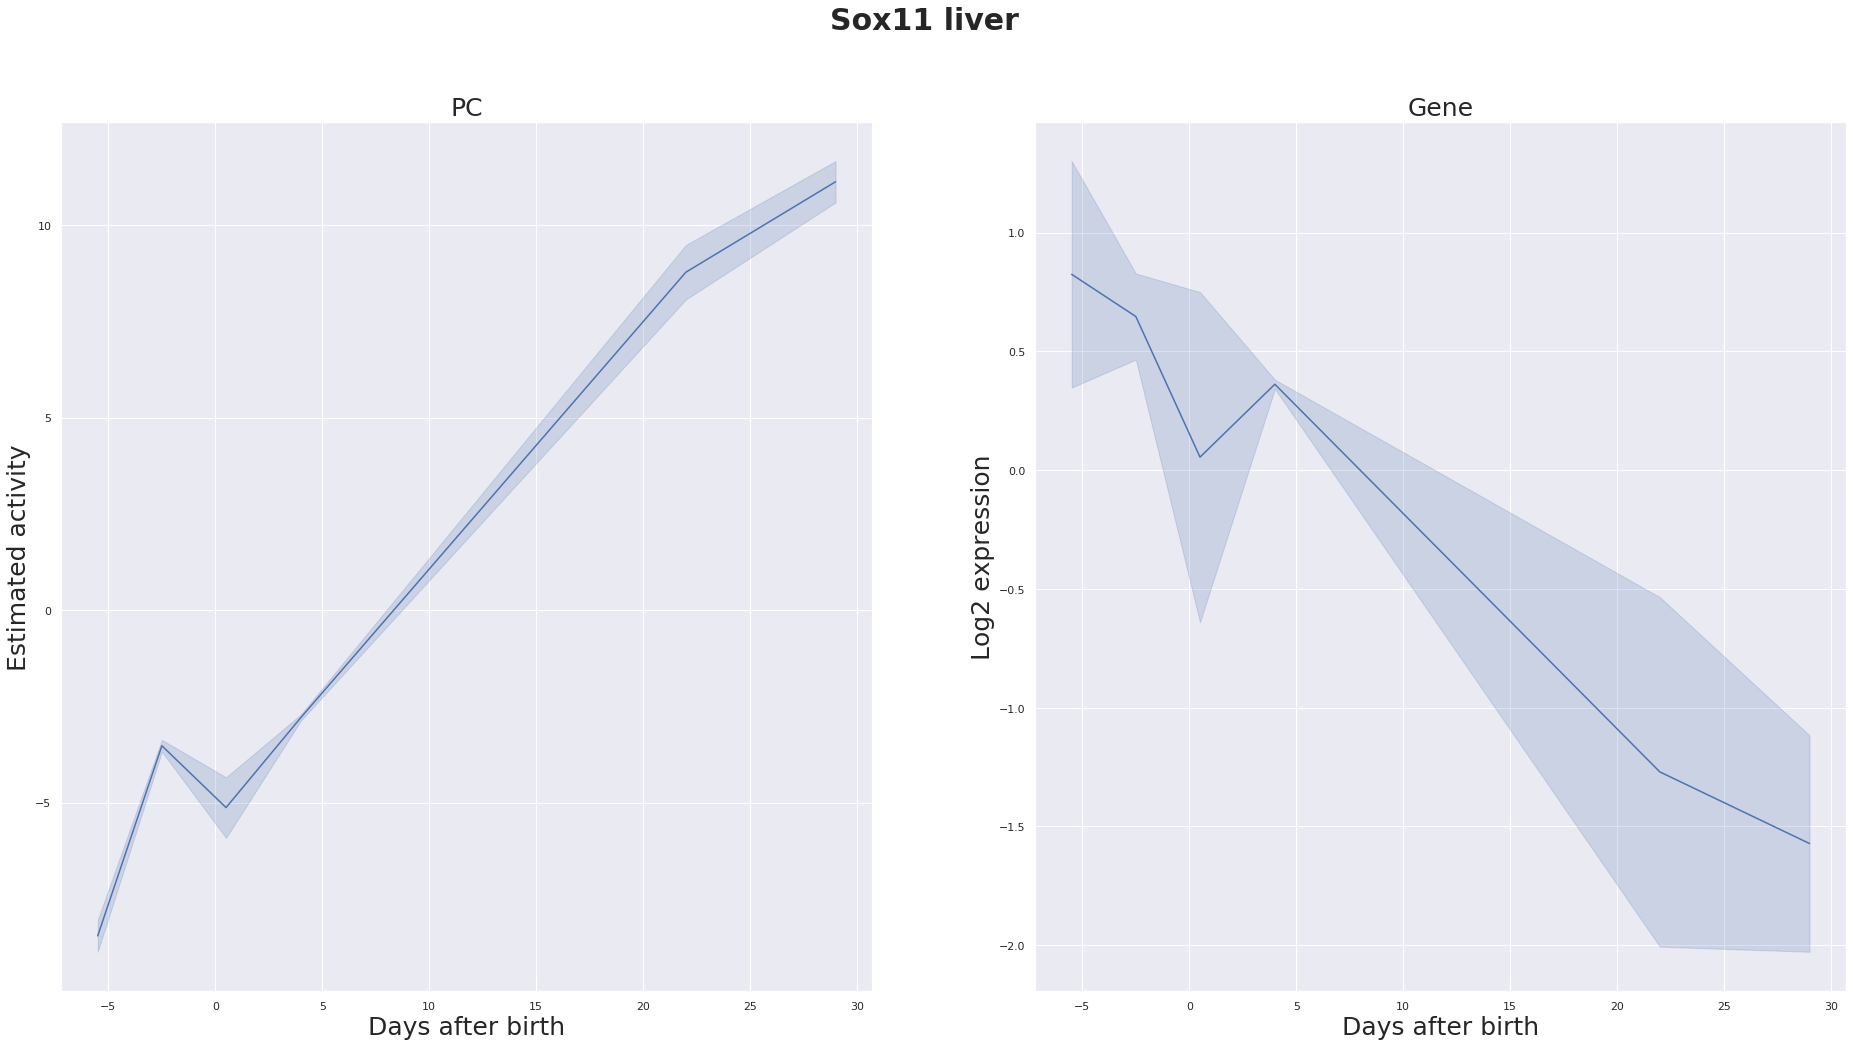
\includegraphics[width=11cm, height=5.5cm]{Figures&amp;Cover/Activity_Sox11_liver_NonePCremoved_filtering_False.png}
    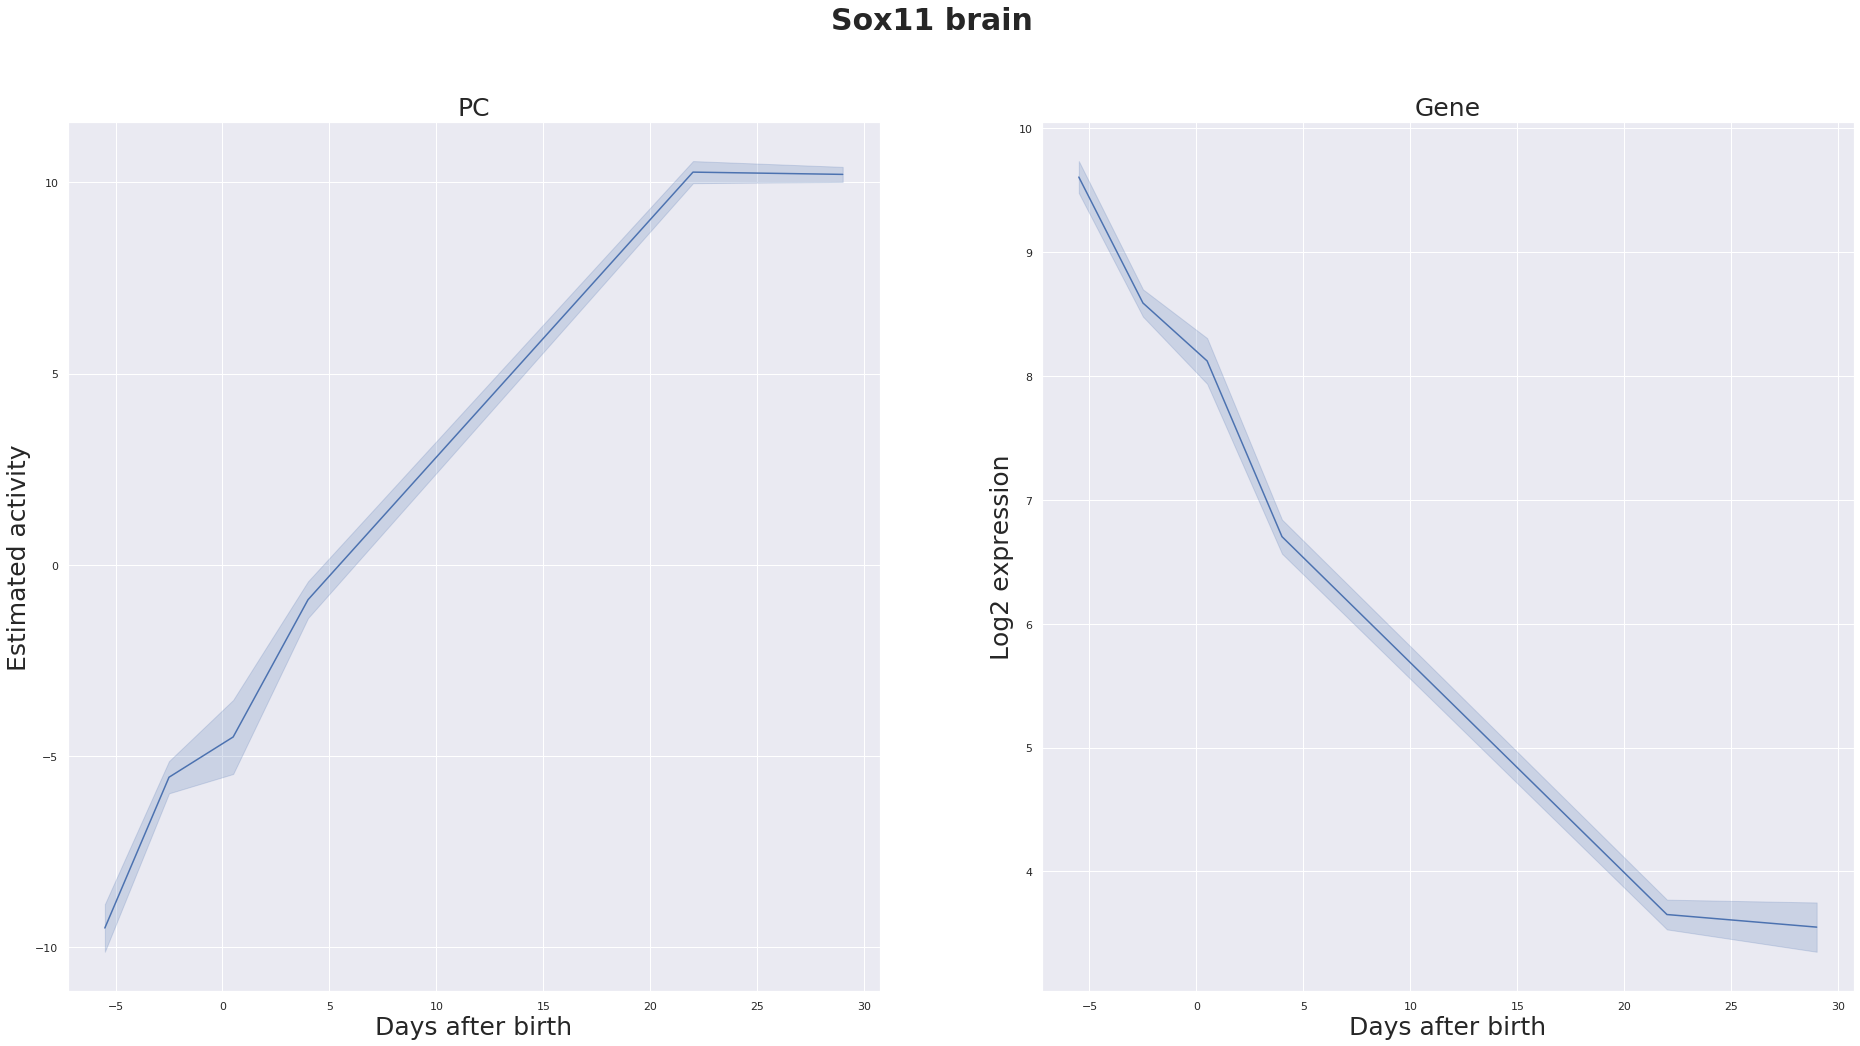
\includegraphics[width=11cm, height=5.5cm]{Figures&amp;Cover/Activity_Sox11_brain_NonePCremoved_filtering_False.png}
    \caption{\textbf{Sox11's estimated activity as a functions of mices' age.} Sox11's activity was estimated by the first \ac{PC} of the mRNA expression data of the genes it is likely to regulate (upper and lower left) as well as directly through the transcription of the genes coding for it, as log2-transformed gene count (upper and lower right). The activity estimations and mRNA expressions are from the data from mouse liver (upper left and right) and brain (lower left and right).}
    \label{fig:est_allPCs_Sox11}
\end{figure}

All of the 17 initially tested \acp{TF} shared similar trends in their activity estimations, with only slight variations. The same was true for the mRNA expressions of most \acp{TF}, but with a few exceptions as shown by the mRNA expression of Satb2 in Figure \ref{fig:est_allPCs_Satb2}. This was concerning as it indicated that the estimator was capturing a general trend in the data, possibly cause by a confounder, rather than patterns specific for the \acp{TF}. The percentage of total variance explained by the \ac{PC} used as activity estimation for each \ac{TF} was plotted, revealing that it ranged between 40-80\% and mostly clustered around 60\% for both brain and liver, as shown in Figure \ref{fig:VarExp_allPCs}. These high values further indicated that the genes measured had highly similar patterns of mRNA expression, supporting the theory of the presence of a confounder. To further investigate the existence of the trend, the first \ac{PC} for the full data set for each organ was plotted to be compared to the activity estimations and can be seen in Figure \ref{fig:firstPC}. These plots were for both organs highly similar, and their similarities to the activity estimations again indicated that there was a general trend in the data.

\begin{figure}
    \centering
    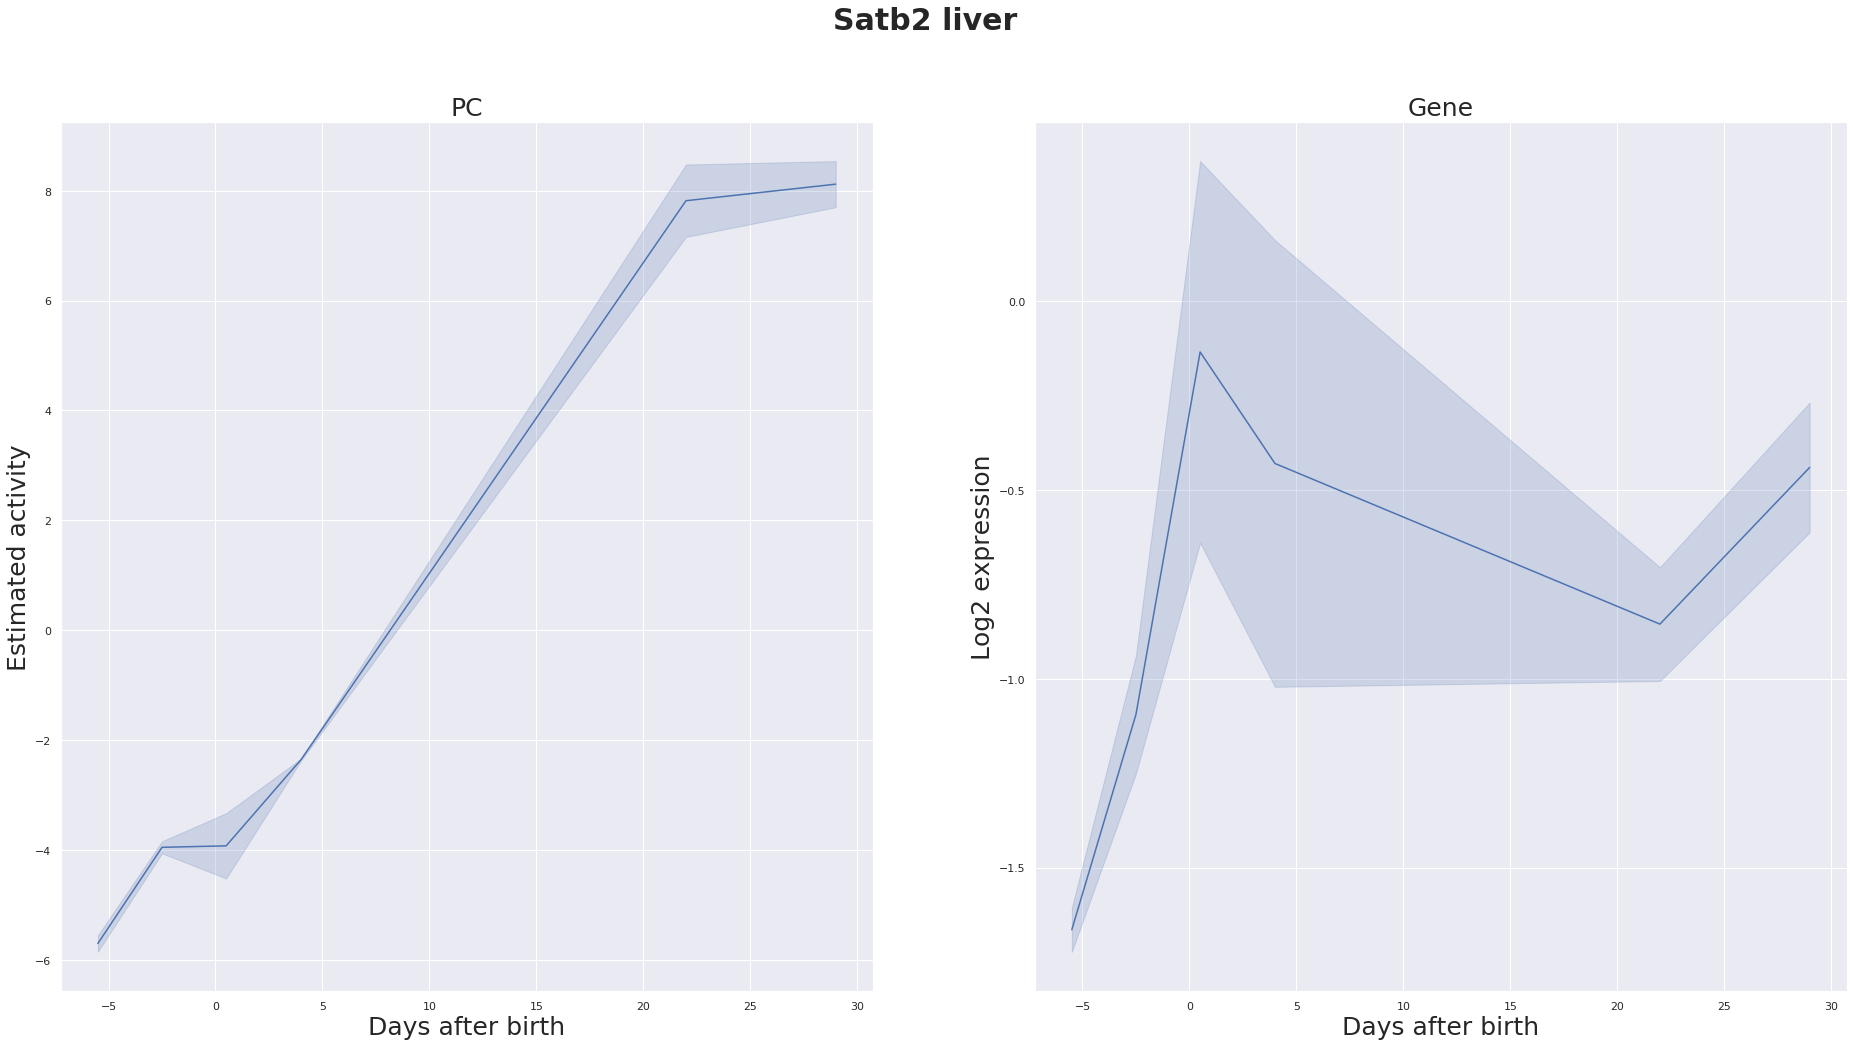
\includegraphics[width=11cm, height=5.5cm]{Figures&amp;Cover/Activity_Satb2_liver_NonePCremoved_filtering_False.png}
    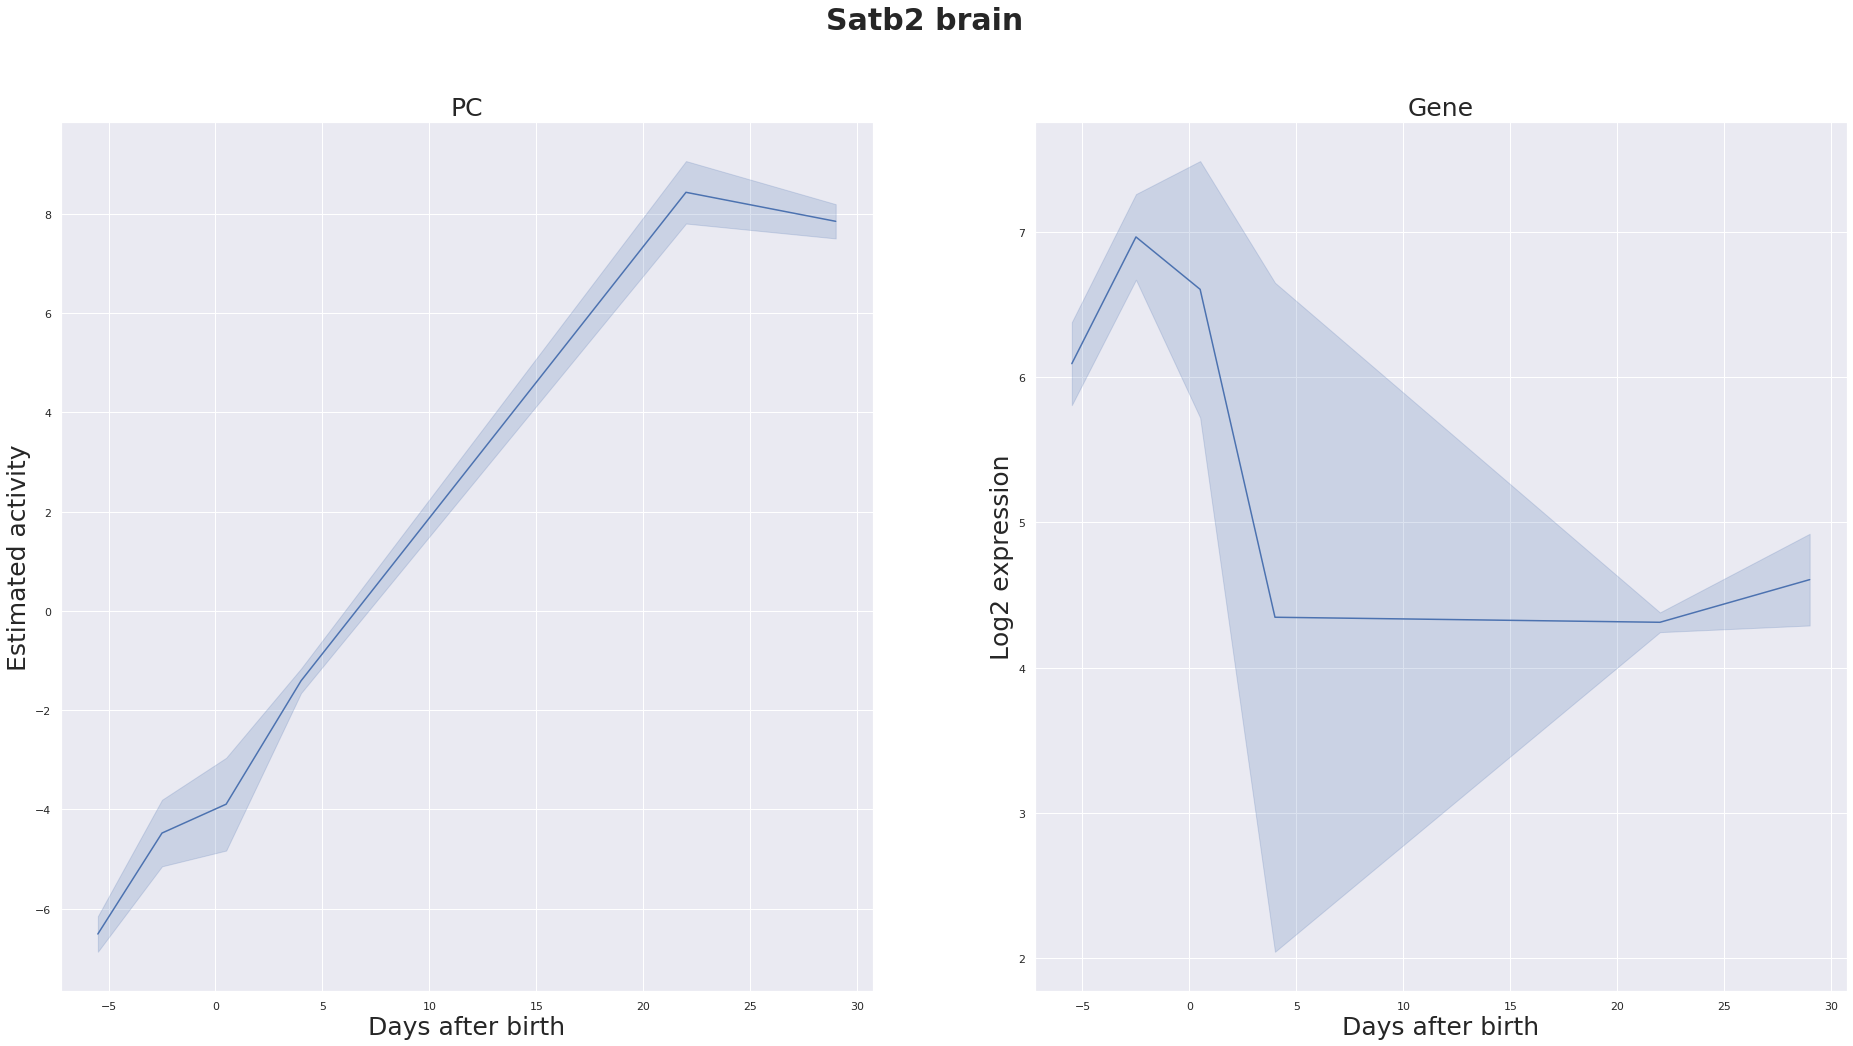
\includegraphics[width=11cm, height=5.5cm]{Figures&amp;Cover/Activity_Satb2_brain_NonePCremoved_filtering_False.png}
    \caption{\textbf{Satb2's estimated activity as a functions of mices' age.} Satb2's activity was estimated by the first \ac{PC} of the mRNA expression data of the genes it is likely to regulate (upper and lower left) as well as directly through the transcription of the genes coding for it, as log2-transformed gene count (upper and lower right). The activity estimations and mRNA expressions are from the data from mouse liver (upper left and right) and brain (lower left and right).}
    \label{fig:est_allPCs_Satb2}
\end{figure}

\begin{figure}
    \centering
    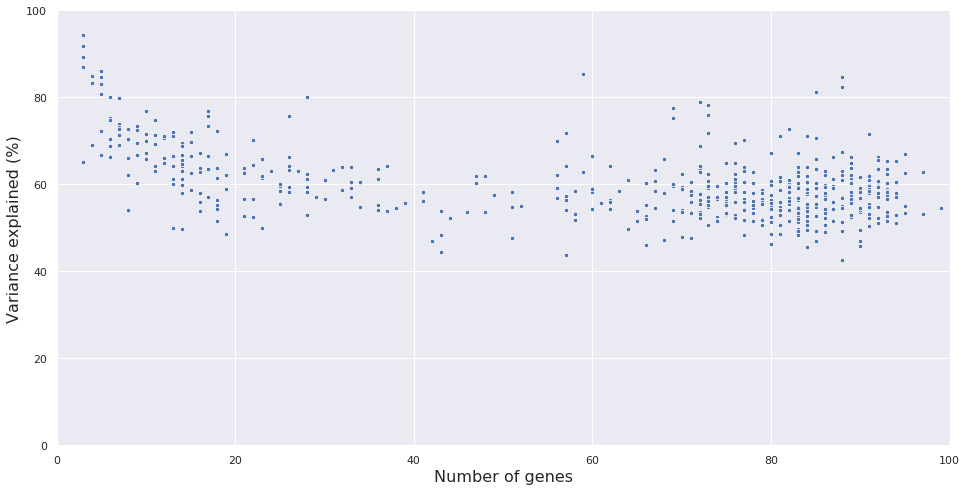
\includegraphics[width=10cm,height=5cm]{Figures&amp;Cover/VarExpl_PC1_10_300_100_liver_NonePCremoved_filtering_False.png}
    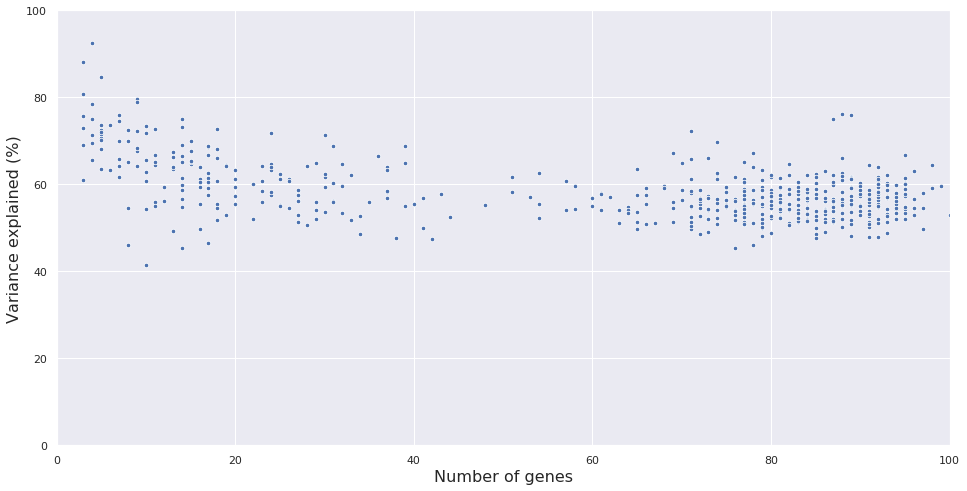
\includegraphics[width=10cm,height=5cm]{Figures&amp;Cover/VarExpl_PC1_10_300_100_brain_NonePCremoved_filtering_False.png}
    \caption{\textbf{The variance explained in the transcription data of the genes in each \ac{TF}'s gene set, as a function of the number of genes in the gene set.}  For the top plot the unmodified data from mouse liver was used and for the bottom plot the unmodified data from mouse brain. For both data sets, the first \ac{PC} is explained about 60\% of the variance, slightly more for smaller gene sets.}
    \label{fig:VarExp_allPCs}
\end{figure}

\begin{figure}
    \centering
    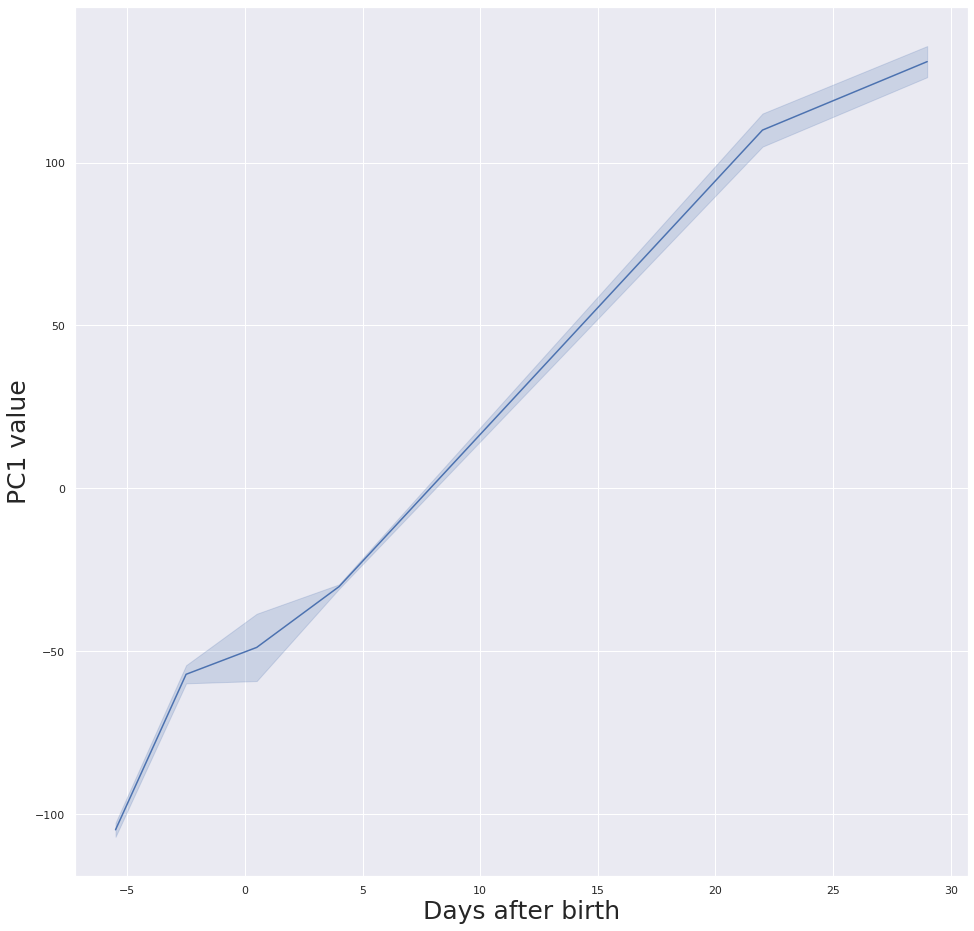
\includegraphics[width=5.5cm,height=5.5cm]{Figures&amp;Cover/Fulldata_liver_NonePCremoved_filtering_False.png}
    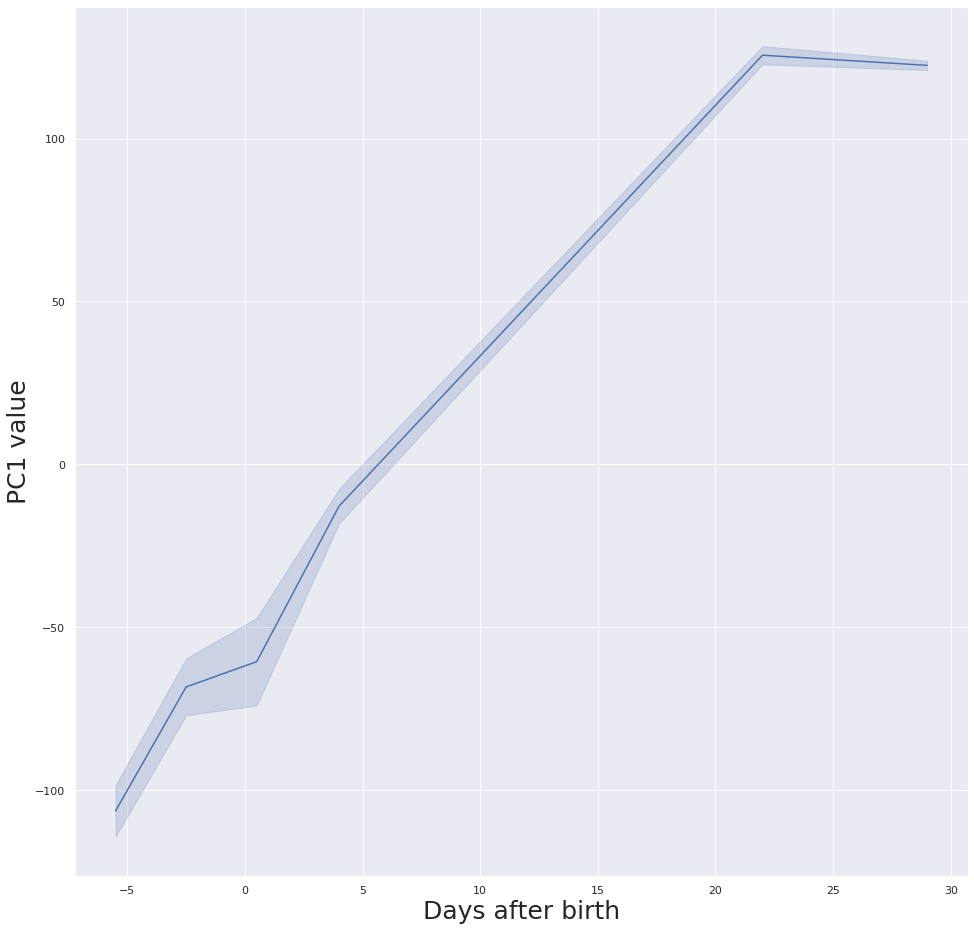
\includegraphics[width=5.5cm,height=5.5cm]{Figures&amp;Cover/Fulldata_brain_NonePCremoved_filtering_False.png}
    \caption{\textbf{The first \ac{PC} of the full sets of unmodified data from liver (left) and brain (right) as functions of age of the mice.} A very similar pattern was observed in both organs.}
    \label{fig:firstPC}
\end{figure}
\vspace{2cm}
\noindent The question then became if there was way to look past this general trend and remove the bias in the data on a global level, so variations related to specific \acp{TF} could be identified. For this purpose, \ac{PCA} was once again utilized in an attempt to remove a possible linear confounder. The data was decomposed into its \acp{PC} and then reconstructing with all but the first \ac{PC}, that encapsulated the general trend and hopefully the full effect of the confounder. When redoing the previous tests with this modified data, the similarities between the estimated activity of different \acp{TF} was overall reduced, as again exemplified with Sox11 in Figure \ref{fig:est_1PCsRemoved_Sox11}. The new estimations for all 17 \acp{TF}' activities in brain can be seen in Figure \ref{fig:BrainEstsClean1} and \ref{fig:BrainEstsClean2} in the appendix, and the estimations for their activities in liver can be seen in Figure \ref{fig:LiverEstsClean1} and \ref{fig:LiverEstsClean2} in the appendix. This was not a major concern as the correlation was expected to be far from perfect. Improvements was also seen in other cases, such as with the estimation for Satb2 as seen in Figure \ref{fig:est_1PCRemoved_Satb2}, that after the modification of the data had a similar shape to that of its gene's mRNA expression. The primary concern was however that, though less obvious, the estimations for the different \acp{TF} still appeared to follow a general trend that was also present in the mRNA expression curves. 

\begin{figure}
    \centering
    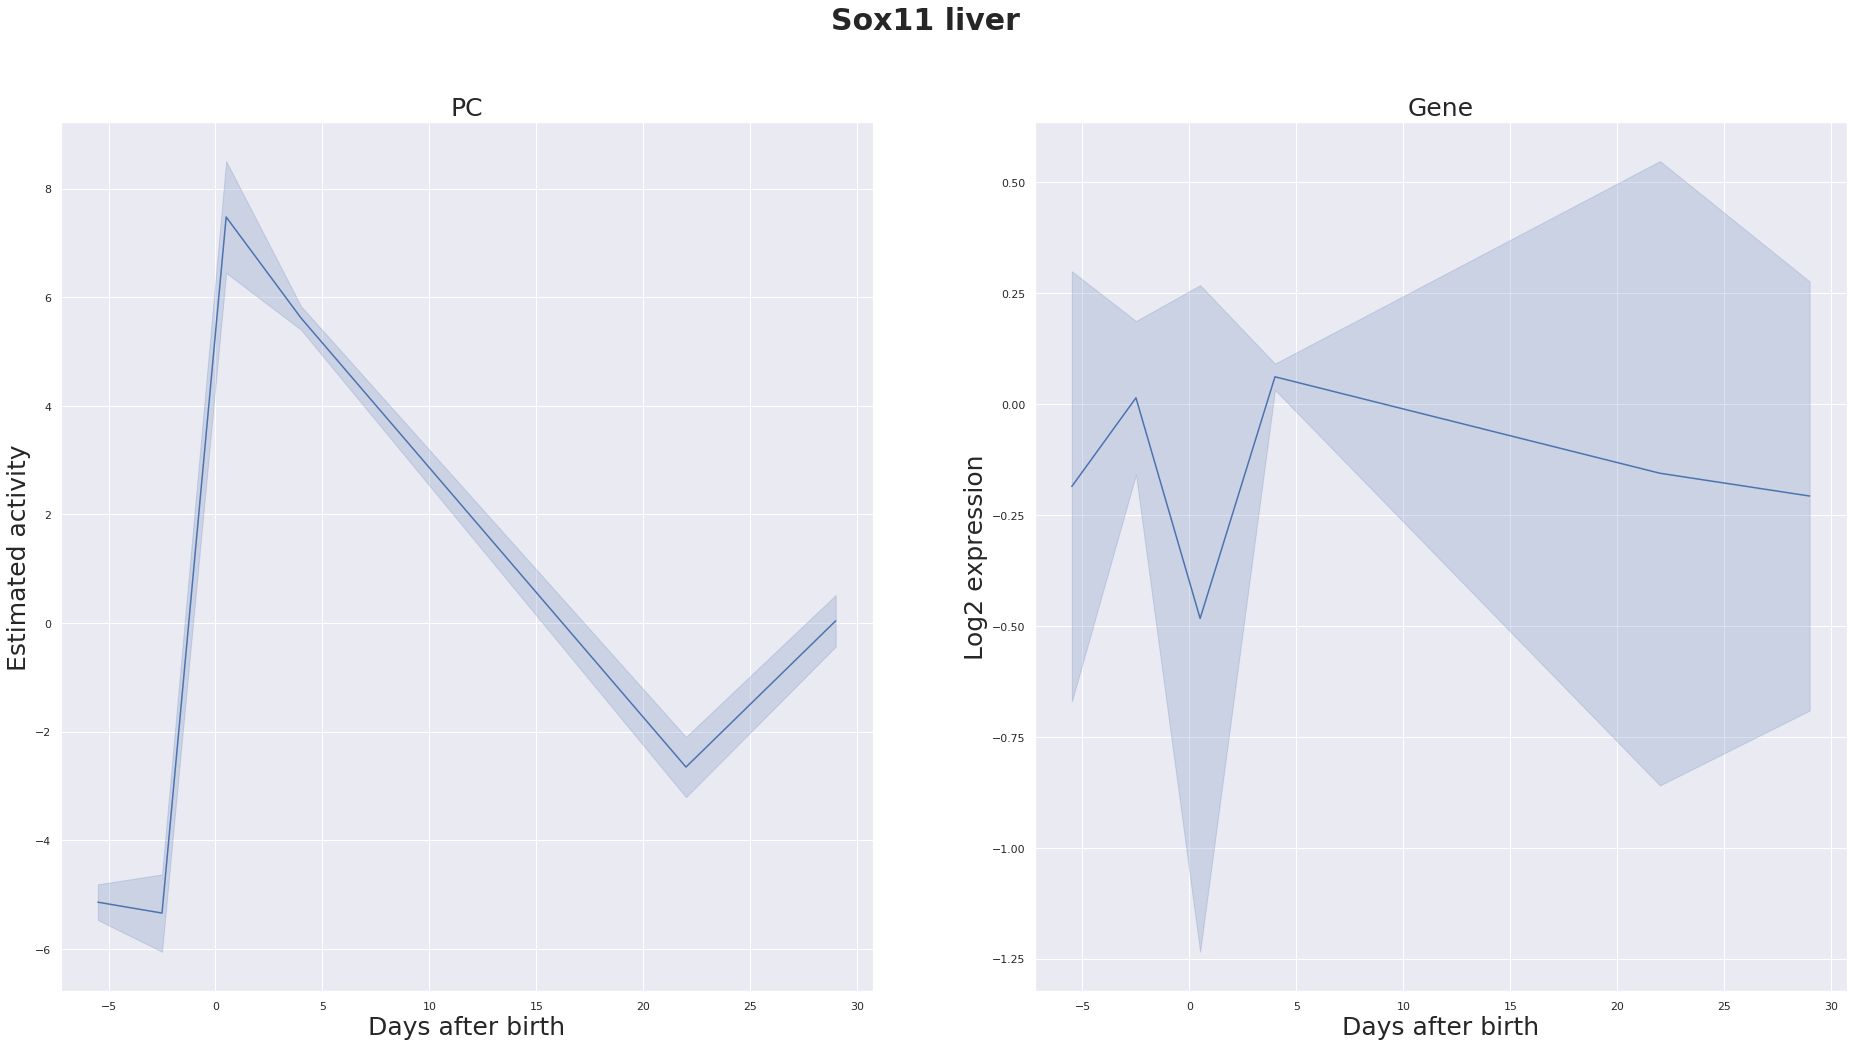
\includegraphics[width=11cm, height=5.5cm]{Figures&amp;Cover/Activity_Sox11_liver_1PCremoved_filtering_False.png}
    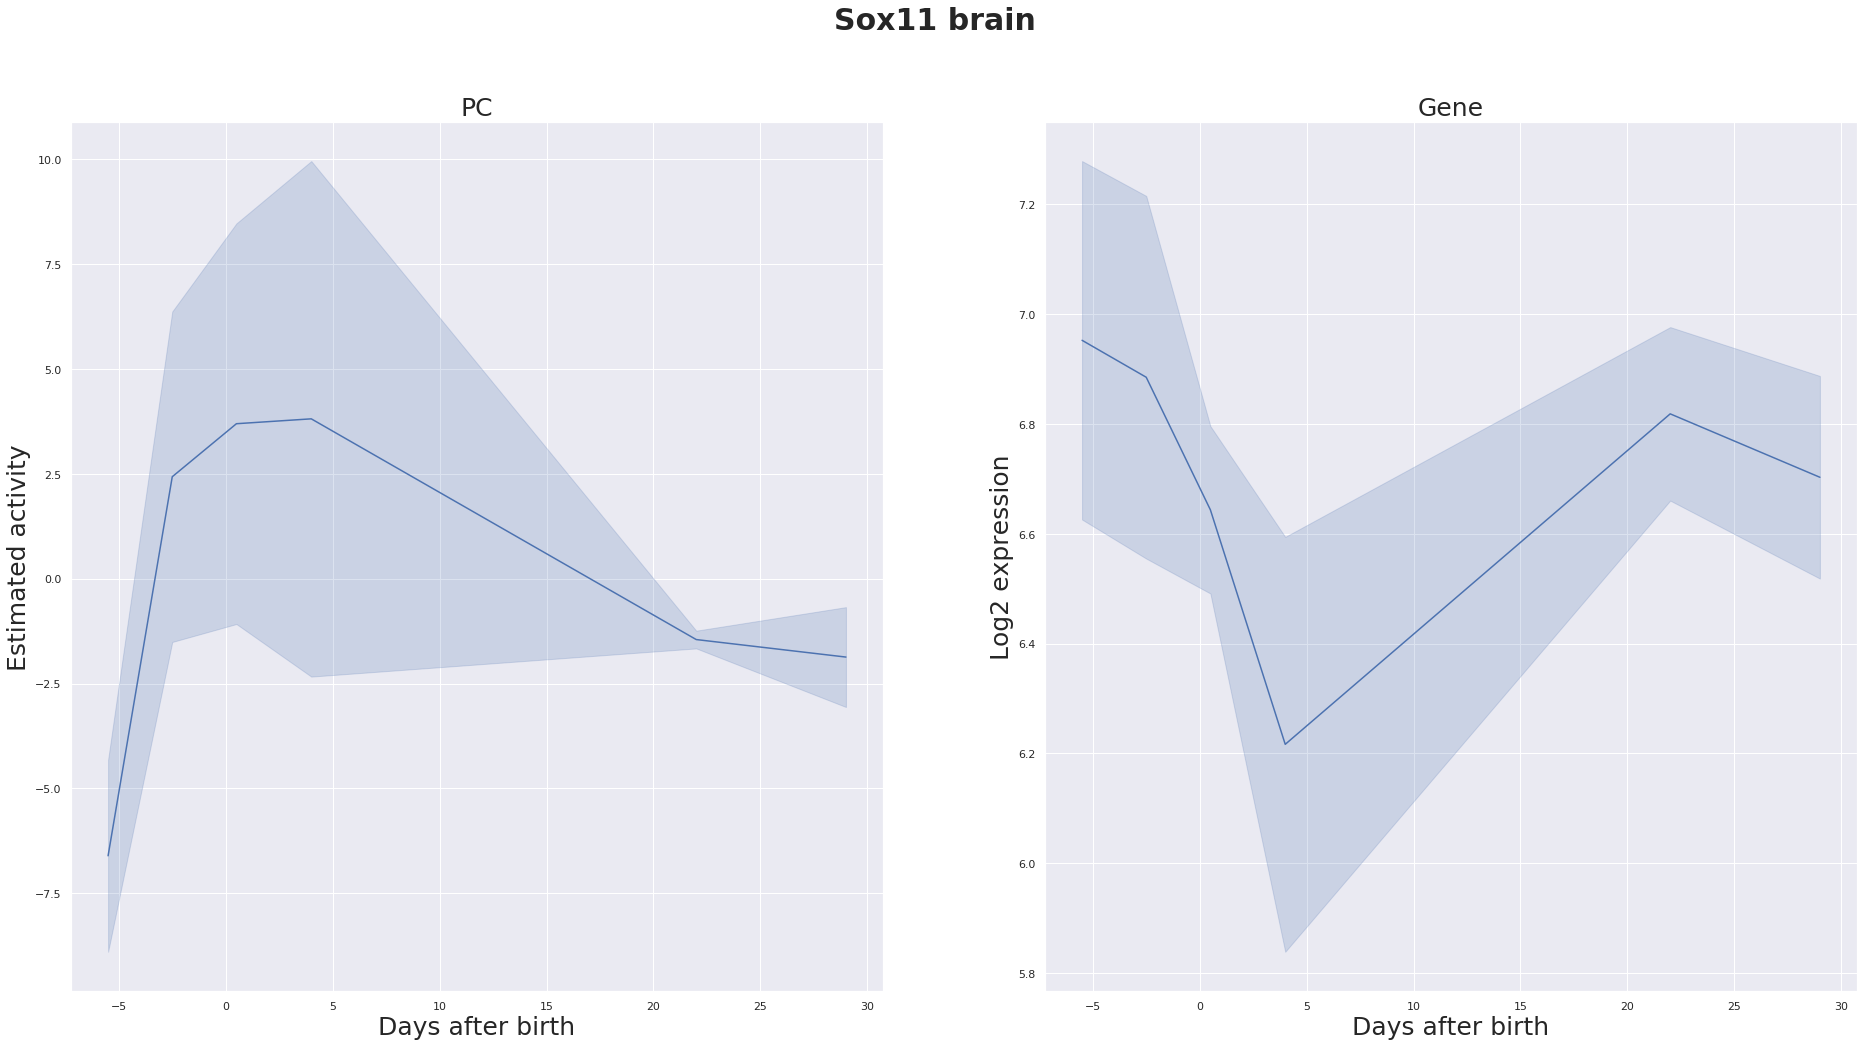
\includegraphics[width=11cm, height=5.5cm]{Figures&amp;Cover/Activity_Sox11_brain_1PCremoved_filtering_False.png}
    \caption{\textbf{Sox11's estimated activity as a functions of mices' age.} Sox11's activity was estimated by the first \ac{PC} of the mRNA expression data of the genes it is likely to regulate (upper and lower left) as well as directly through the transcription of the genes coding for it, as log2-transformed gene count (upper and lower right). The activity estimations and mRNA expressions are from the data from mouse liver (upper left and right) and brain (lower left and right) where the first \ac{PC} of the data had been removed.}
    \label{fig:est_1PCsRemoved_Sox11}
\end{figure}

\begin{figure}
    \centering
    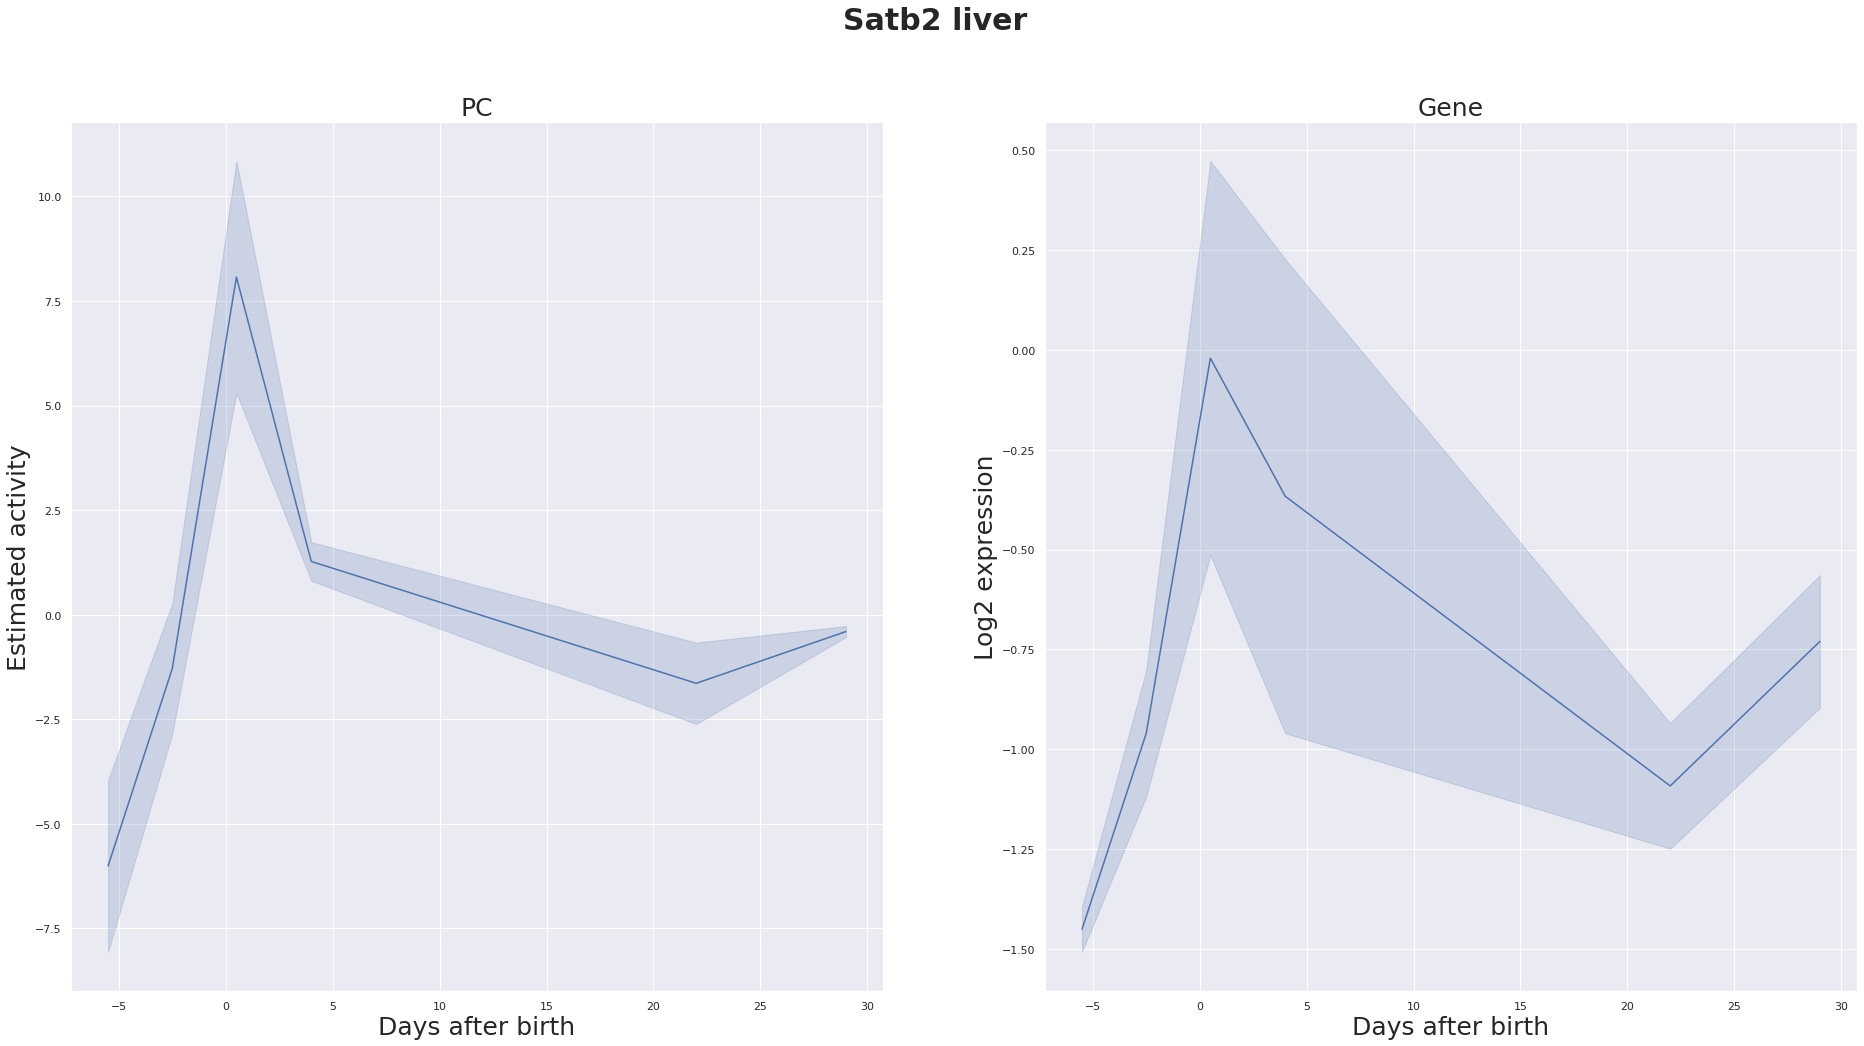
\includegraphics[width=11cm, height=5.5cm]{Figures&amp;Cover/Activity_Satb2_liver_1PCremoved_filtering_False.png}
    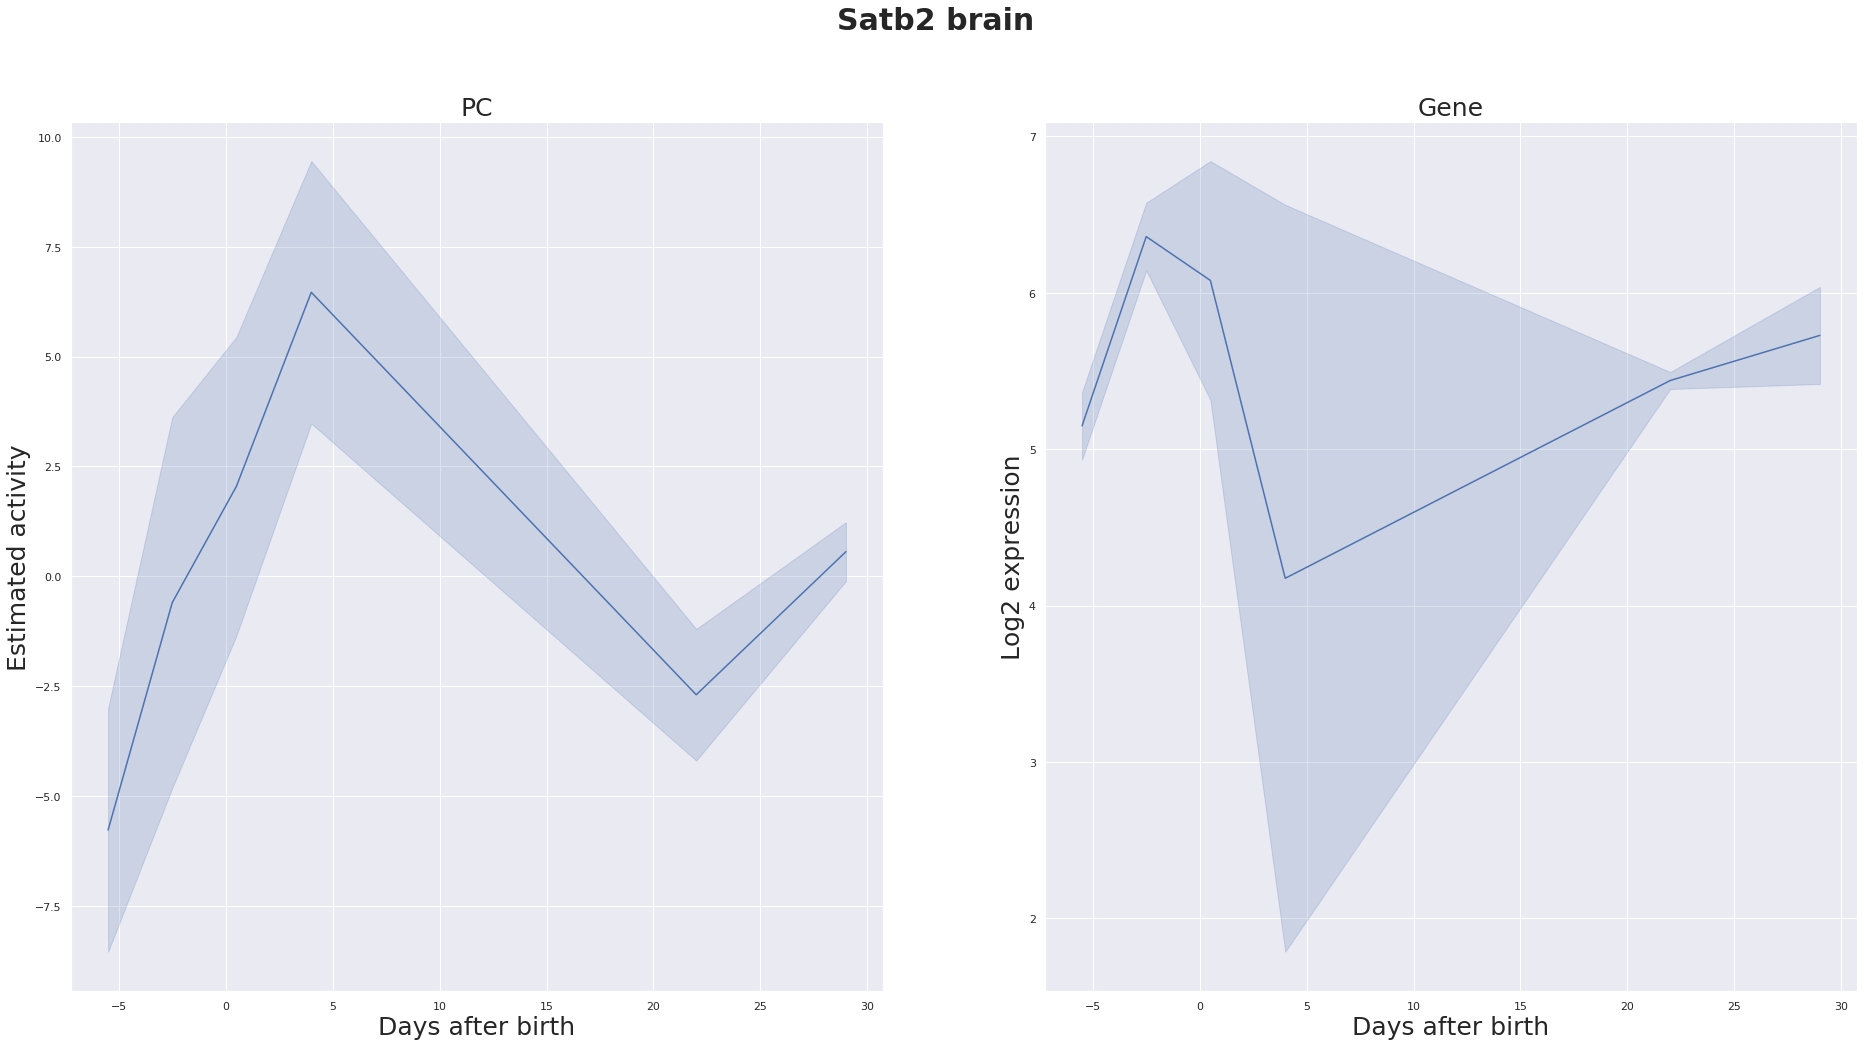
\includegraphics[width=11cm, height=5.5cm]{Figures&amp;Cover/Activity_Satb2_brain_1PCremoved_filtering_False.png}
    \caption{\textbf{Satb2's estimated activity as a functions of mices' age.} Satb2's activity was estimated by the first \ac{PC} of the mRNA expression data of the genes it is likely to regulate (upper and lower left) as well as directly through the transcription of the genes coding for it, as log2-transformed gene count (upper and lower right). The activity estimations and mRNA expressions are from the data from mouse liver (upper left and right) and brain (lower left and right) where the first \ac{PC} of the data had been removed.}
    \label{fig:est_1PCRemoved_Satb2}
\end{figure}

When the percentage of total variance explained by the \ac{PC} used as activity estimation for each \ac{TF} was plotted for the modified data it was reveled that it clustered around 35\%, but with slightly higher values for smaller gene sets, as can be seen in Figure \ref{fig:VarExp_1PCsRemoved}. This was an overall decrease of about 25 percentage points and showed that the attempt to remove the general trend had had an effect on reducing the similarities between the patterns of mRNA expression of different genes. Comparing the variance explained before and after the modification of the data gave an approximate size estimate of the linear part of the confounding effects that were removed. The results from plotting the first \ac{PC} of the complete modified data set, which is equivalent to the second \ac{PC} of the unmodified data set, can be seen in Figure \ref{fig:firstPCremoved}. The curves for the different organs were again highly similar, and when compared to the activity estimations a common, though this time much less clear, pattern could still be observed.

\begin{figure}
    \centering
    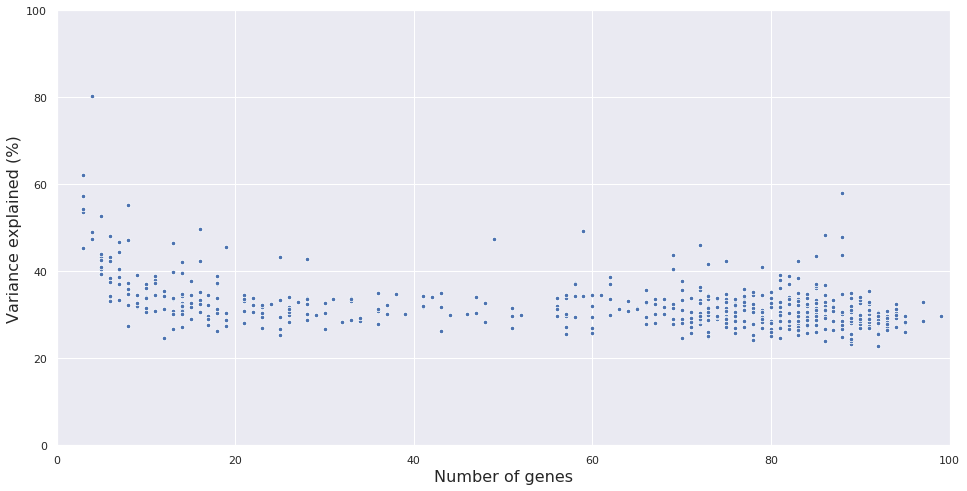
\includegraphics[width=10cm,height=5cm]{Figures&amp;Cover/VarExpl_PC1_10_300_100_liver_1PCremoved_filtering_False.png}
    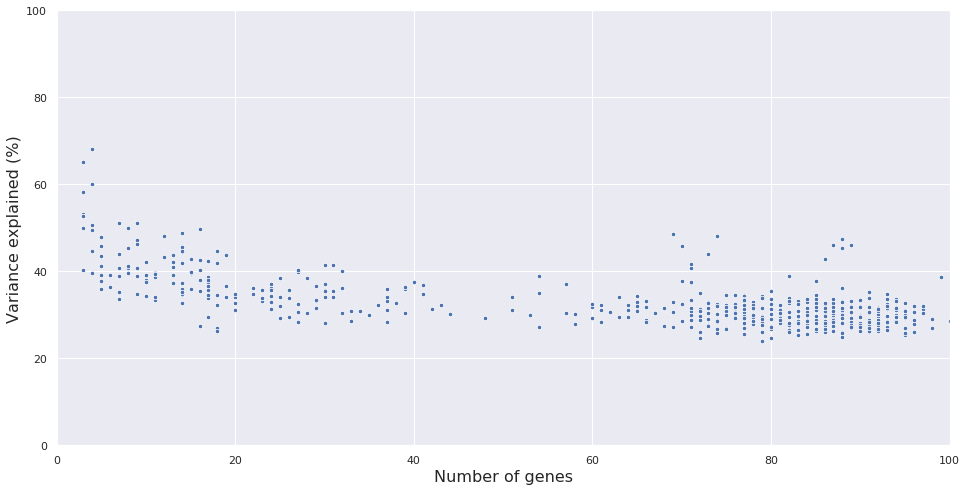
\includegraphics[width=10cm,height=5cm]{Figures&amp;Cover/VarExpl_PC1_10_300_100_brain_1PCremoved_filtering_False.png}
    \caption{\textbf{The variance explained in the transcription data of the genes in each \ac{TF}'s gene set, as a function of the number of genes in the gene set, after the data had been modified.} For the top plot the modified data from mouse liver was used and for the bottom plot the modified data from mouse brain. For both data sets, the first \ac{PC} explained about 35\% of the variance, slightly more for smaller gene sets. Comparing this to the variance explained in the gene sets with unmodified data (Figure \ref{fig:VarExp_allPCs}), where about 60\% of the variance was explained, gives an approximate size estimate of the linear part of the confounding effects that were removed.}
    \label{fig:VarExp_1PCsRemoved}
\end{figure}

\begin{figure}
    \centering
    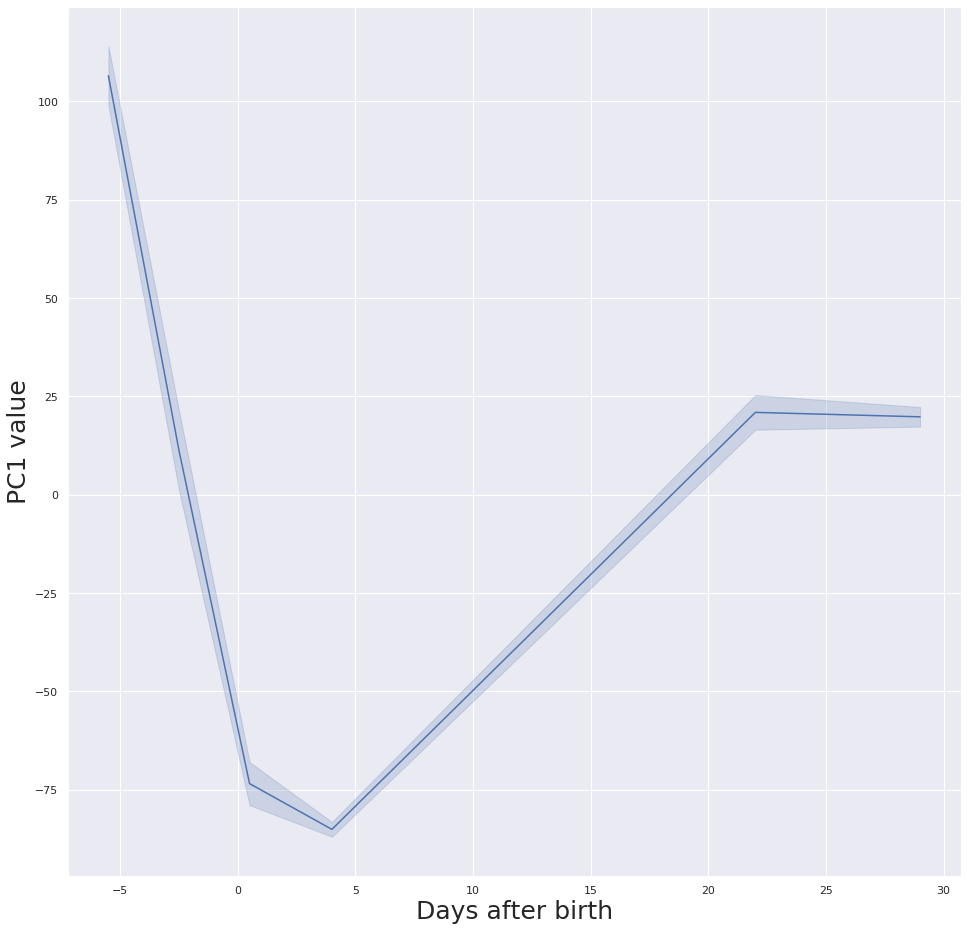
\includegraphics[width=5.5cm,height=5.5cm]{Figures&amp;Cover/Fulldata_liver_1PCremoved_filtering_False.png}
    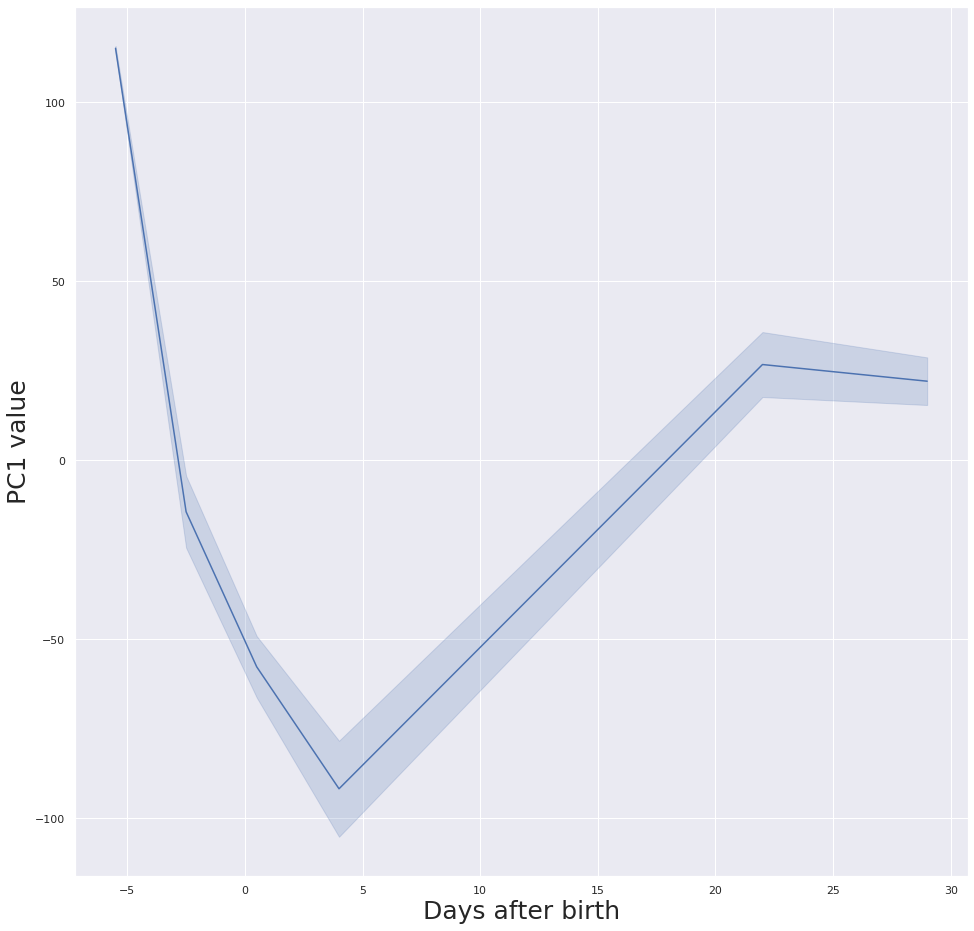
\includegraphics[width=5.5cm,height=5.5cm]{Figures&amp;Cover/Fulldata_brain_1PCremoved_filtering_False.png}
    \caption{\textbf{The first \acp{PC} of the full sets of modified data from liver (left) and brain (right) as functions of age of the mice.} The data was modified by removing the first \ac{PC} prior to analysis, meaning that this is equivalent to the second principal component for the unmodified data.}
    \label{fig:firstPCremoved}
\end{figure}




\chapter{Discussion}
\vspace{-0.75cm}
\ac{PCA} is method that captures general trends in data, and the intent in this project was to isolate different trends by applying it to different extracts from a data set. This failed however, due to the strong common trend that was present in the data that caused all \ac{TF} activity estimations to be highly similar. This could be due to an inhered problem with the estimator and the assumptions it is based on, but could also be caused by problems with the data. If the trend was caused by a technical confounder the estimator could still have potential, but if the trend was indeed caused by biological factors it would mean that the assumptions were too distinct from reality. To determine the potential of the estimator further testing is therefore required.

The method applied in an effort to remove the confounder was, as the results showed, not fully successful. Removing the first \ac{PC} from the full data additionally meant that what was used for the analysis was no longer the actual measured mRNA expression, which complicated the interpretation of whatever results were obtained. It should also be considered that removing the first \ac{PC} from a data set means that a significant portion of the information the data contains is lost, and that it could potentially introduce new biases.

The estimator relies on the assumption that genes regulated by a common \ac{TF} share an identifiable unique common pattern in their mRNA expression, and that the \ac{TF} is the overall primary source of variation in their mRNA expression. This is however a gross simplification of the mechanics of \ac{TF} regulation. As described in Chapter \ref{sec:background}, many \acp{TF} act in a cooperative manner where the regulatory effect differs from the sum of its parts. Each gene regulated by a \ac{TF} has a different set of other regulators affecting its transcription, all with varying and changing levels of presence. The effect of the presences of the specific \ac{TF} could thus be either substantial, nonexistent or anything in between, depending on the gene and time point. It is thus unlikely that the investigated \ac{TF} is the primary source of variation in the mRNA expression of the genes in its set. Though, if the effects of the single \ac{TF} is not entirely obscured an idea could be to look into other \acp{PC} than the first to see if there are less obvious common pattern among the genes the \ac{TF} regulates. This however presents the issue of knowing which \ac{PC} to use for the estimation.

Another assumption of the model is that there is a linear correlation between \ac{TF} activity and mRNA expression of its gene. This does often not hold true in reality, even if all other prerequisites for its regulatory effect are fulfilled, as \acp{TF} can act closer to an on/off switch rather than increasing mRNA expression relative to concentration. Saturation effect could potentially also occur at high concentrations of a \ac{TF}, where there is no change in regulation despite increased concentration of the \ac{TF}. This assumption of a linear correlation is however inherited from the use of \ac{PCA} and must be accepted as a limitation of the estimator.

Without making major changes to the estimator, improved results could possibly be achieved by revising the gene sets used to define which genes individual \acp{TF} regulates. The sets directly taken from ChIP-Atlas are only a rough prediction of genes regulated by specific \acp{TF} based on proximity and are as a result also very large and likely to contain much noise. The method applied to compensate for this was, partly due to lack of options, equally crude and could with no certainty produce gene sets containing genes clearly regulated by the specified \ac{TF}. Though sets of genes with more assured association with each respective \ac{TF} are expected to become available in the future through the continued experimental efforts of mapping \ac{TF} regulation, it will take a long time until such data has the same coverage as ChIP-seq data has today. Another improvement that should be made is to make the gene sets for each organ individually since, as previously mentioned, \ac{TF} regulation in cases can be tissue specific.

\chapter{Future perspectives}
\vspace{-0.75cm}
From the tests performed in this project a final statement of the potential of the estimator can not be given for mainly two reasons; the expression data it was applied to and the method used for validation. 

To answer the question if the issues encountered in this project was caused by problems with the data or the estimator, further testing should be performed on other data sets. Parameters to consider for these include their complexity and the time frame of  sampling. In terms of complexity, the estimator could work better with data from simpler organisms, where there are less factors influencing mRNA expression. In terms of time frame, the time between sampling points was for the data used in this project multiple  days, so it could be of interest to test if the estimator can produce better results when estimating changed occurring over a shorter period. 

Comparing the estimated activity of a \ac{TF} to the mRNA expression of the gene coding for it, as done in this project, makes it impossible to claim that the estimator is any more accurate than simply looking at the mRNA expression. For further testing, other validation methods must therefore be employed. Ideal would be to compare estimated values to experimental values, which could be done after conducting a targeted experiment where, for a set period, the mRNA expression of all regulated genes is measured while in parallel performing an assay for measuring the activity of a selection of \ac{TF}. This way, estimations could be made with the mRNA expression data and the experimental activity values could be used as a ground truth for comparison. As such an experiment would be costly however, an alternative method could be to compare the results of the estimator to that of other available estimators, such as ISMARA. But without a reliable ground truth, it is difficult to make claims about the accuracy of the estimator.

 For further development on the estimator, the likely most important thing to look into is ways to take the cooperative binding of \acp{TF} into account. That this is necessary could not be determined in this project, but since it is key to their regulatory effects it can be expected to be significant for producing accurate estimations of \ac{TF} activity. 
 
\chapter{Acknowledgements}
\vspace{-0.75cm}
I would first of like to thank my supervisor, Lukas Käll, for having offered me this project, for all the help and advice he has given throughout, and for believing in me till the end. A huge thank you is also owed to my co-supervisor Gustavo Jeuken for all his help and kindness. 

I am also grateful for the expert input on transcription factors received from by Marcel Tarbier, the gene expression data provided by Claudia Kutter's lab at SciLifeLab, as well as for all the friendly advice and input I have received from Partik Bjärterot, who performed his master project supervised by Lukas Käll during the same time period. Thank you all.


% Print the bibliography (and make it appear in the table of contents)

\printbibliography[heading=bibintoc]

\appendix

\chapter{Supplementary figures}
\label{sec:plotsetc}
\vspace{-0.75cm}

\begin{figure}
    \centering
    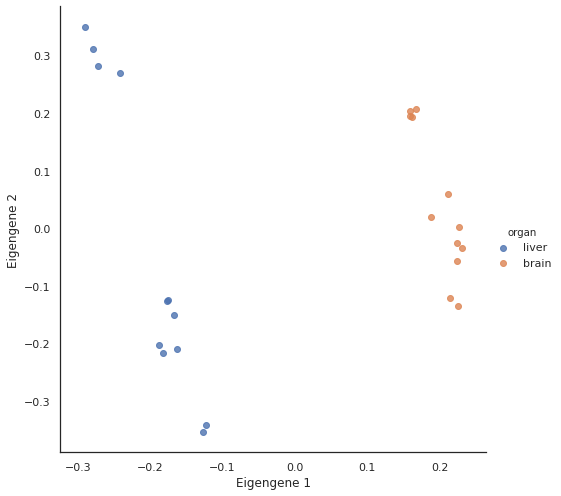
\includegraphics[width=7cm, height=7cm]{Figures&amp;Cover/SampleBehaviourorgan.png}
    \caption{\textbf{Sample behaviour of the preprocessed mRNA expression data.} The mRNA expression data from \textit{M. musculus} liver and brain, that had been \ac{RPM} normalized and log2-transformed, was decomposed using singular value decomposition and the first and second eigengenes were plotted against each other. The samples were coloured by the organ they were sampled from, blue for liver samples and orange for brain samples.}
    \label{fig:SampleBehaviour}
\end{figure}

\begin{figure}
    \centering
    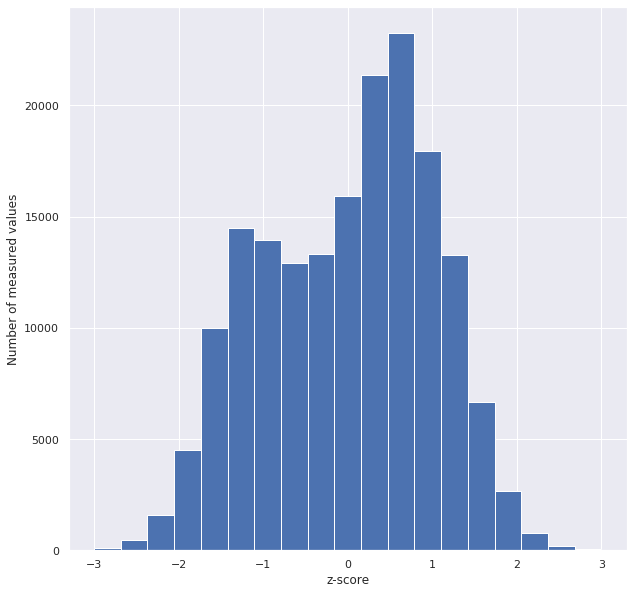
\includegraphics[width=6cm, height=6cm]{Figures&amp;Cover/logdatadistLiver.png}
    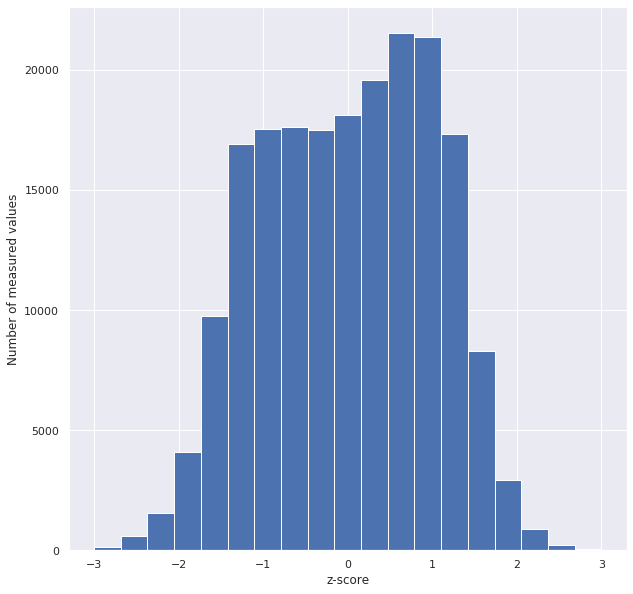
\includegraphics[width=6cm, height=6cm]{Figures&amp;Cover/logdatadistBrain.png}
    \caption{\textbf{Distribution of z-scores for the preprocessed mRNA expression data from \textit{M. musculus} liver (left) and brain (right)}. The z-scores for the mRNA expression values from liver and brain that had been \ac{RPM} normalized and log2-transformed was for each gene calculated and the results were gathered and plotted as a histogram to confirm that they were normally distributed.}
    \label{fig:logdatadist}
\end{figure}

\begin{figure}
    \centering
    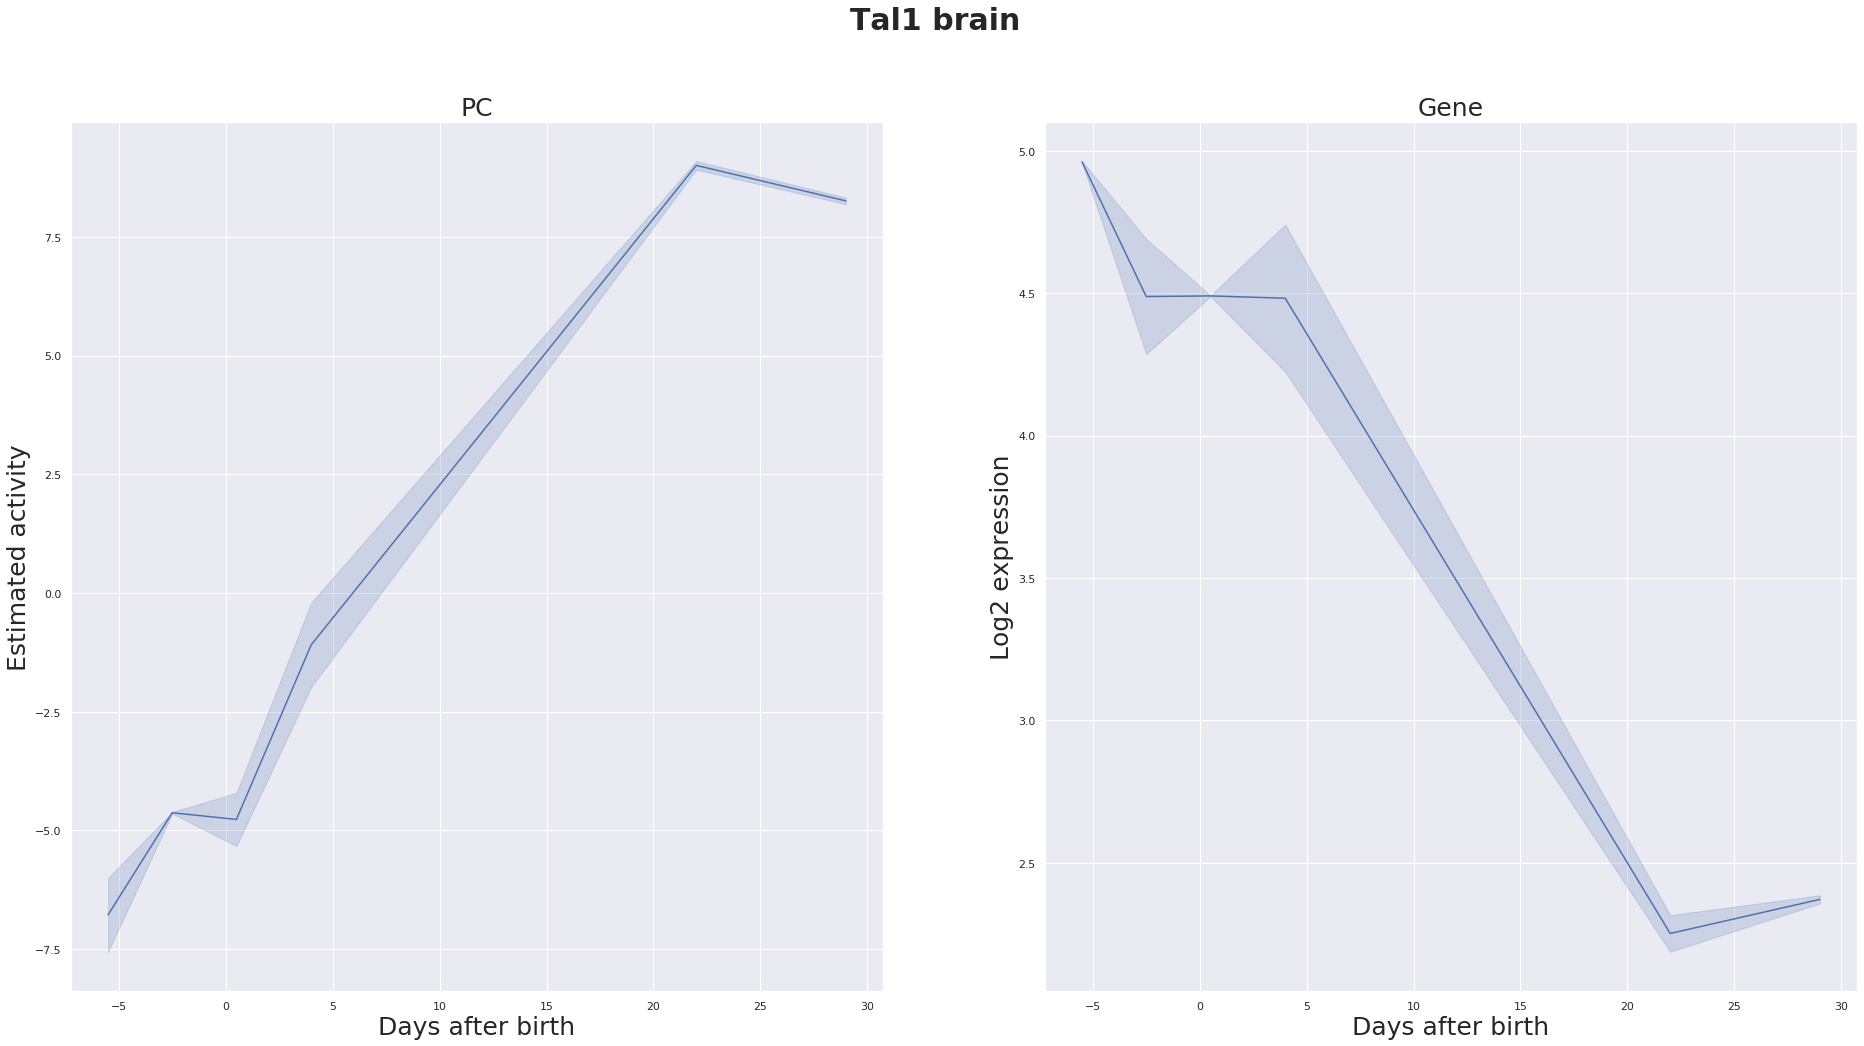
\includegraphics[width=6cm,height=3cm]{Figures&amp;Cover/Activity_Tal1_brain_NonePCremoved_filtering_False.png}
    \hspace{0.25cm}
    \vspace{0.25cm}
    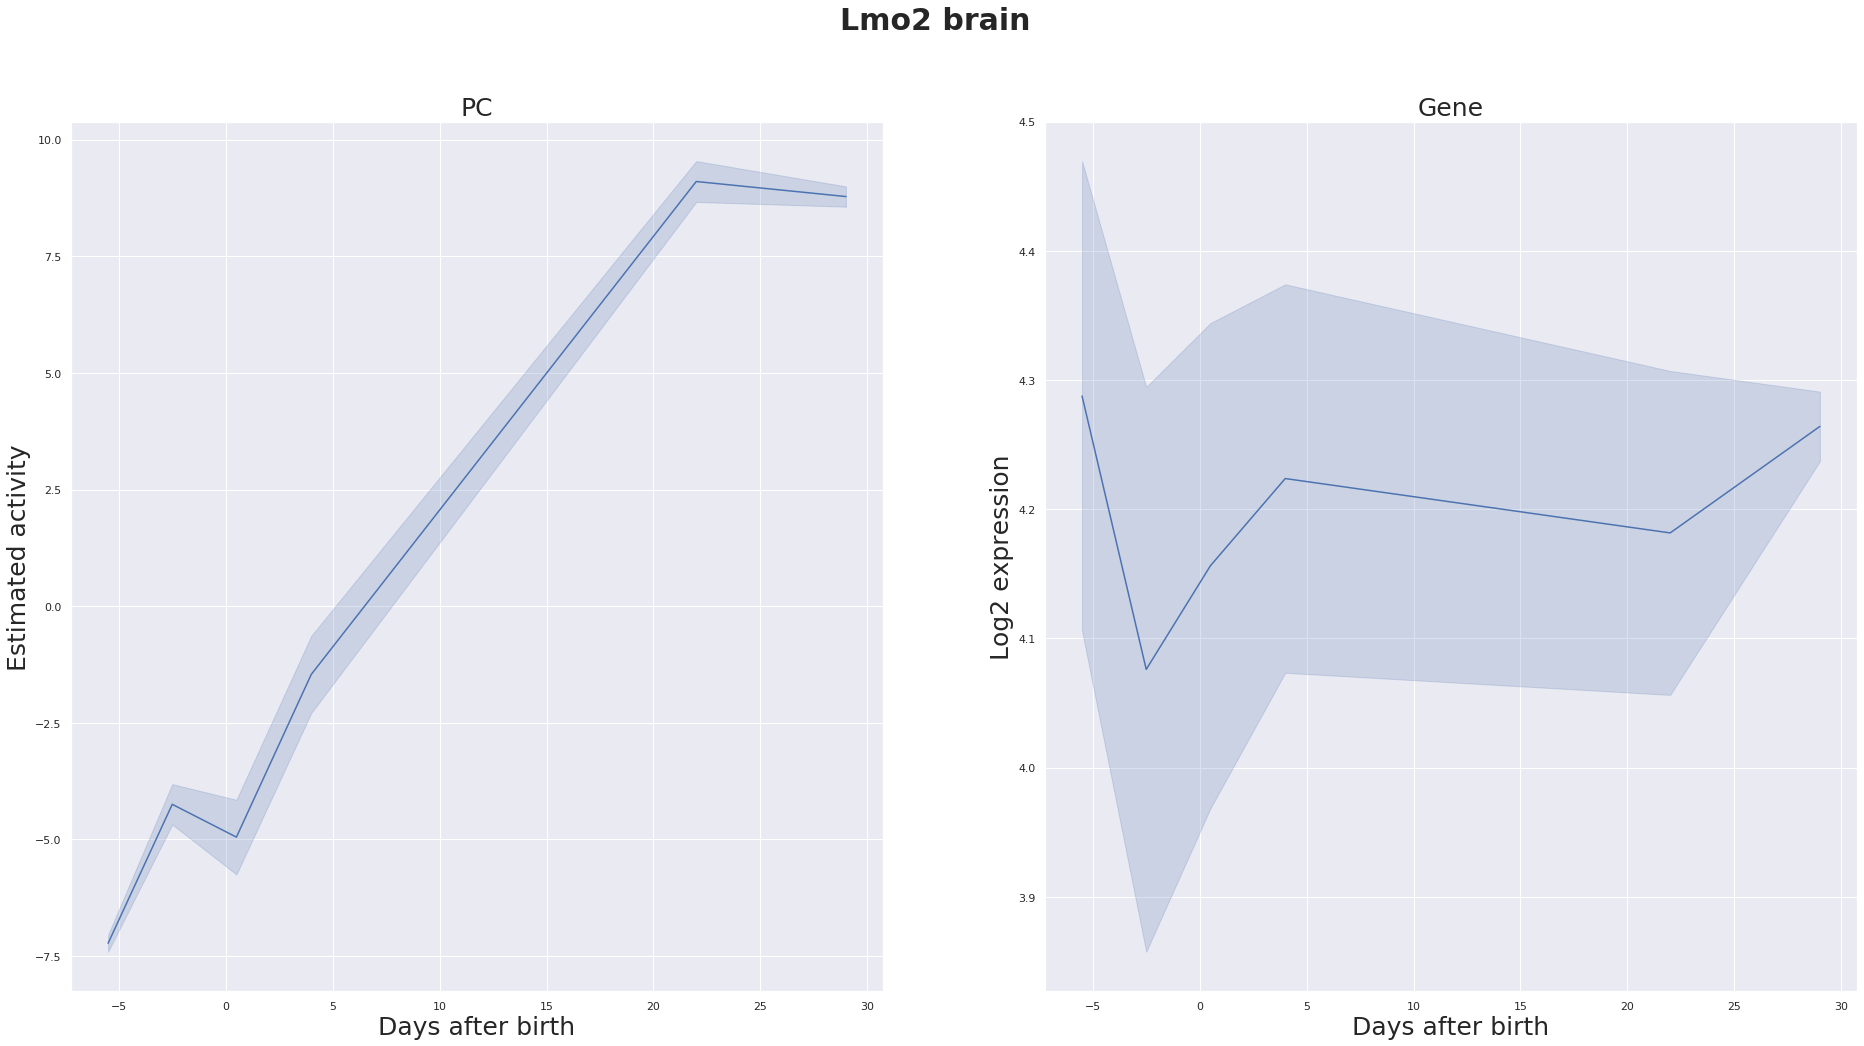
\includegraphics[width=6cm,height=3cm]{Figures&amp;Cover/Activity_Lmo2_brain_NonePCremoved_filtering_False.png}
    \vspace{0.25cm}
    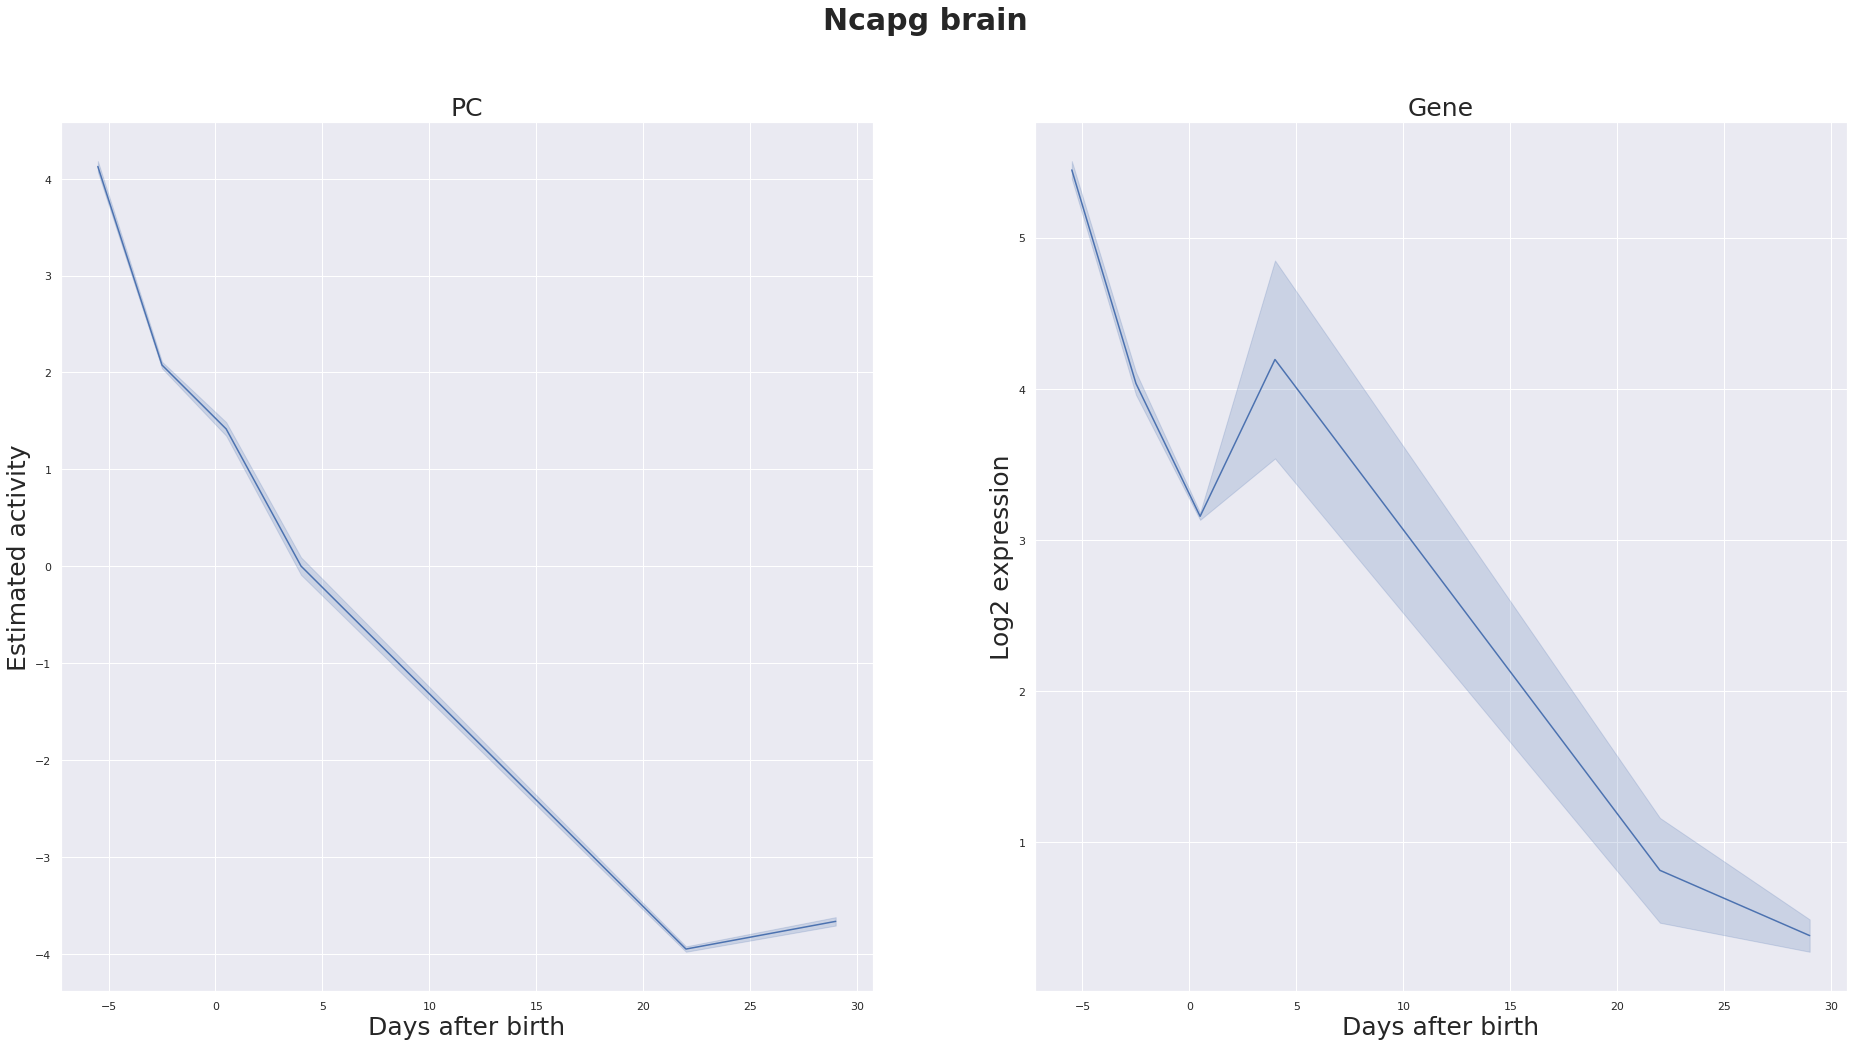
\includegraphics[width=6cm,height=3cm]{Figures&amp;Cover/Activity_Ncapg_brain_NonePCremoved_filtering_False.png}
    \hspace{0.25cm}
    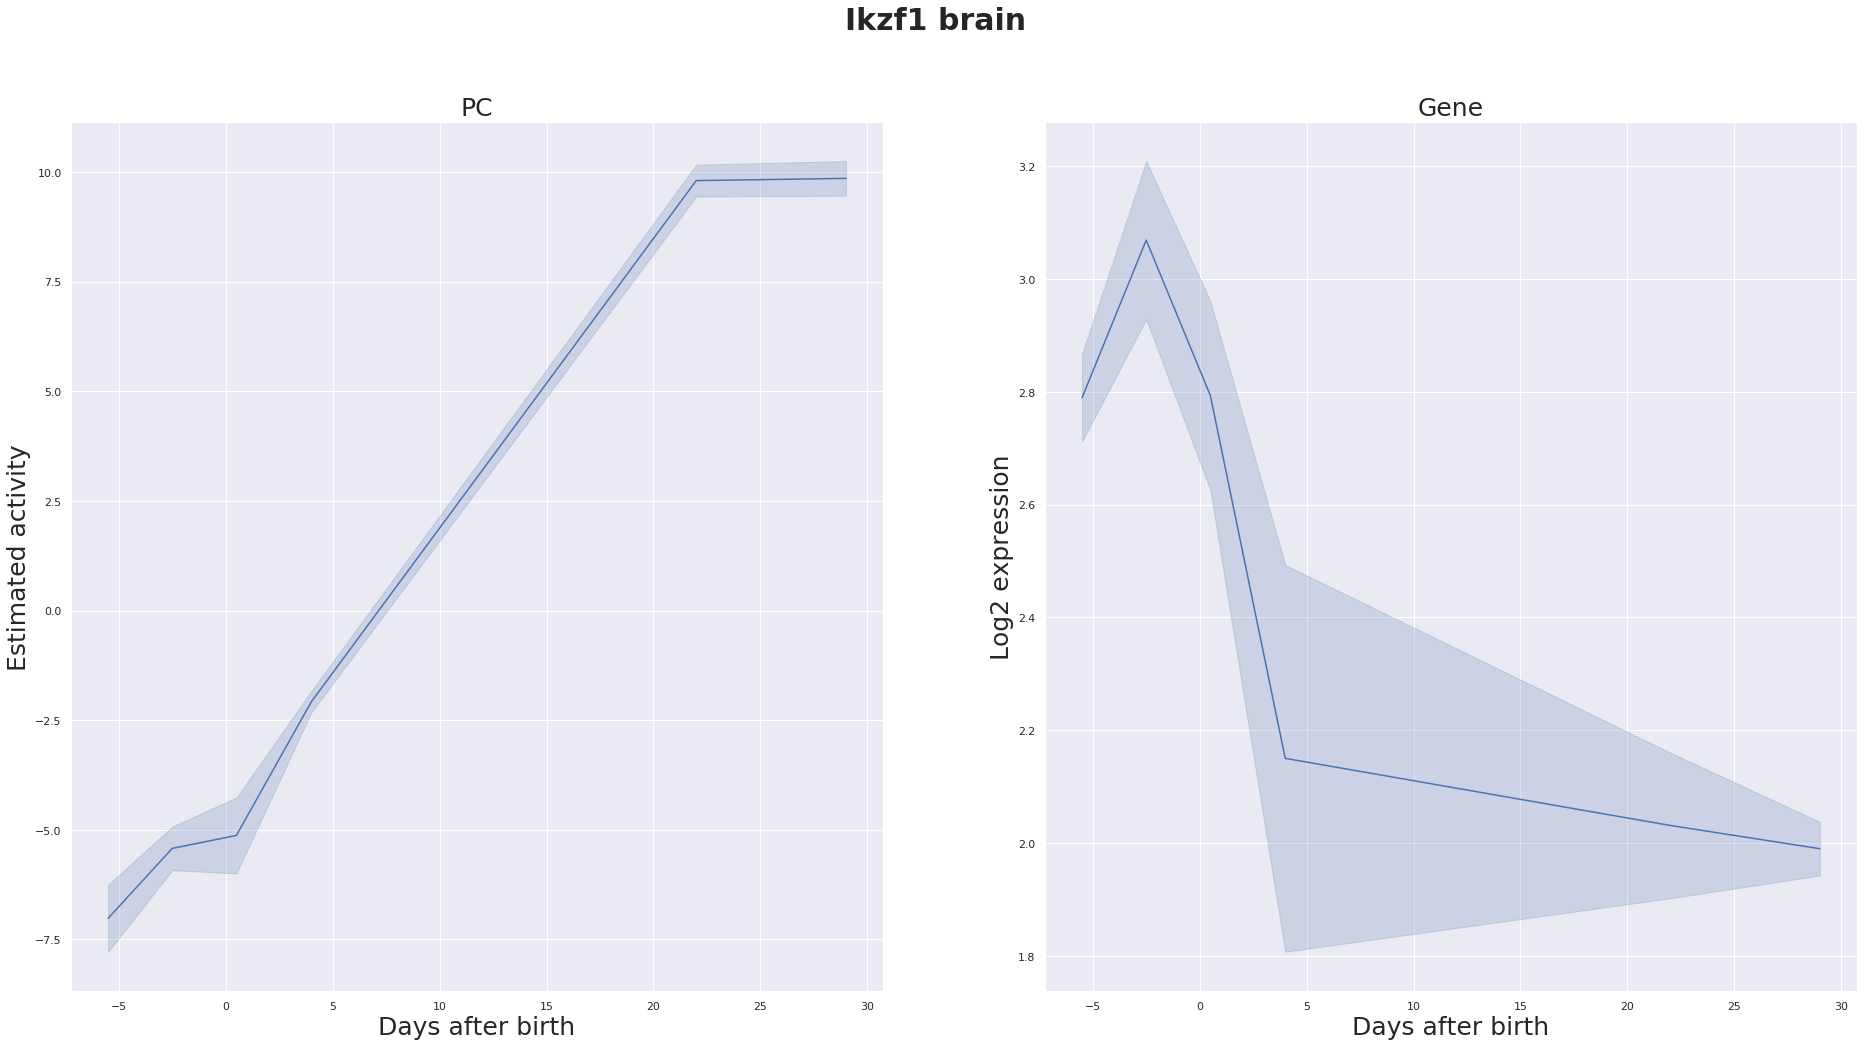
\includegraphics[width=6cm,height=3cm]{Figures&amp;Cover/Activity_Ikzf1_brain_NonePCremoved_filtering_False.png}
    \vspace{0.25cm}
    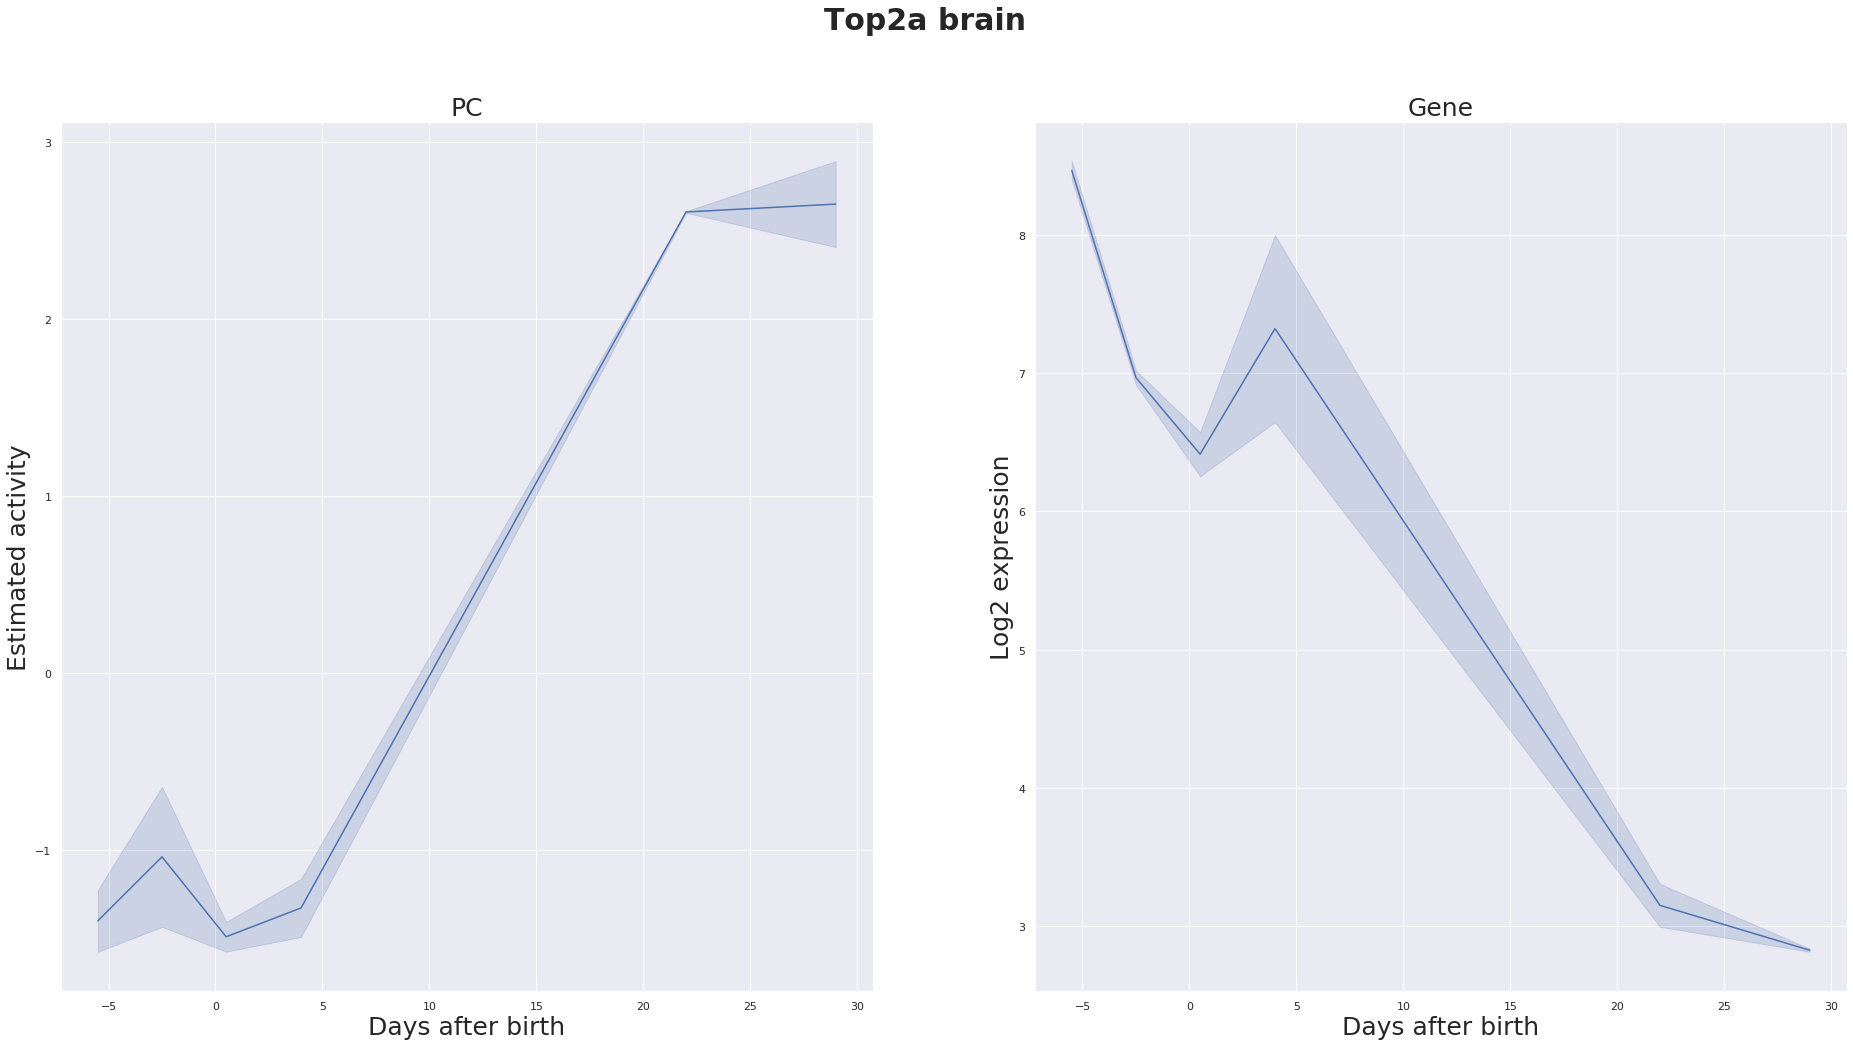
\includegraphics[width=6cm,height=3cm]{Figures&amp;Cover/Activity_Top2a_brain_NonePCremoved_filtering_False.png}
    \hspace{0.25cm}
    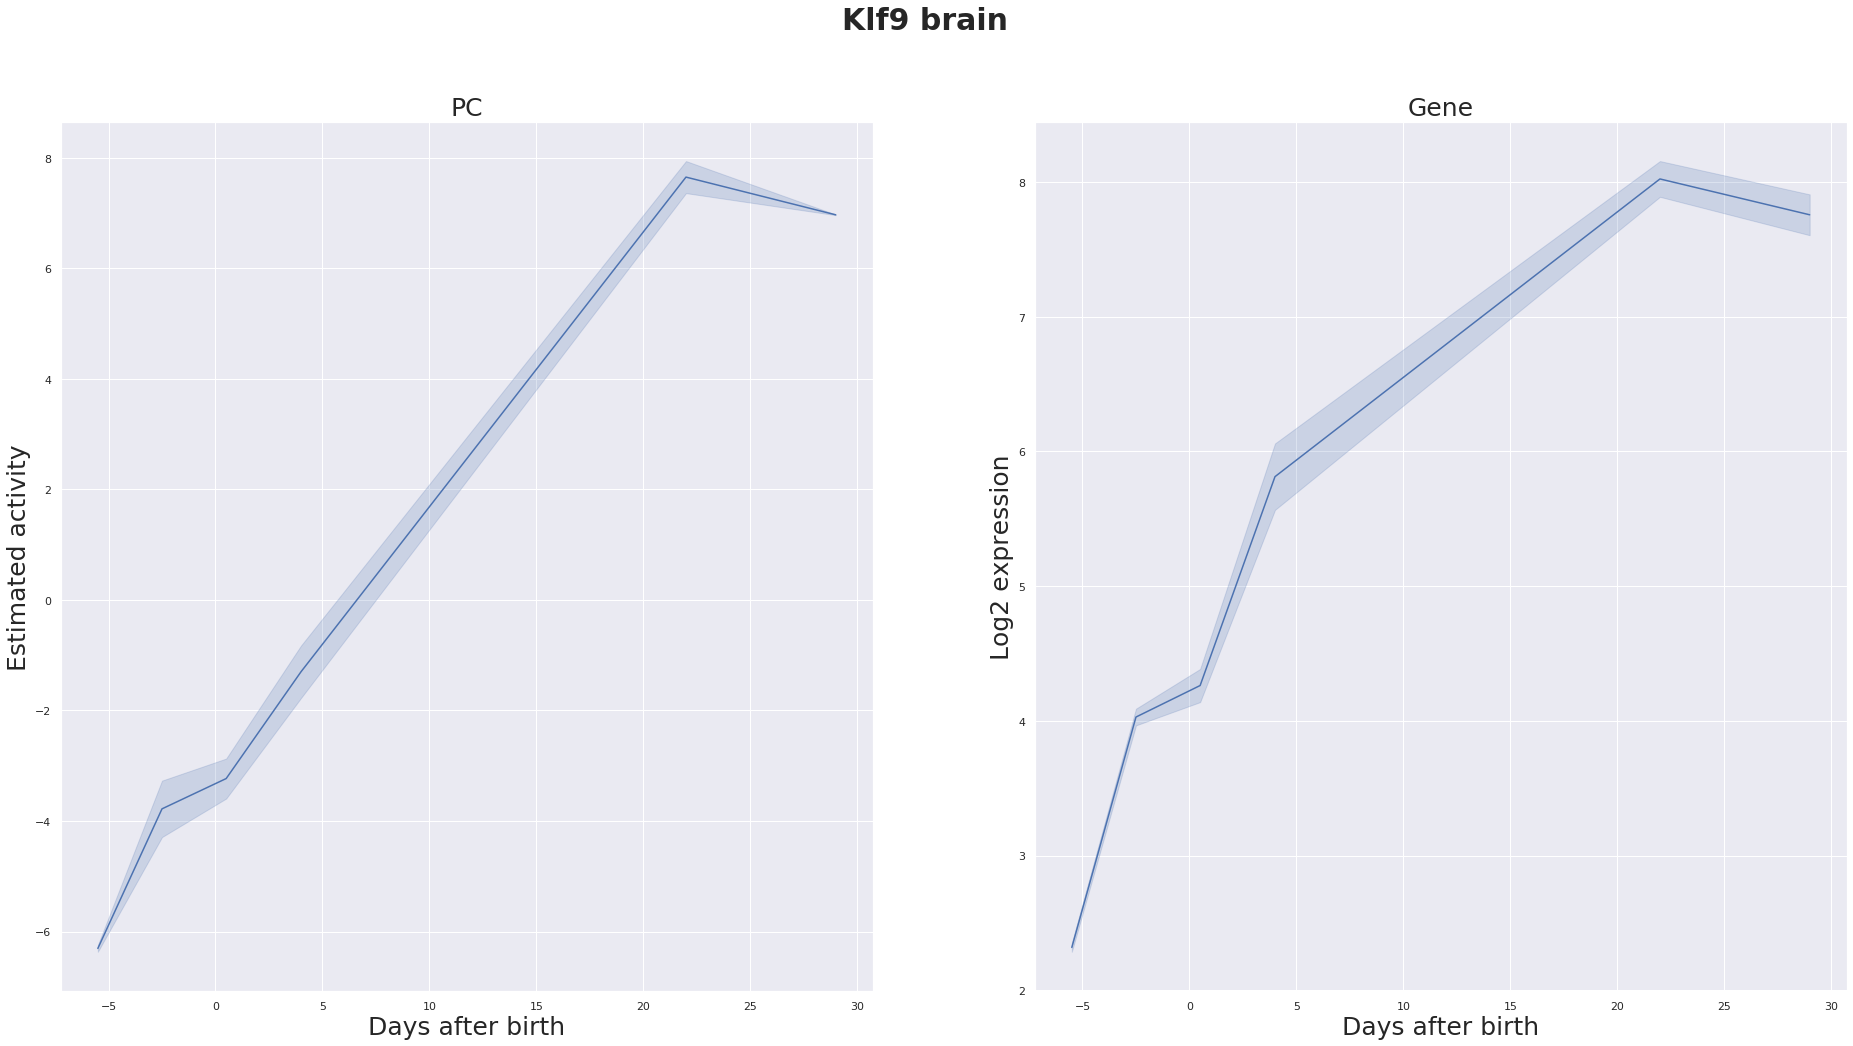
\includegraphics[width=6cm,height=3cm]{Figures&amp;Cover/Activity_Klf9_brain_NonePCremoved_filtering_False.png}
    \vspace{0.25cm}
    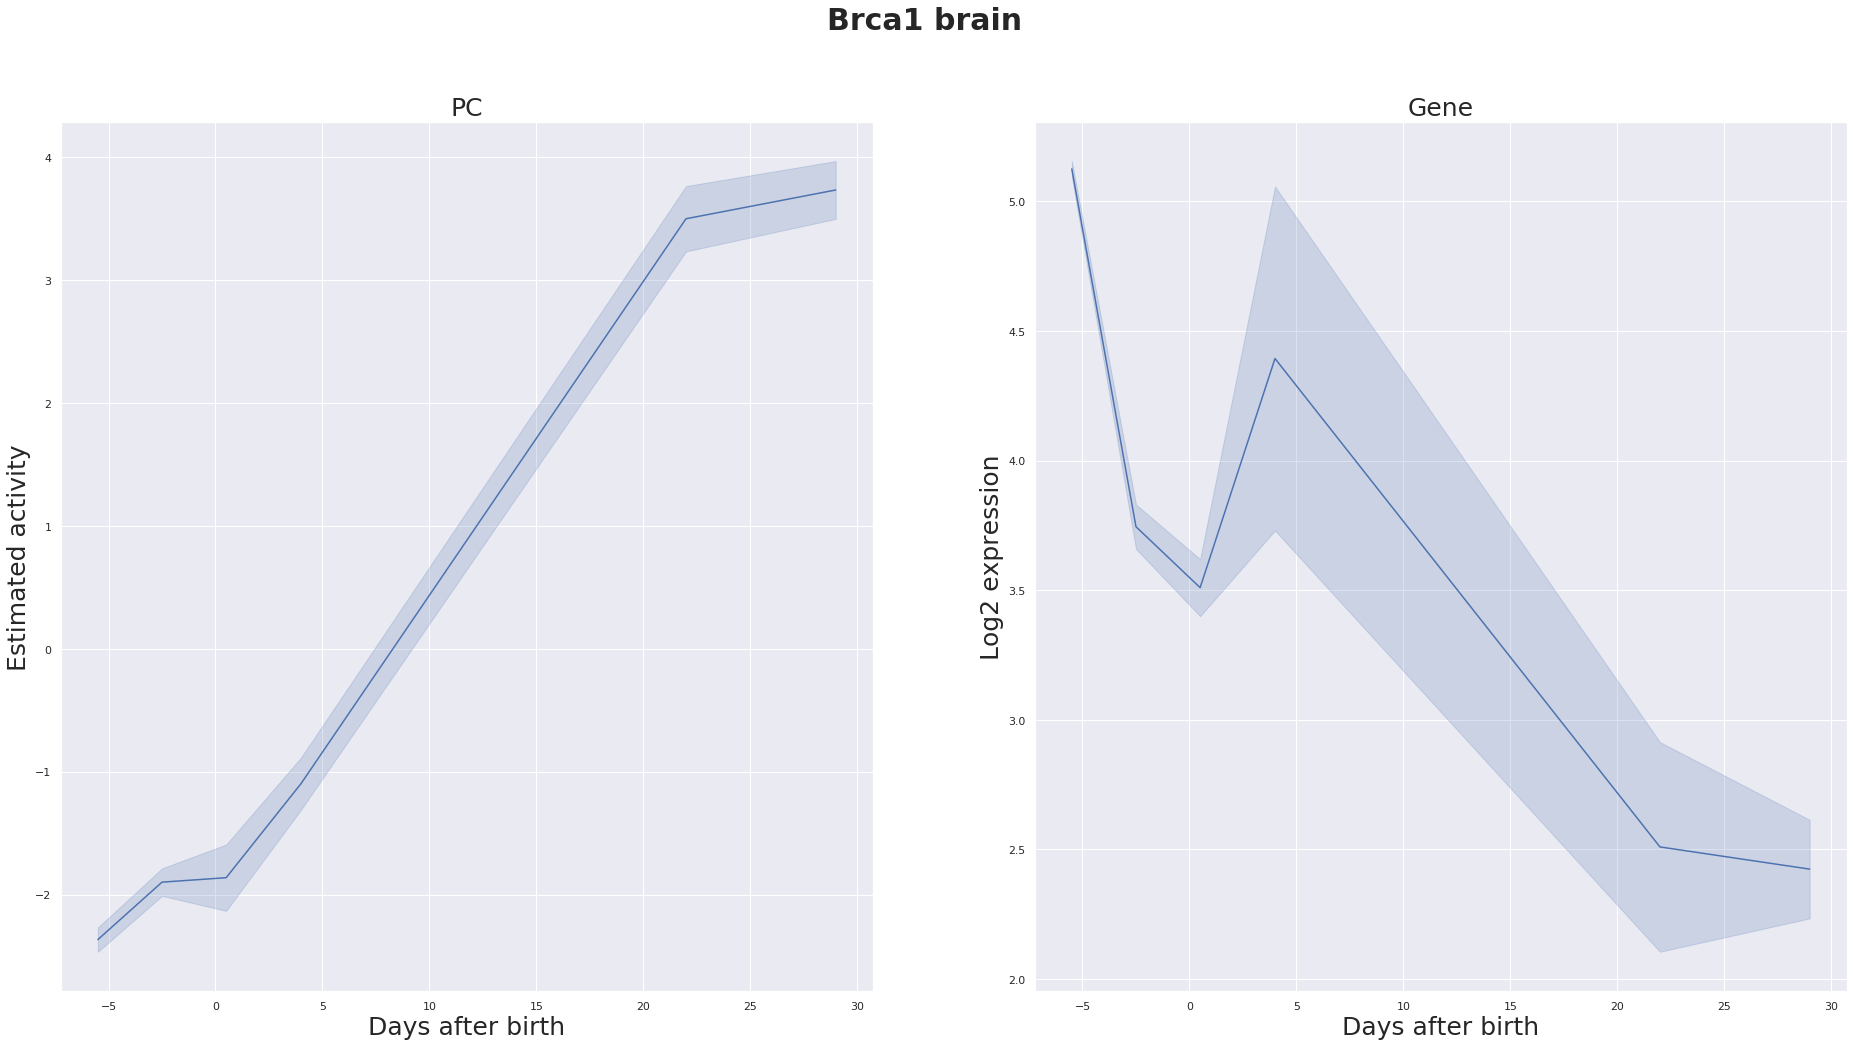
\includegraphics[width=6cm,height=3cm]{Figures&amp;Cover/Activity_Brca1_brain_NonePCremoved_filtering_False.png}
    \hspace{0.25cm}
    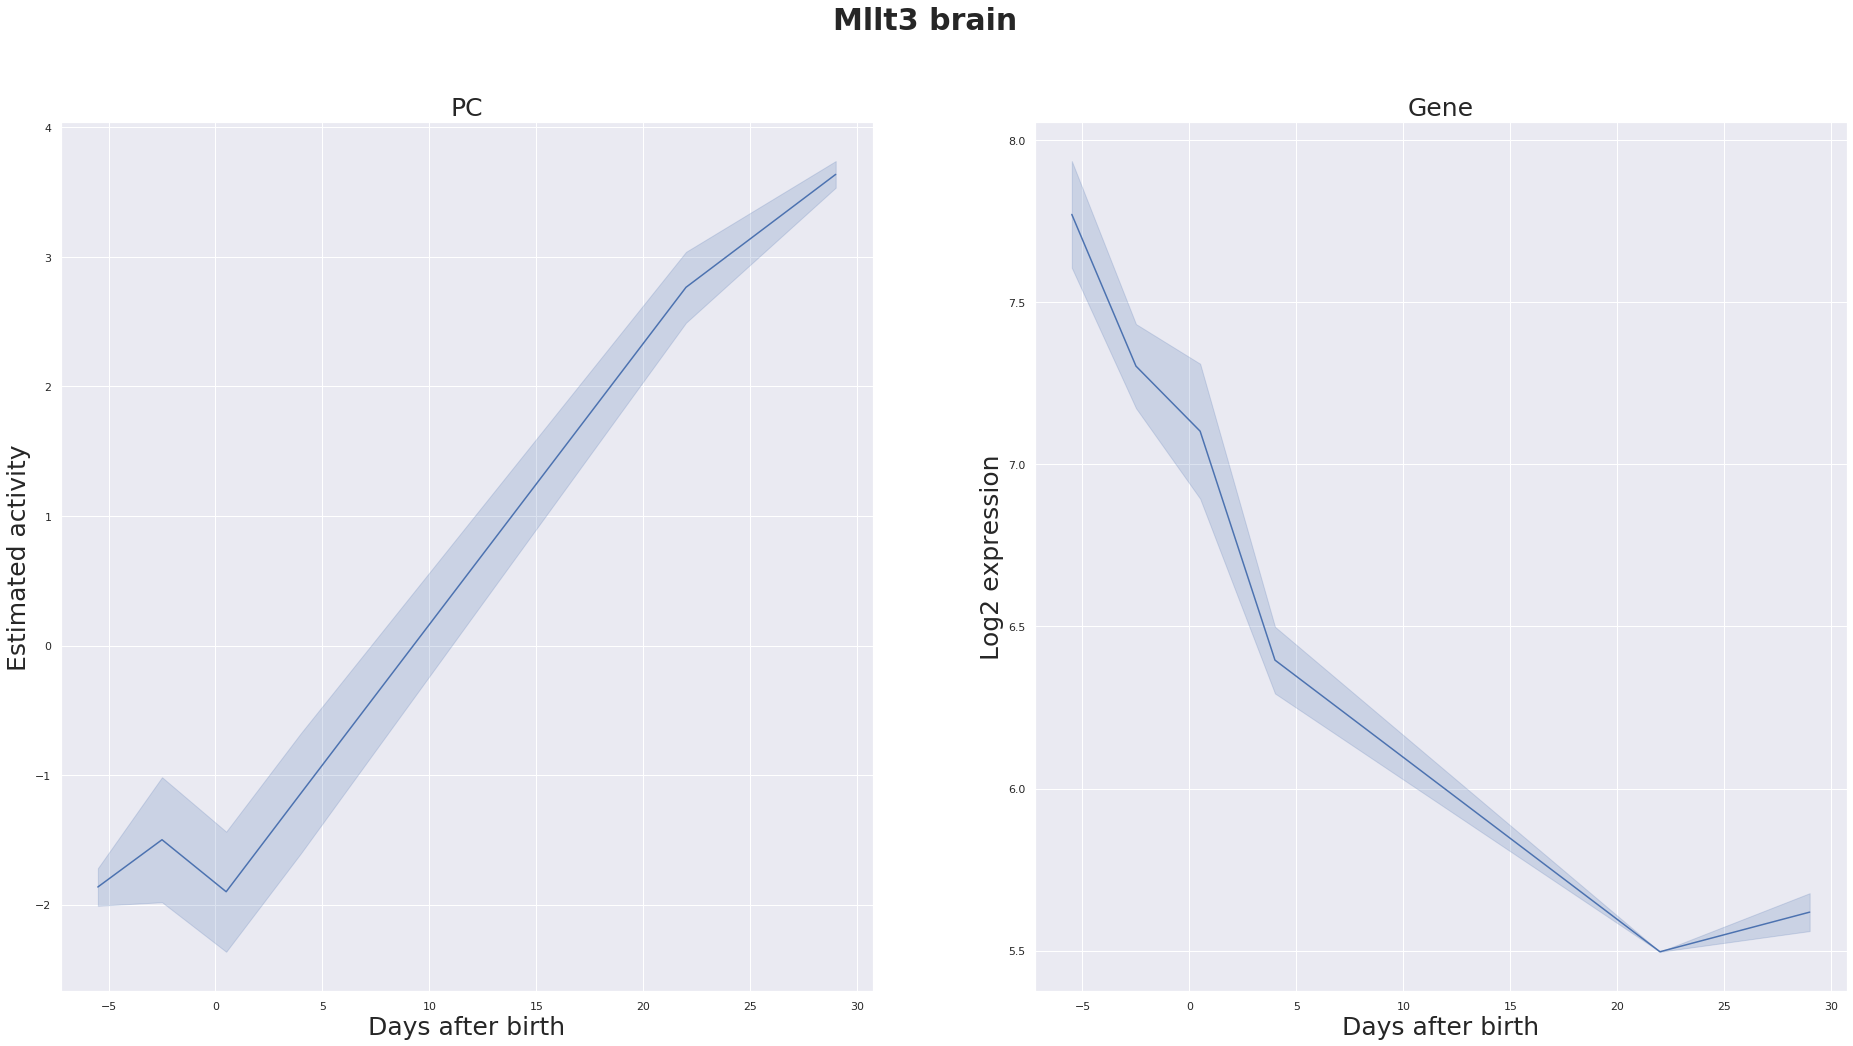
\includegraphics[width=6cm,height=3cm]{Figures&amp;Cover/Activity_Mllt3_brain_NonePCremoved_filtering_False.png}
    \vspace{0.25cm}
    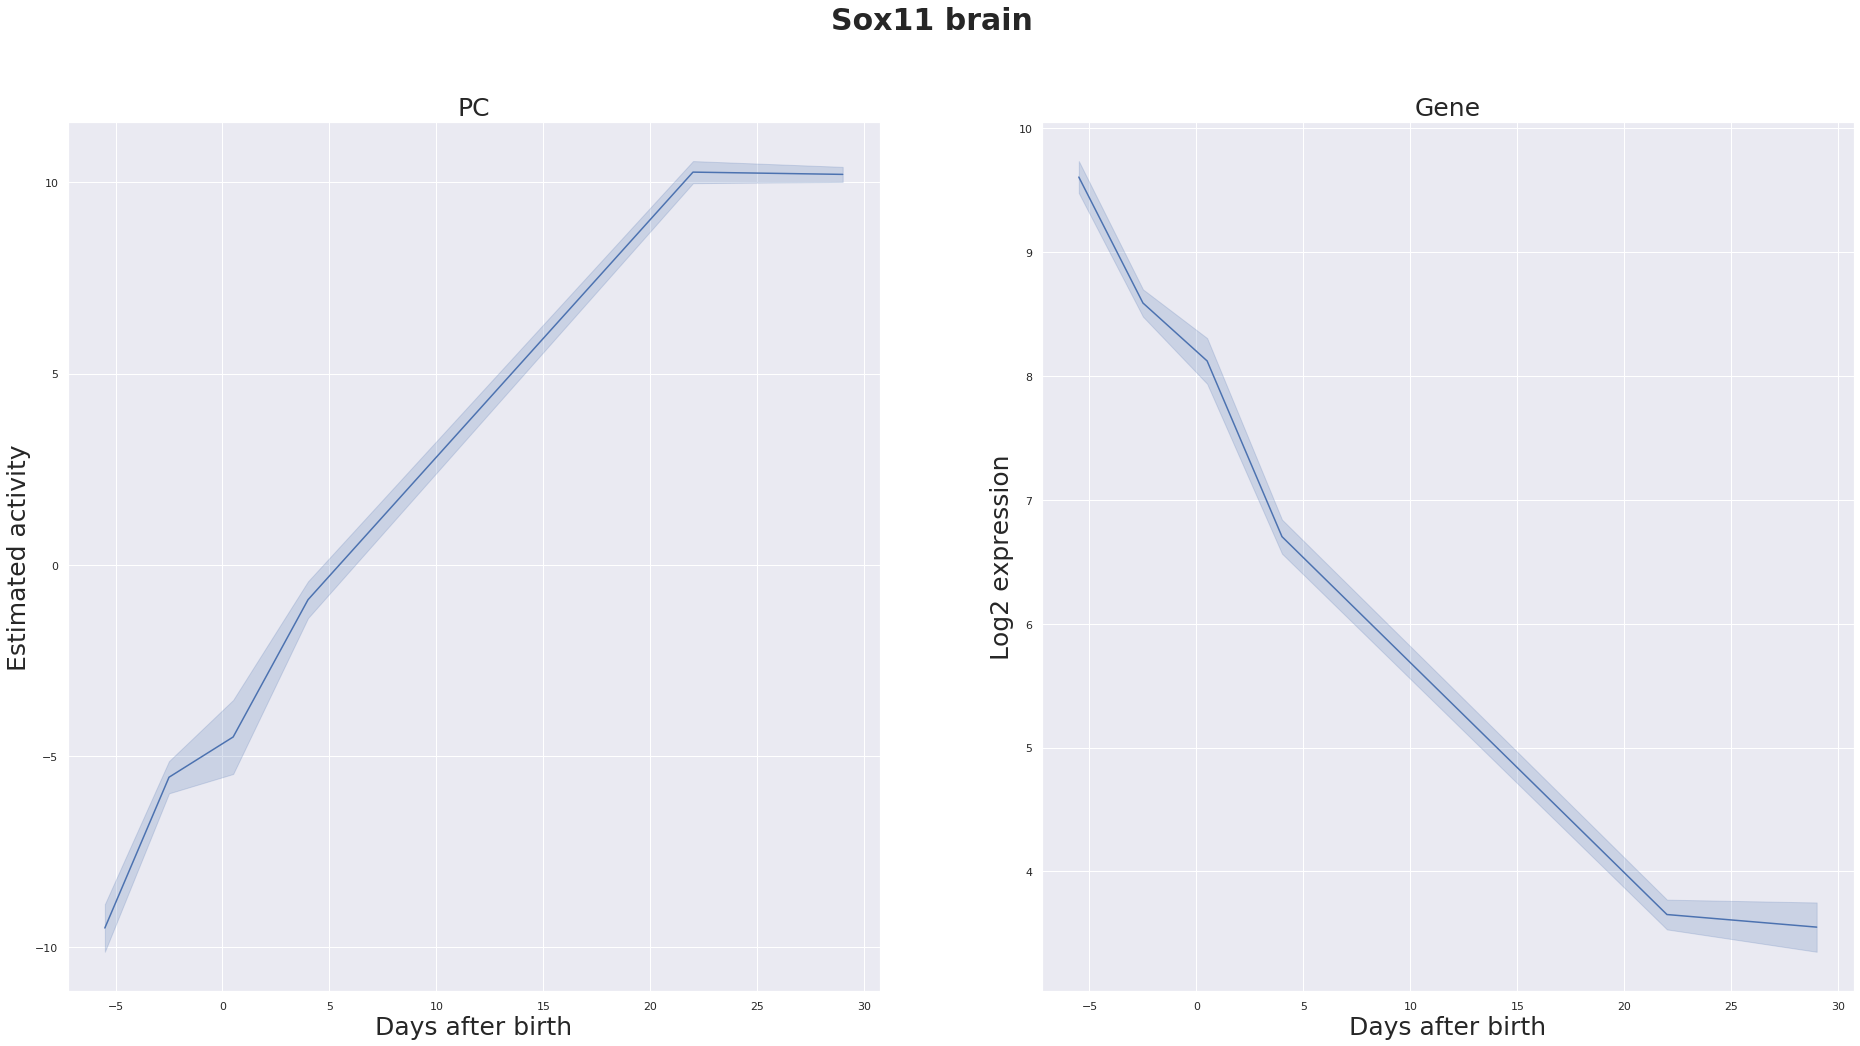
\includegraphics[width=6cm,height=3cm]{Figures&amp;Cover/Activity_Sox11_brain_NonePCremoved_filtering_False.png}
    \caption{\textbf{Estimated activities of Tal1, Lmo2, Ncapg, Ikzf1, Top2a, Klf9, Brca1, Mllt3 and Sox11 in mouse brains as a functions of the mices' age.} The activities were estimated by the first \ac{PC} of the mRNA expression data of the genes each \ac{TF} is likely to regulate (left figure of each pair) as well as directly through the transcription of the genes coding for each \ac{TF}, as log2-transformed \ac{RPM} transcript counts (right figure of each pair).}
    \label{fig:BrainEsts1}
\end{figure}    
    
\begin{figure}
    \centering
    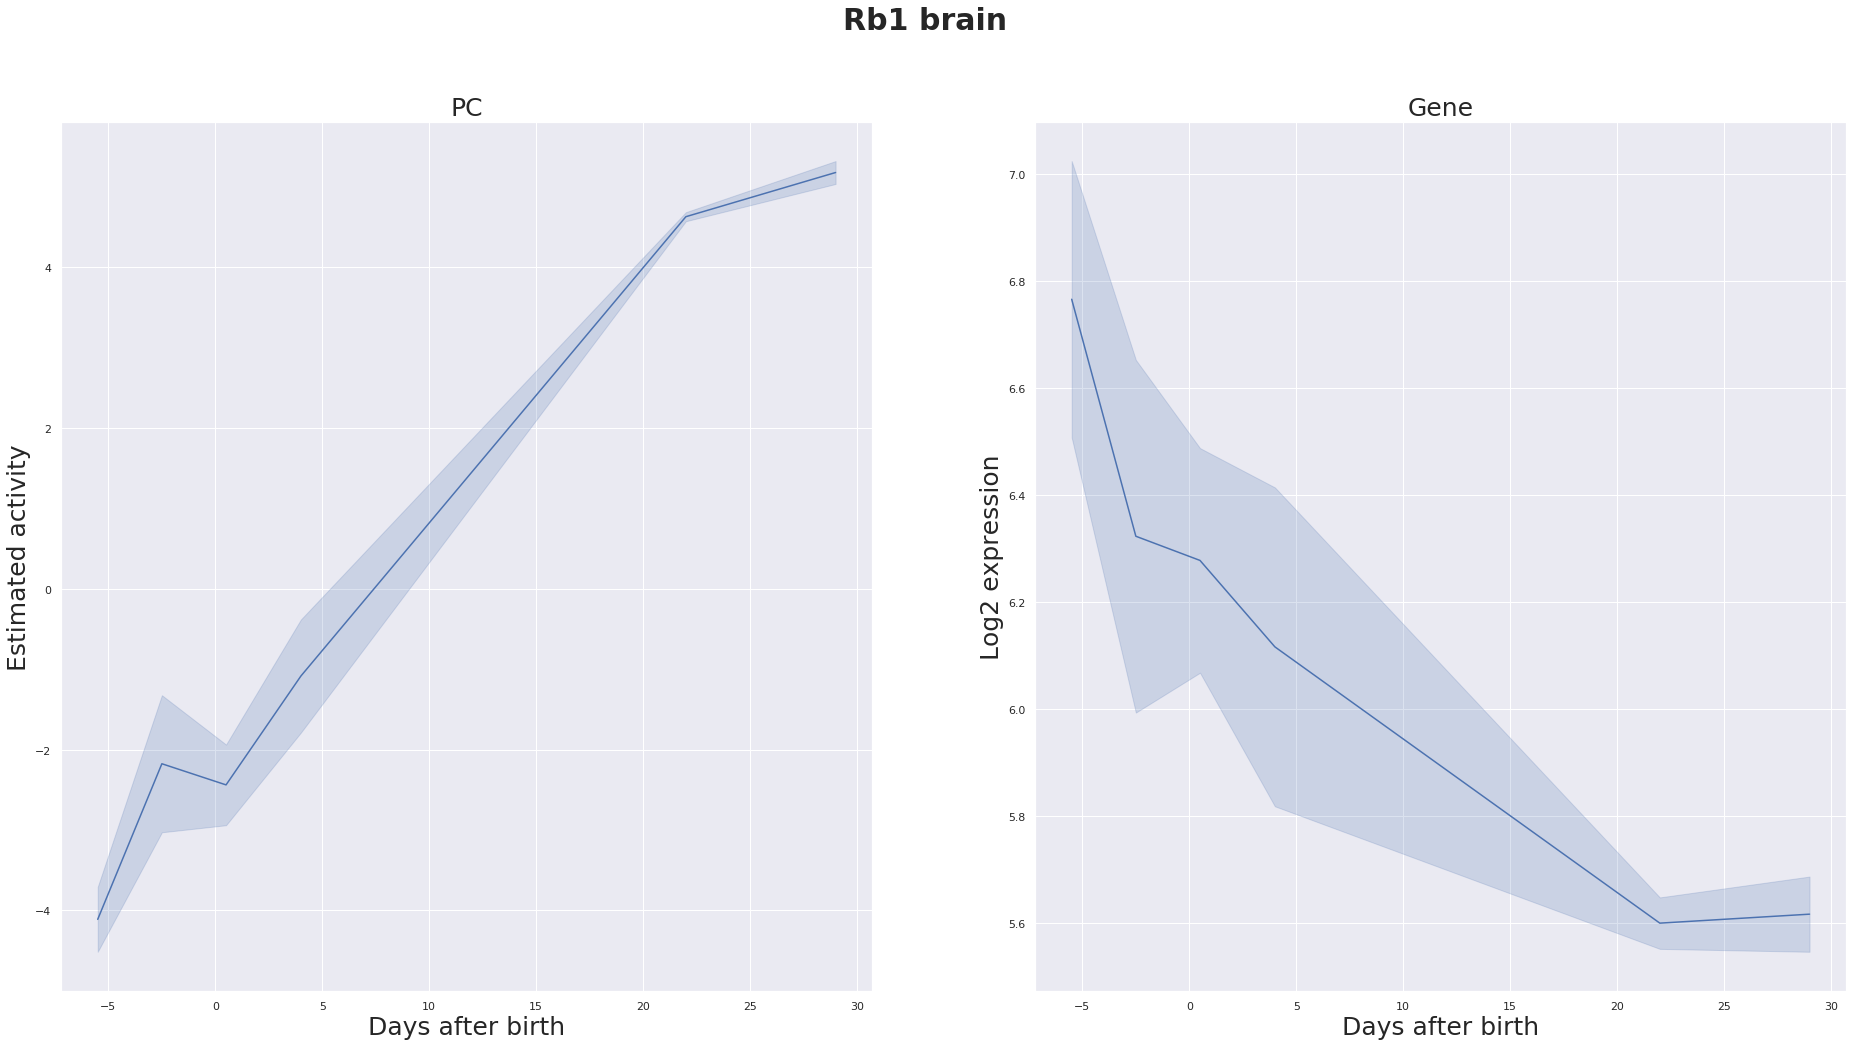
\includegraphics[width=6cm,height=3cm]{Figures&amp;Cover/Activity_Rb1_brain_NonePCremoved_filtering_False.png}
    \hspace{0.25cm}
    \vspace{0.25cm}
    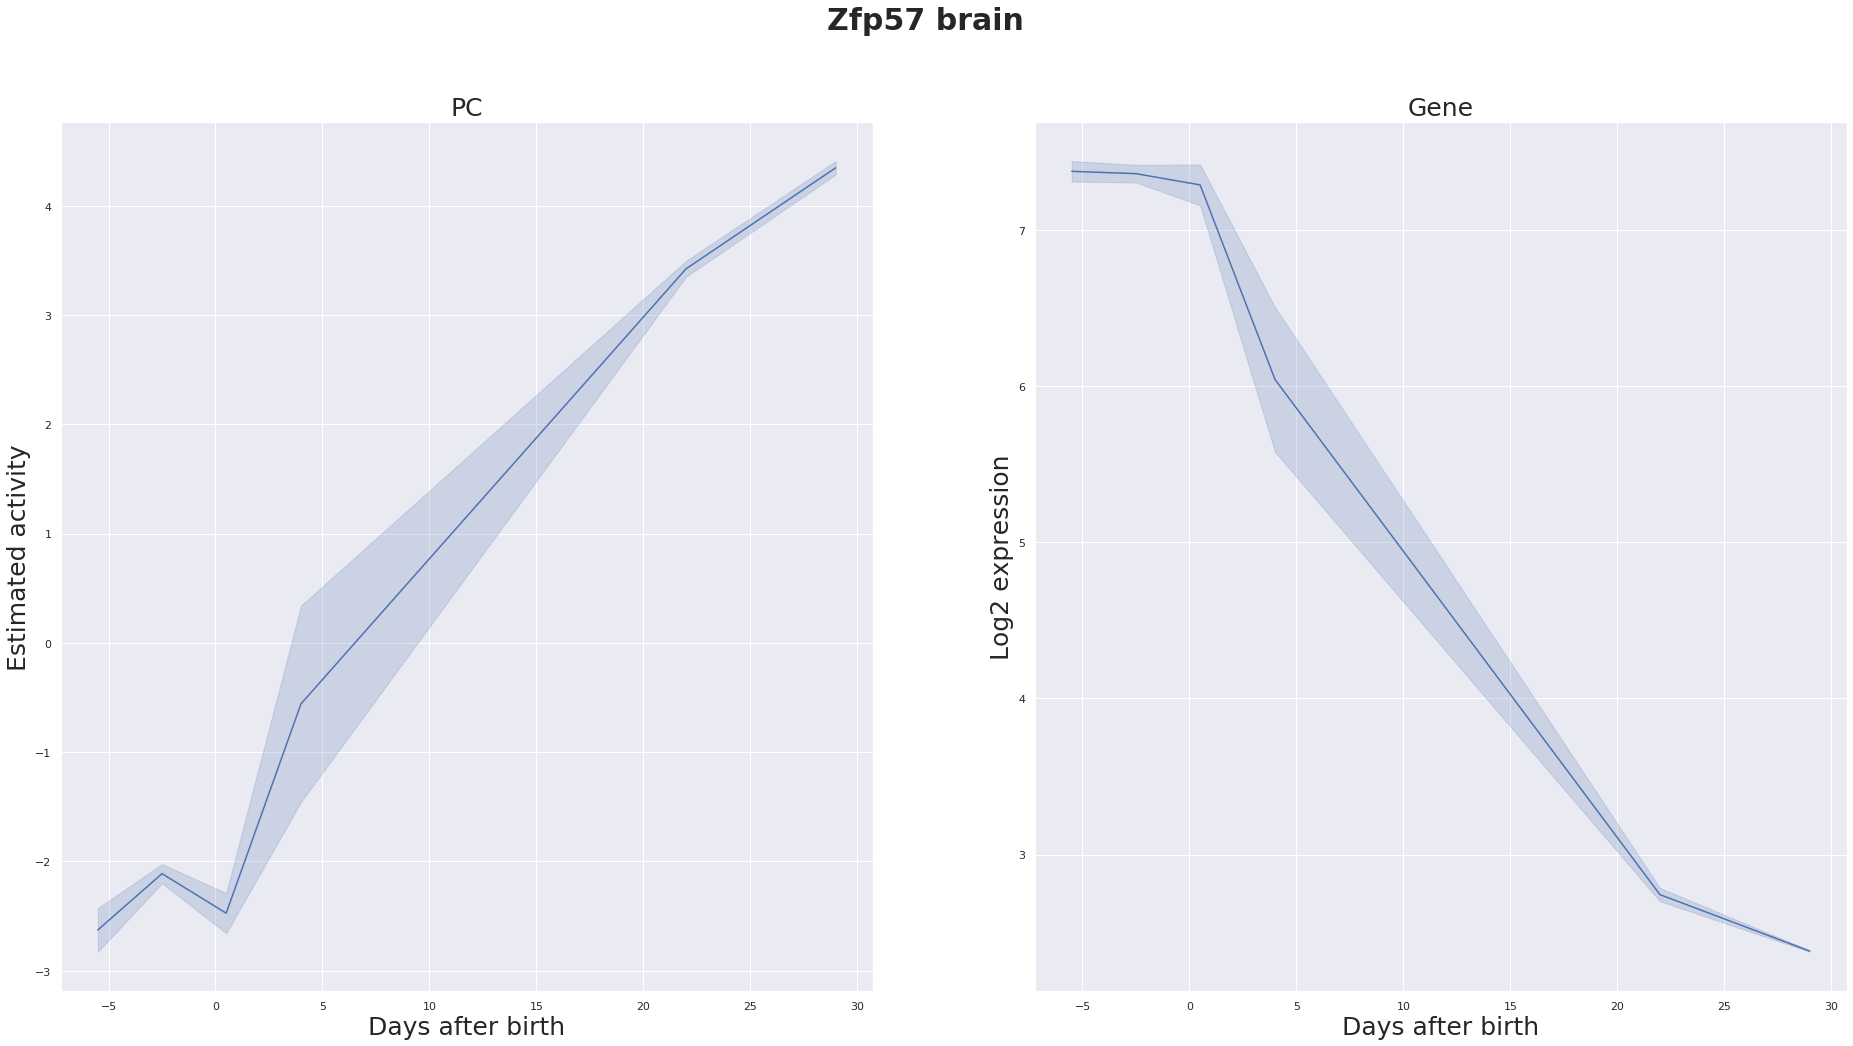
\includegraphics[width=6cm,height=3cm]{Figures&amp;Cover/Activity_Zfp57_brain_NonePCremoved_filtering_False.png}
    \vspace{0.25cm}
    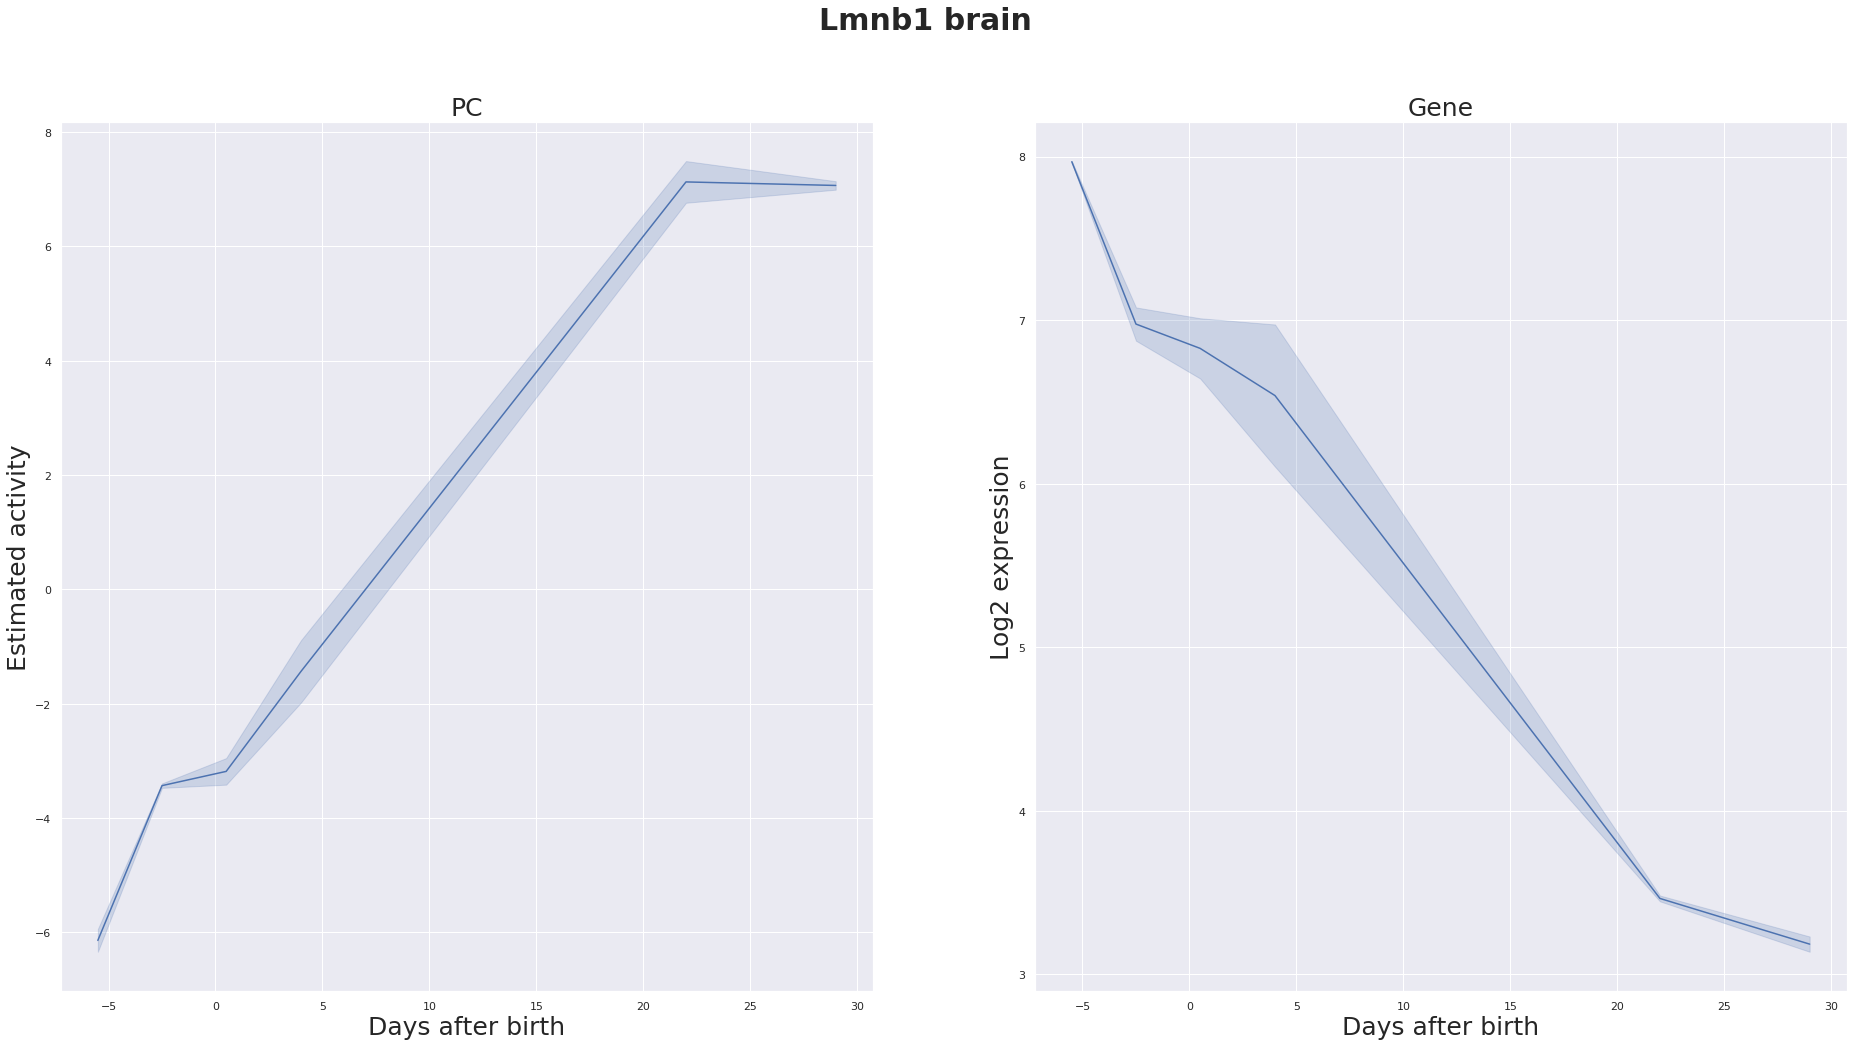
\includegraphics[width=6cm,height=3cm]{Figures&amp;Cover/Activity_Lmnb1_brain_NonePCremoved_filtering_False.png}
    \hspace{0.25cm}
    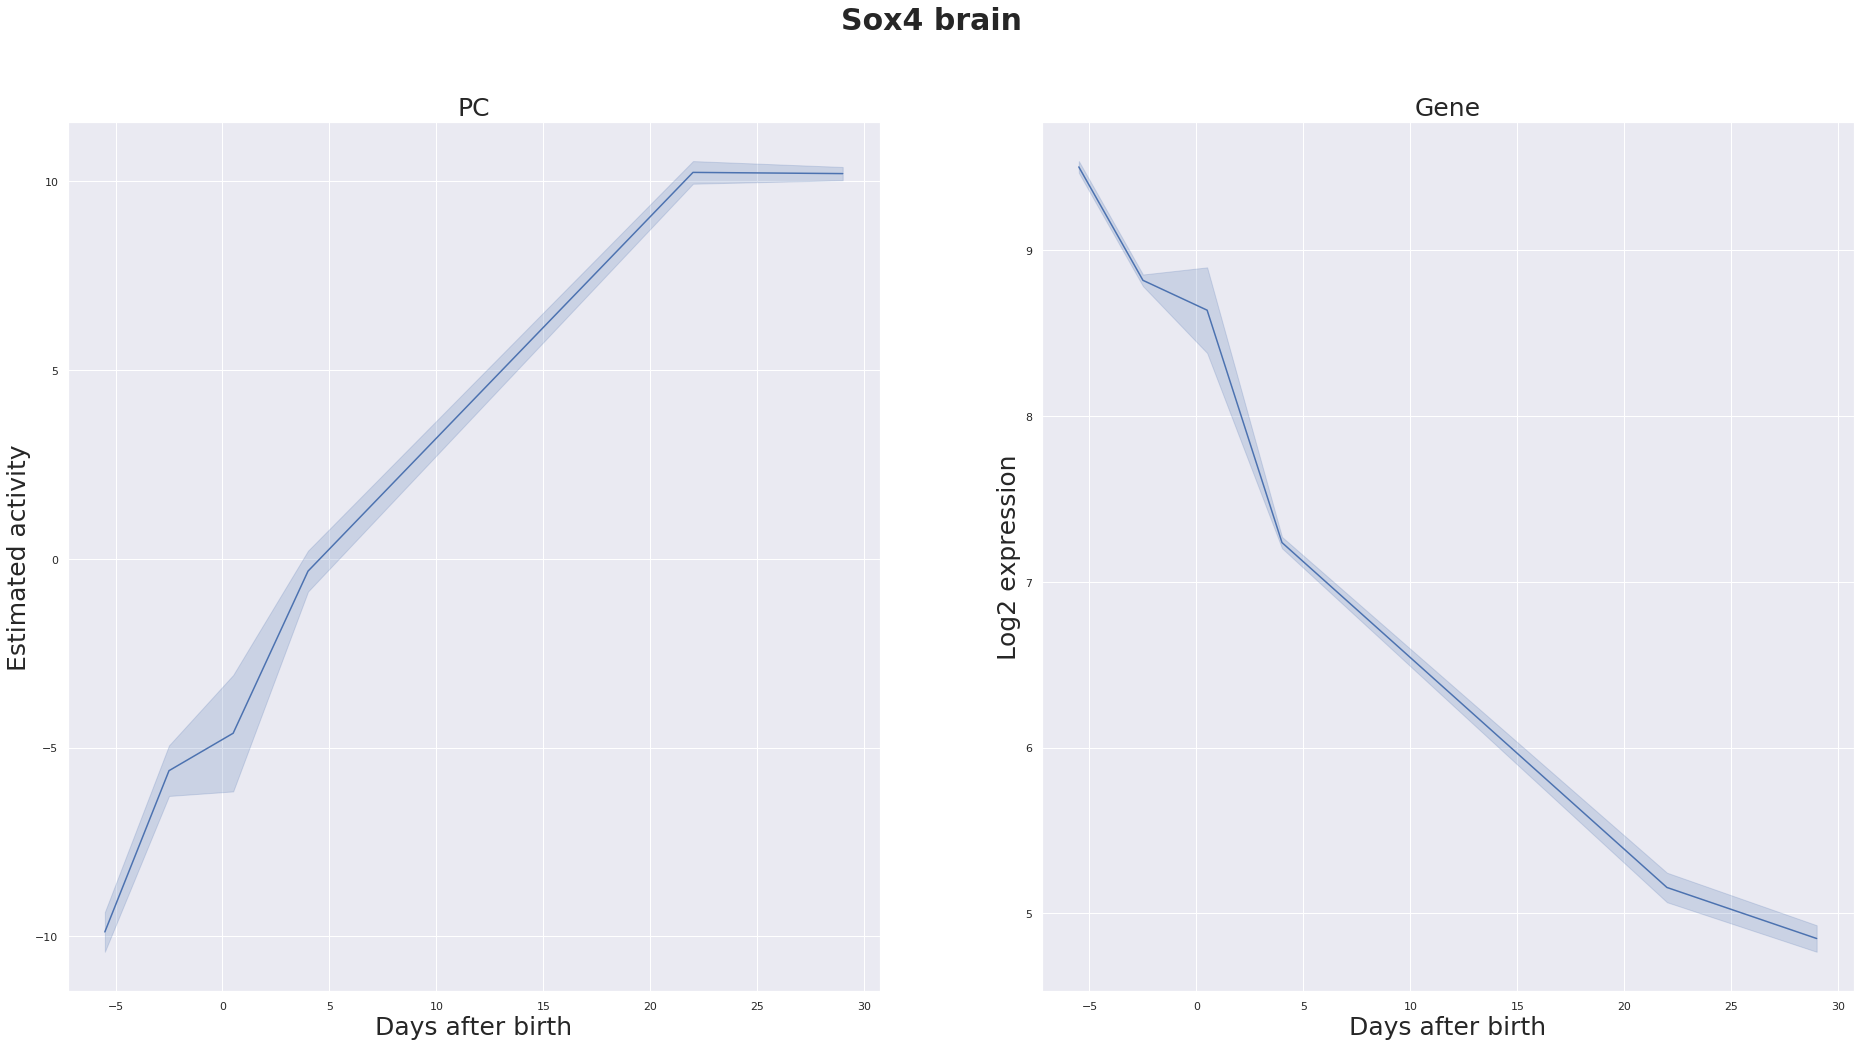
\includegraphics[width=6cm,height=3cm]{Figures&amp;Cover/Activity_Sox4_brain_NonePCremoved_filtering_False.png}
    \vspace{0.25cm}
    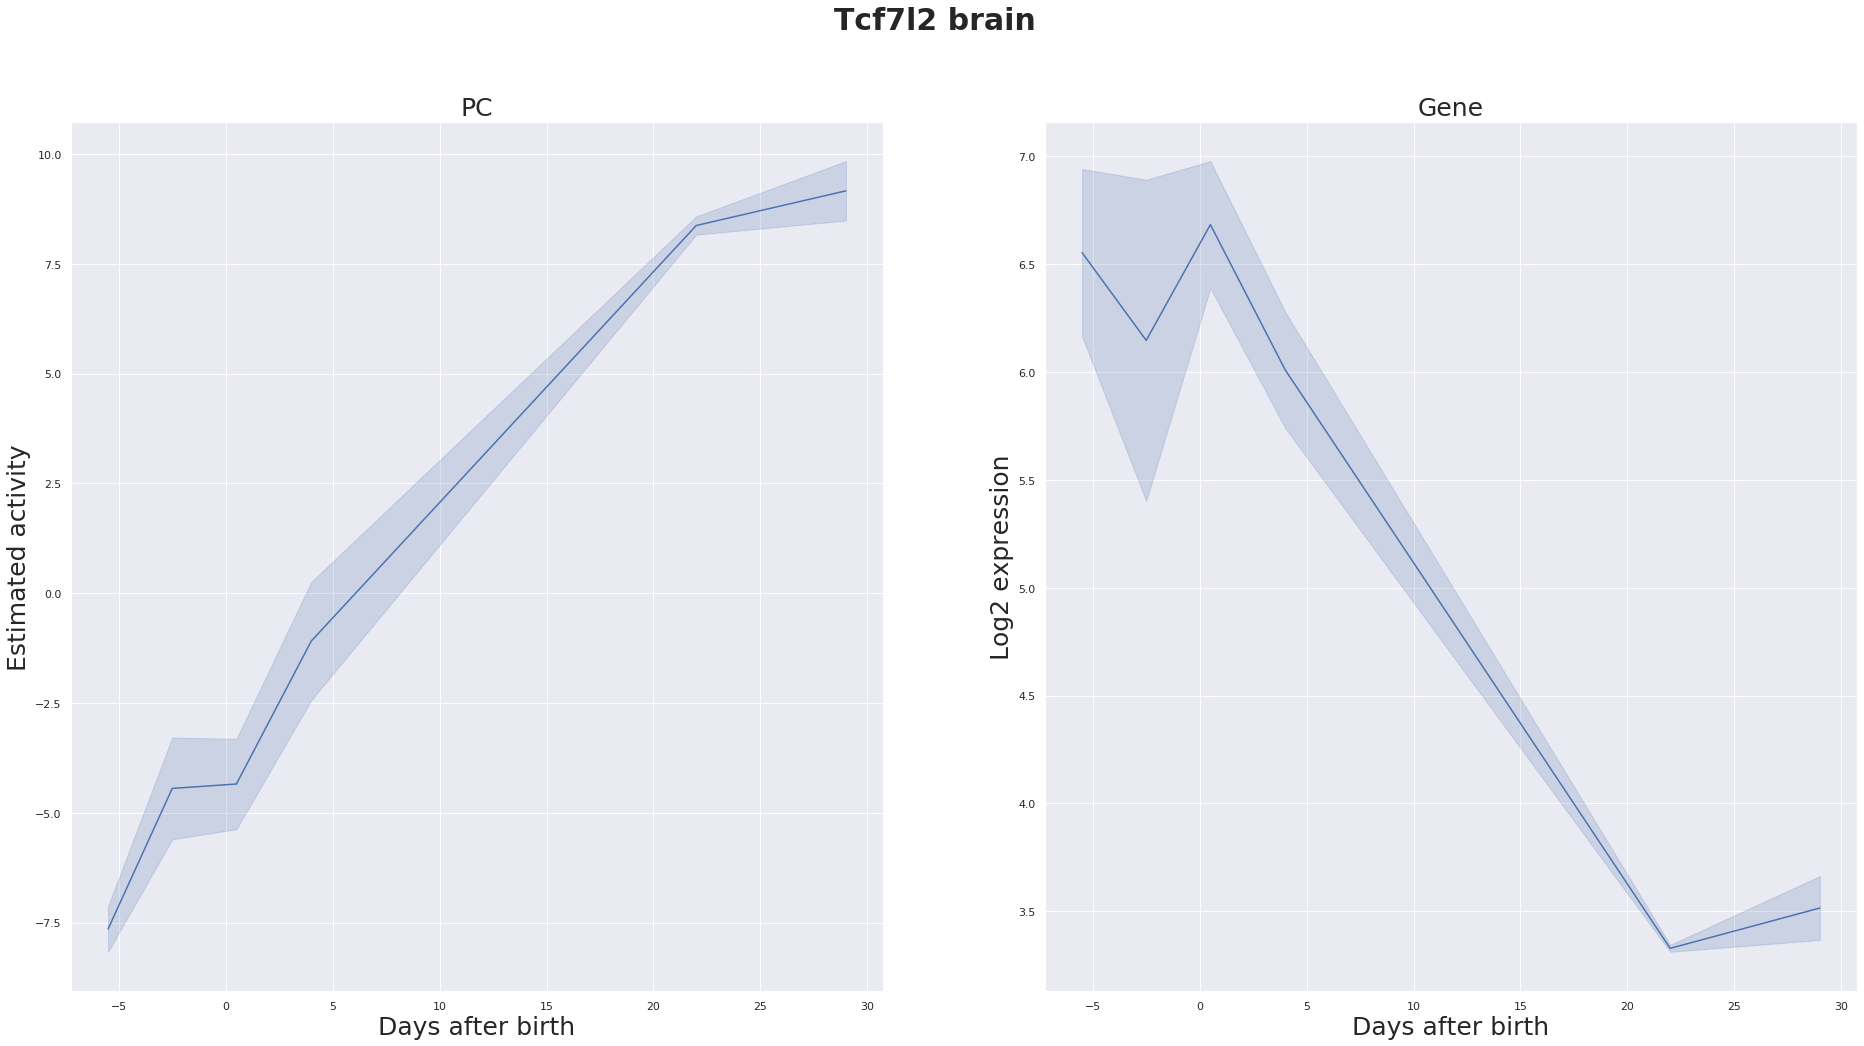
\includegraphics[width=6cm,height=3cm]{Figures&amp;Cover/Activity_Tcf7l2_brain_NonePCremoved_filtering_False.png}
    \hspace{0.25cm}
    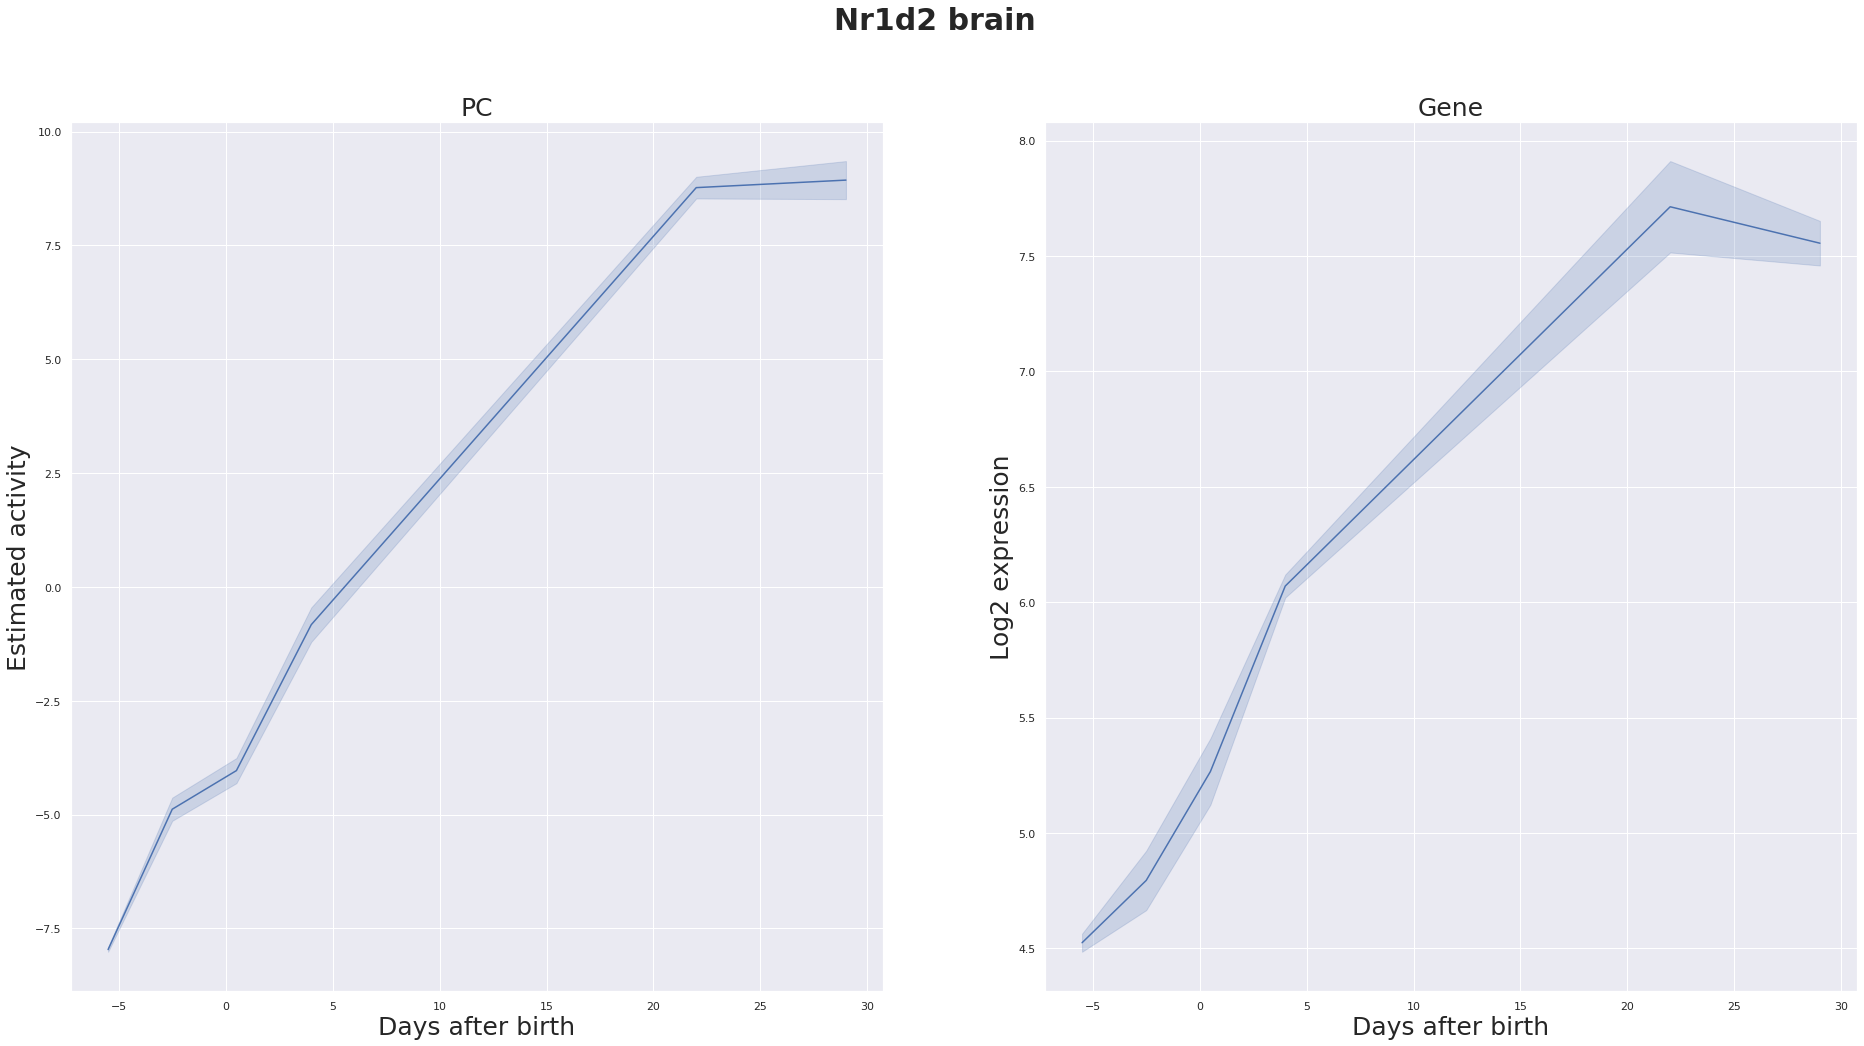
\includegraphics[width=6cm,height=3cm]{Figures&amp;Cover/Activity_Nr1d2_brain_NonePCremoved_filtering_False.png}
    \vspace{0.25cm}
    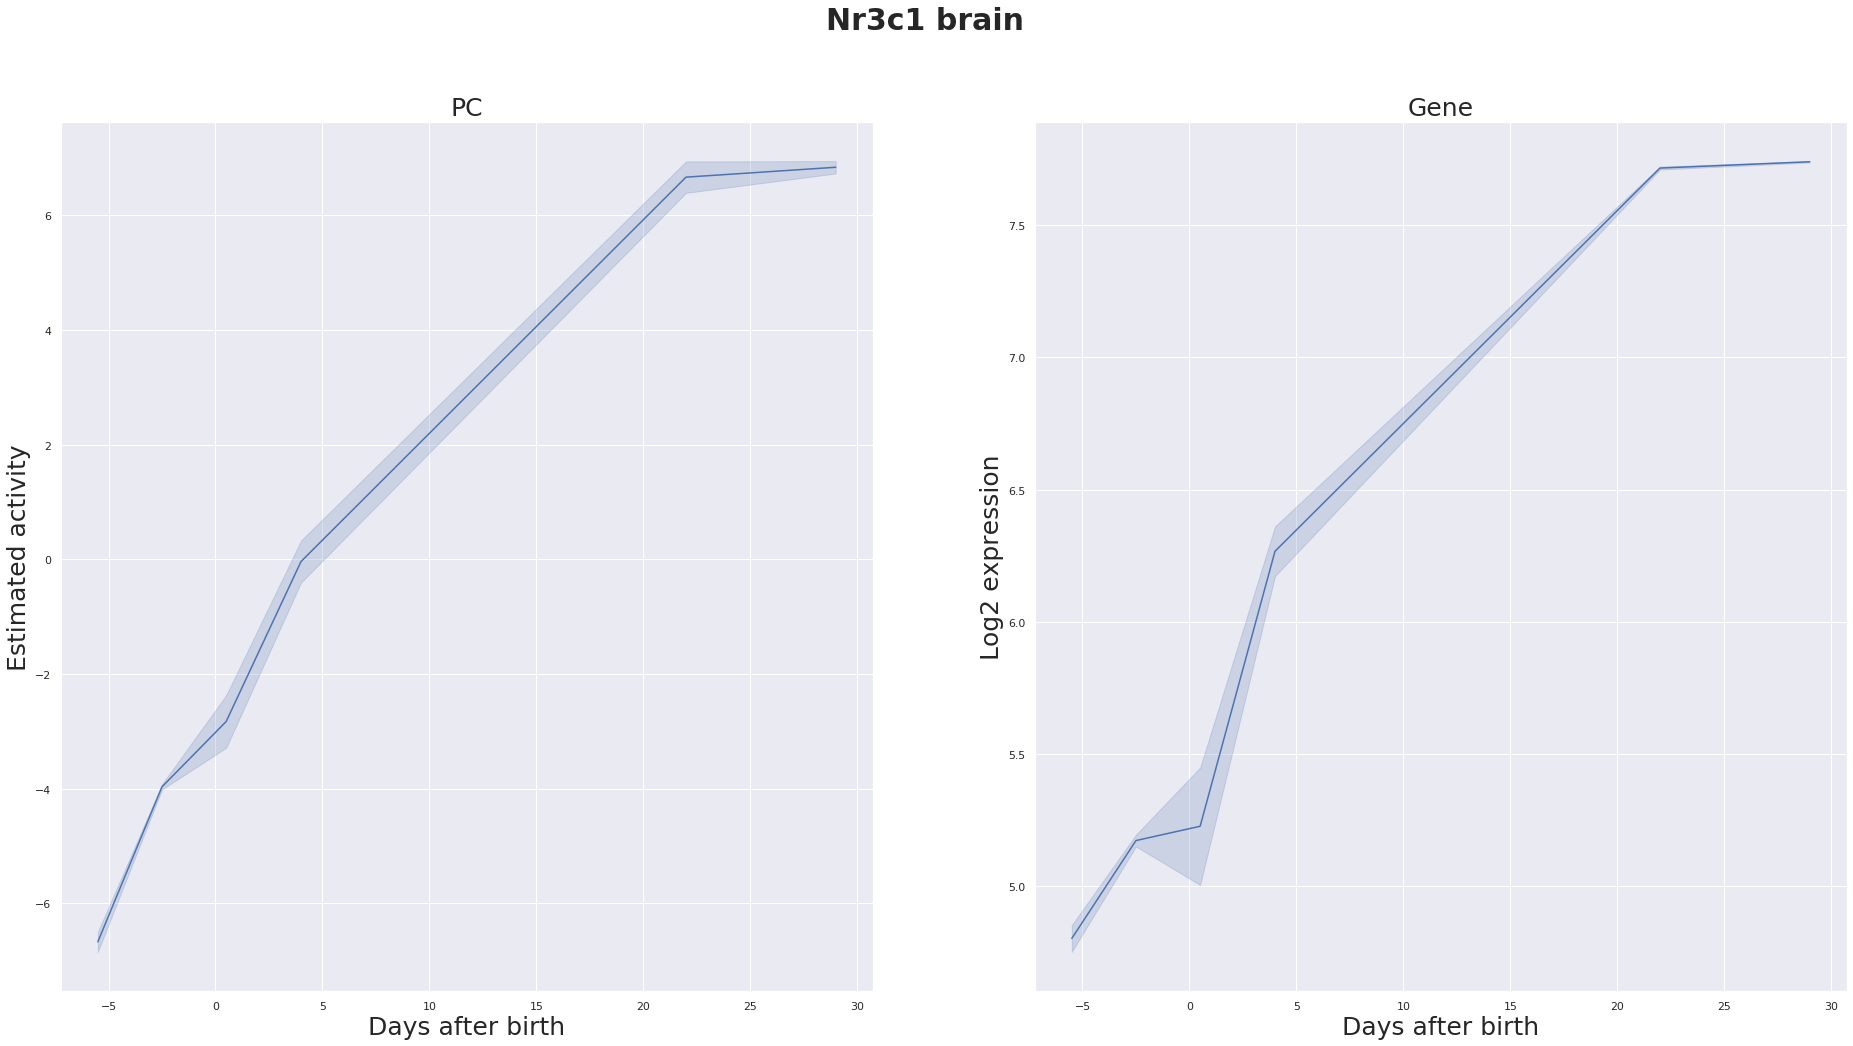
\includegraphics[width=6cm,height=3cm]{Figures&amp;Cover/Activity_Nr3c1_brain_NonePCremoved_filtering_False.png}
    \hspace{0.25cm}
    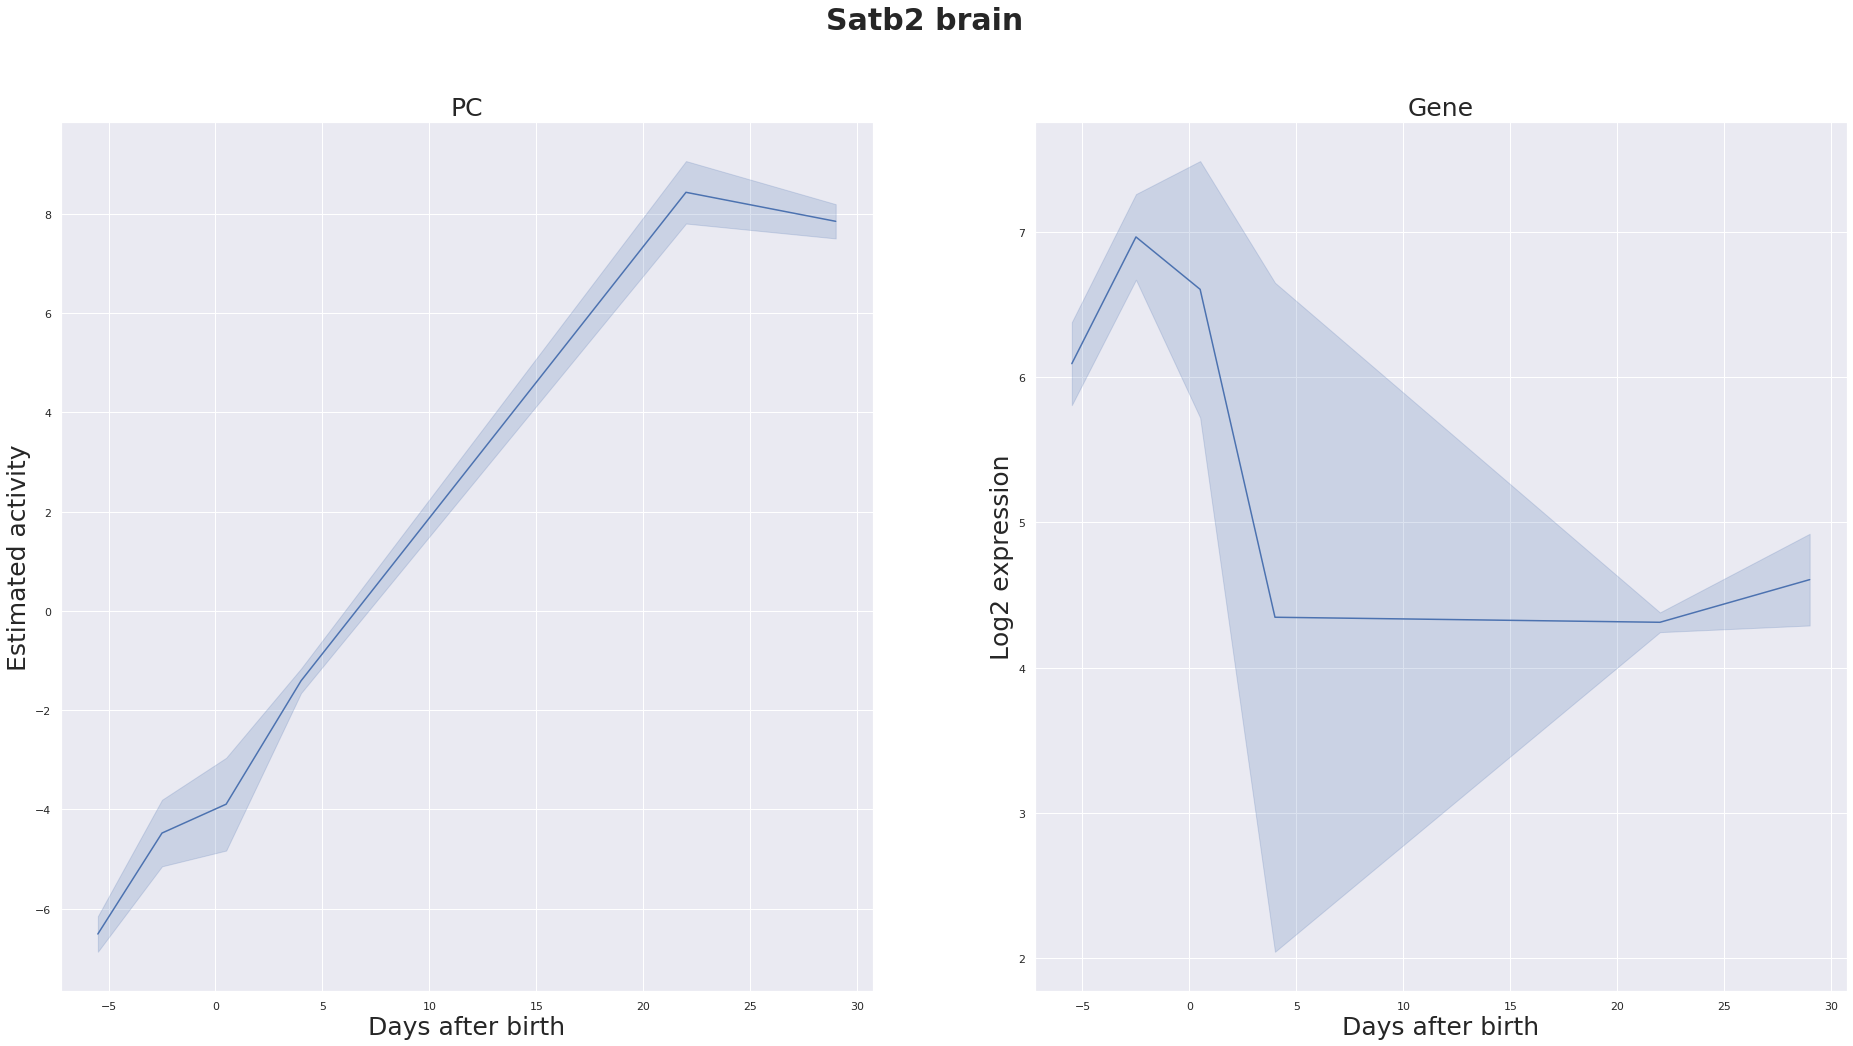
\includegraphics[width=6cm,height=3cm]{Figures&amp;Cover/Activity_Satb2_brain_NonePCremoved_filtering_False.png}
    \caption{\textbf{Estimated activities of Rb1, Zfp57, Lmnb1, Sox4, Tc7l2, Nr1d2, Nr3c1 and Satb2 in mouse brains as a functions of the mices' age.} The activities were estimated by the first \ac{PC} of the mRNA expression data of the genes each \ac{TF} is likely to regulate (left figure of each pair) as well as directly through the transcription of the genes coding for each \ac{TF}, as log2-transformed \ac{RPM} transcript counts (right figure of each pair).}
    \label{fig:BrainEsts2}
\end{figure}

\begin{figure}
    \centering
    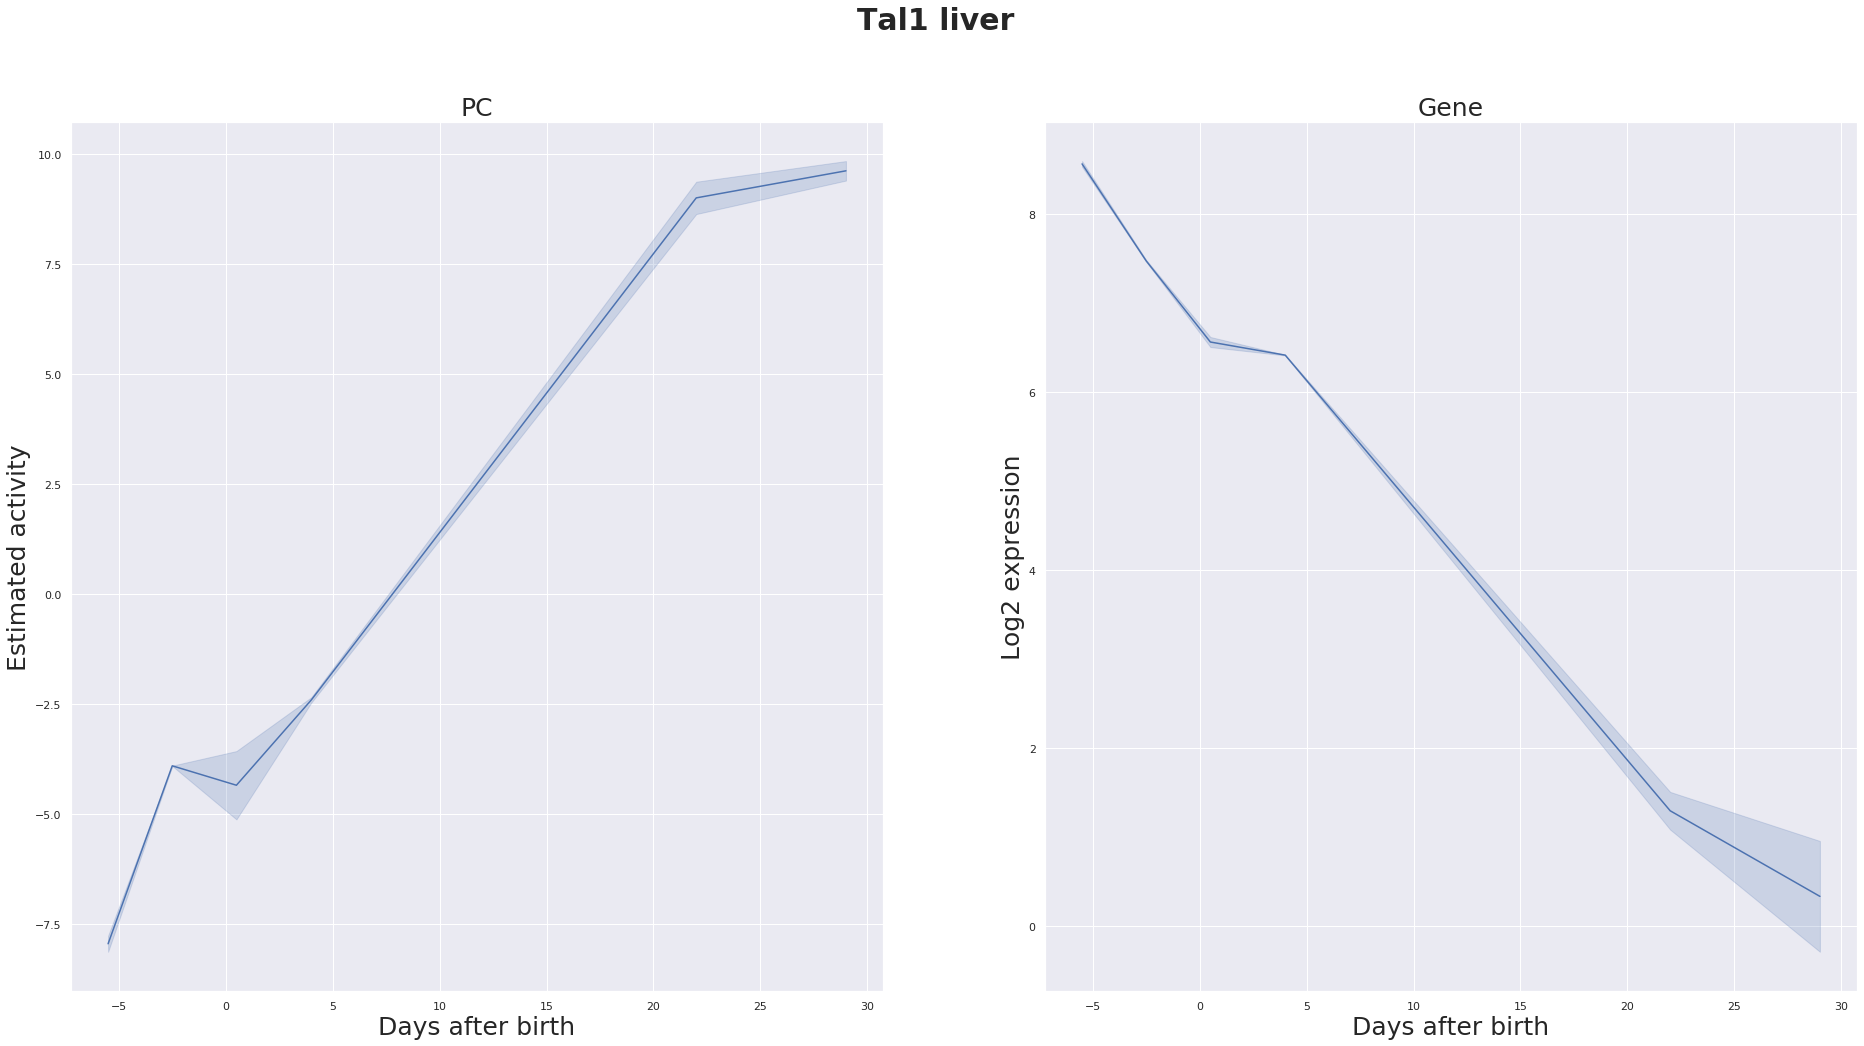
\includegraphics[width=6cm,height=3cm]{Figures&amp;Cover/Activity_Tal1_liver_NonePCremoved_filtering_False.png}
    \hspace{0.25cm}
    \vspace{0.25cm}
    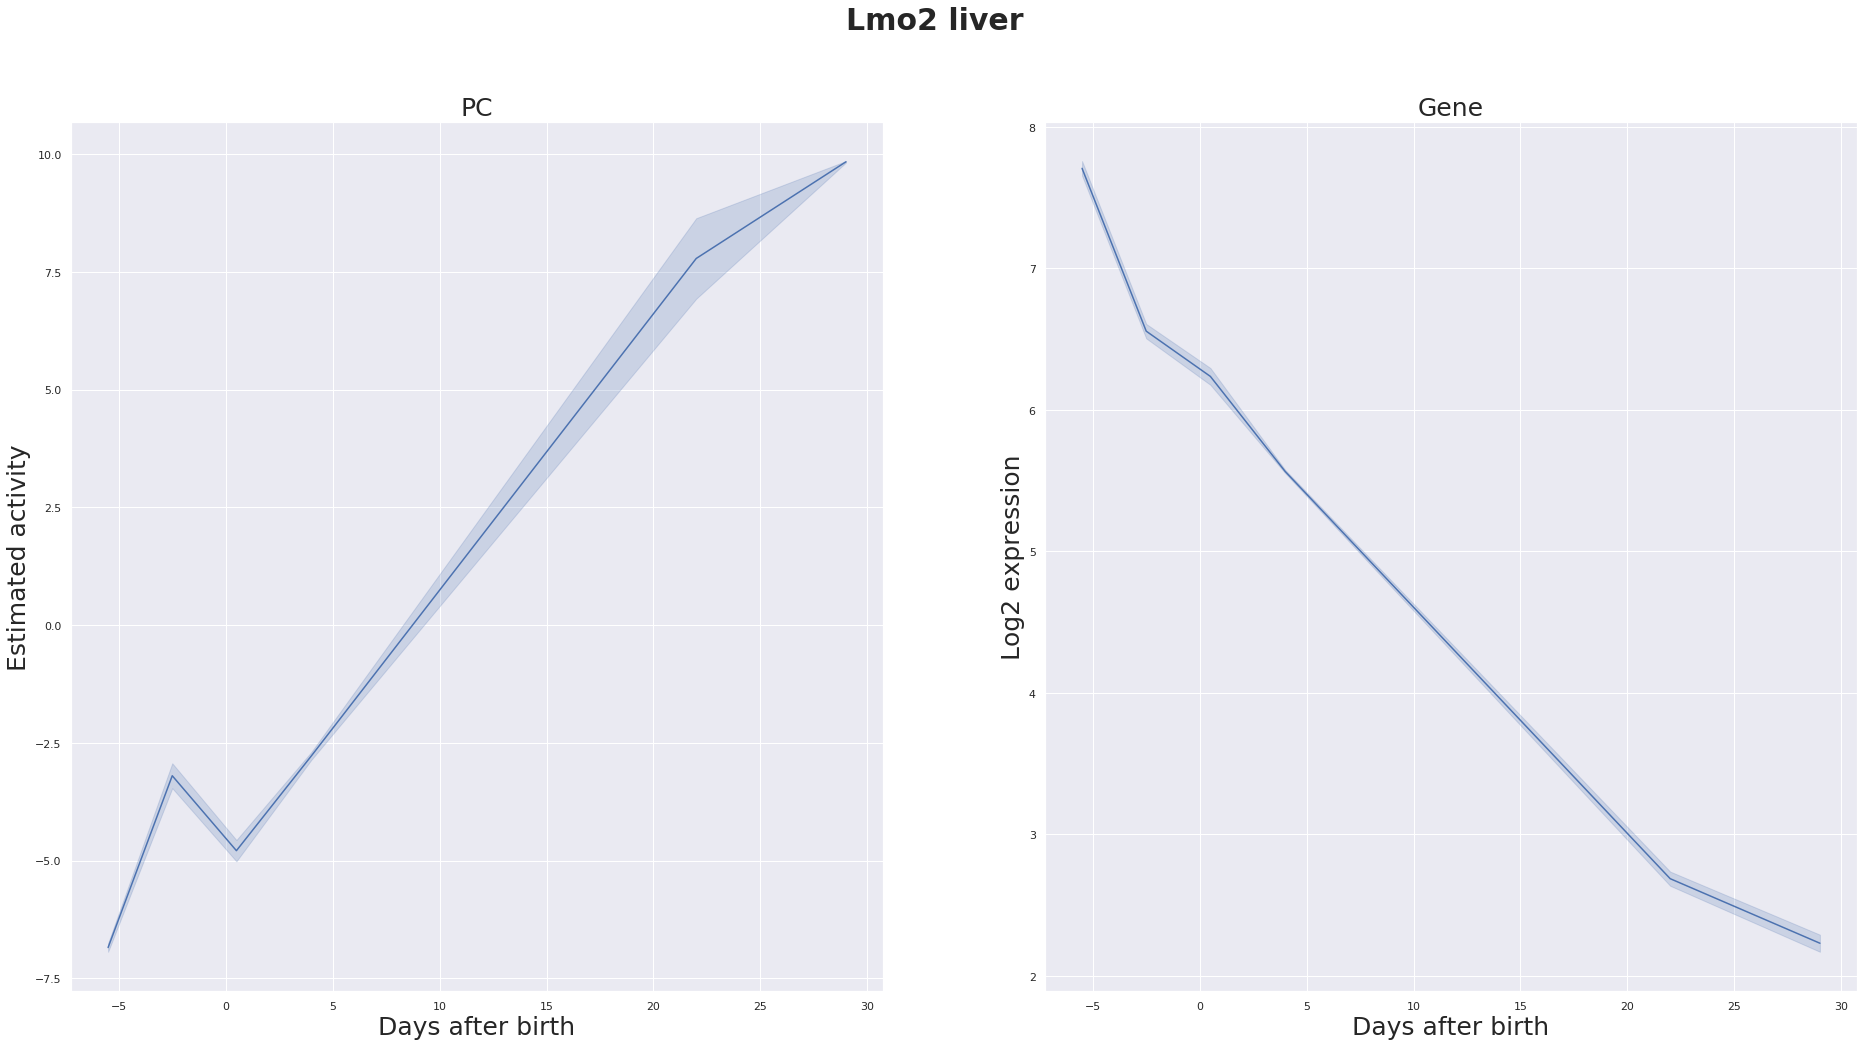
\includegraphics[width=6cm,height=3cm]{Figures&amp;Cover/Activity_Lmo2_liver_NonePCremoved_filtering_False.png}
    \vspace{0.25cm}
    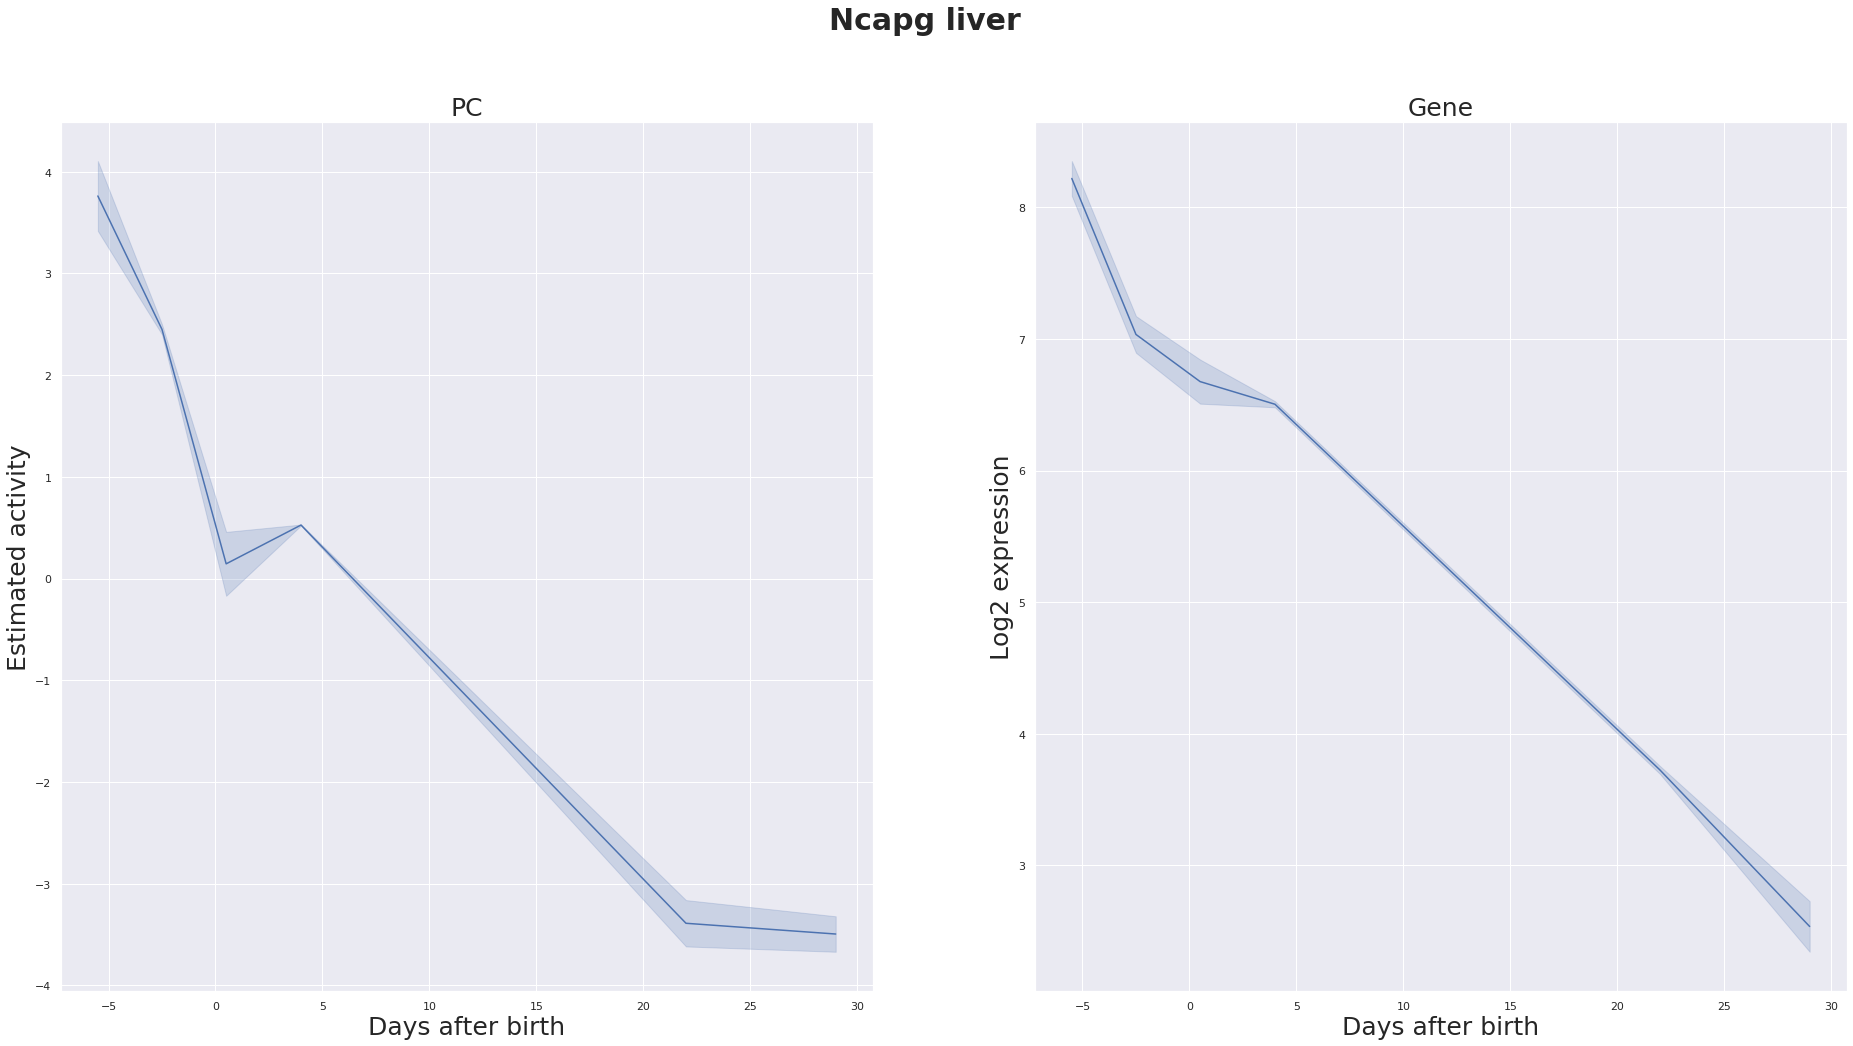
\includegraphics[width=6cm,height=3cm]{Figures&amp;Cover/Activity_Ncapg_liver_NonePCremoved_filtering_False.png}
    \hspace{0.25cm}
    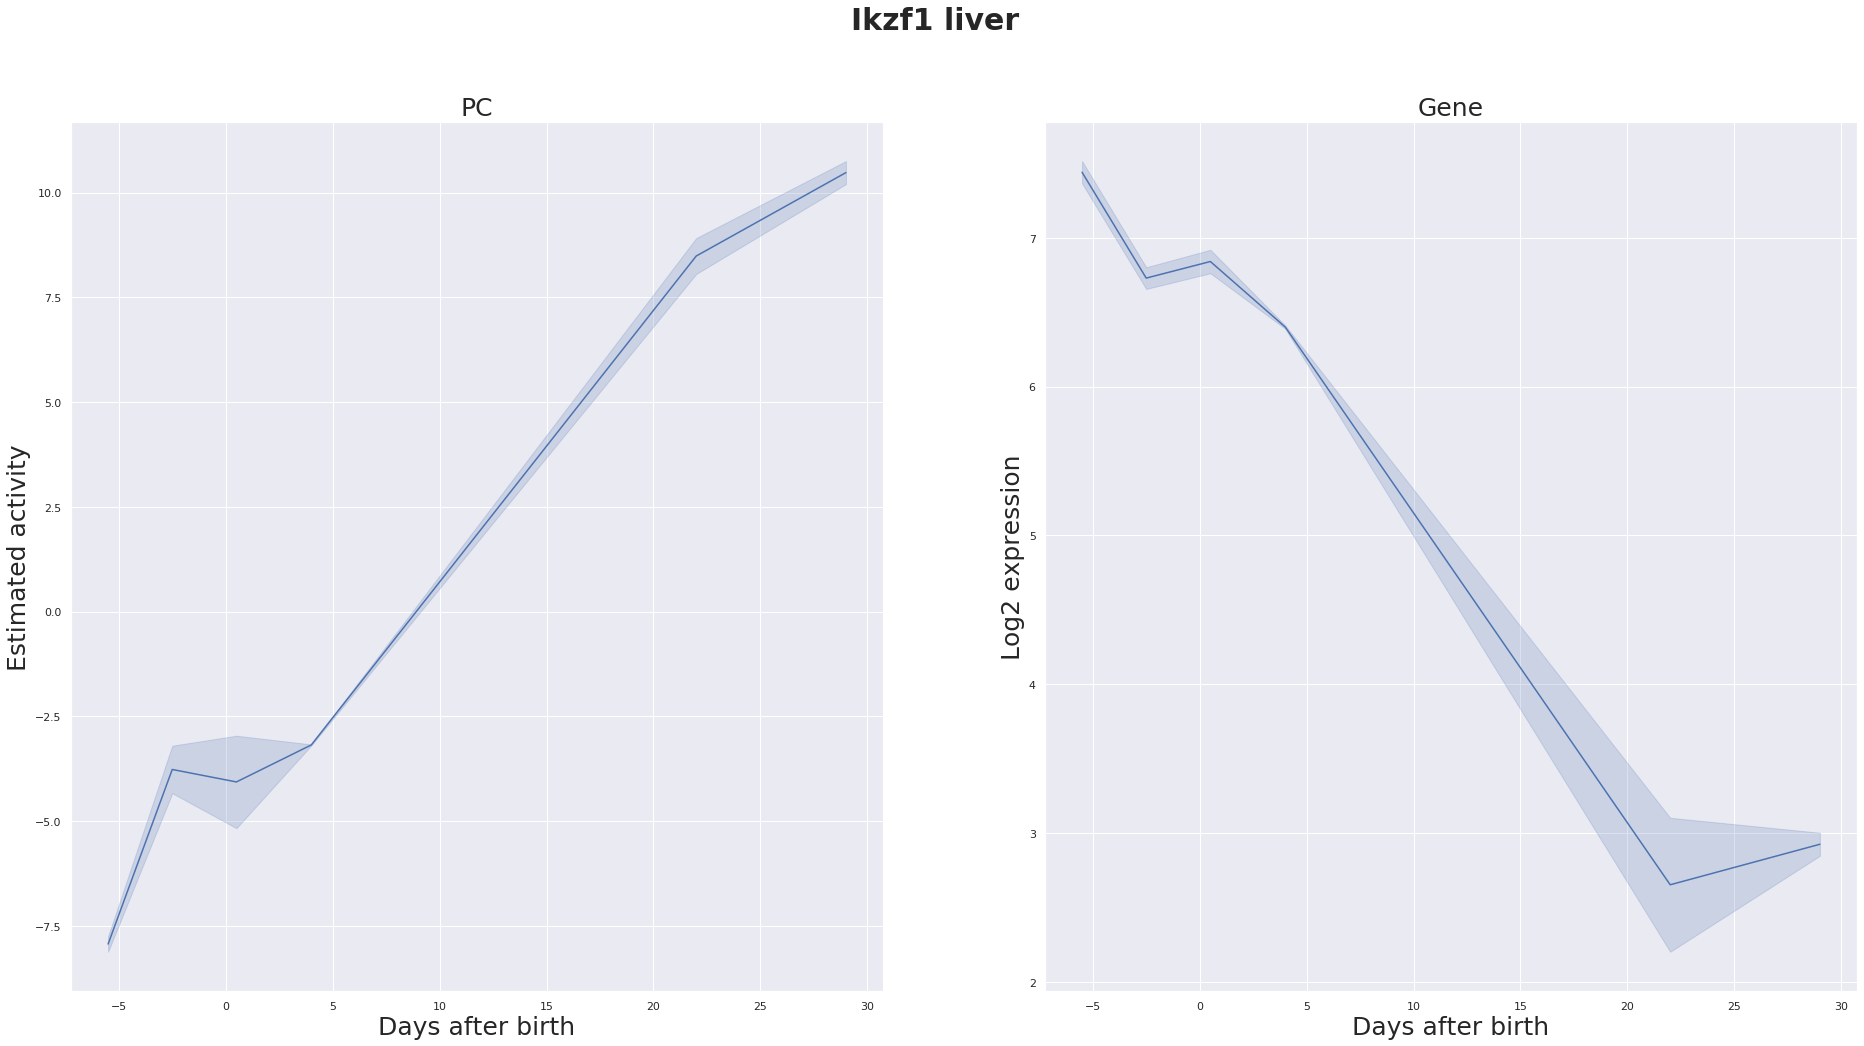
\includegraphics[width=6cm,height=3cm]{Figures&amp;Cover/Activity_Ikzf1_liver_NonePCremoved_filtering_False.png}
    \vspace{0.25cm}
    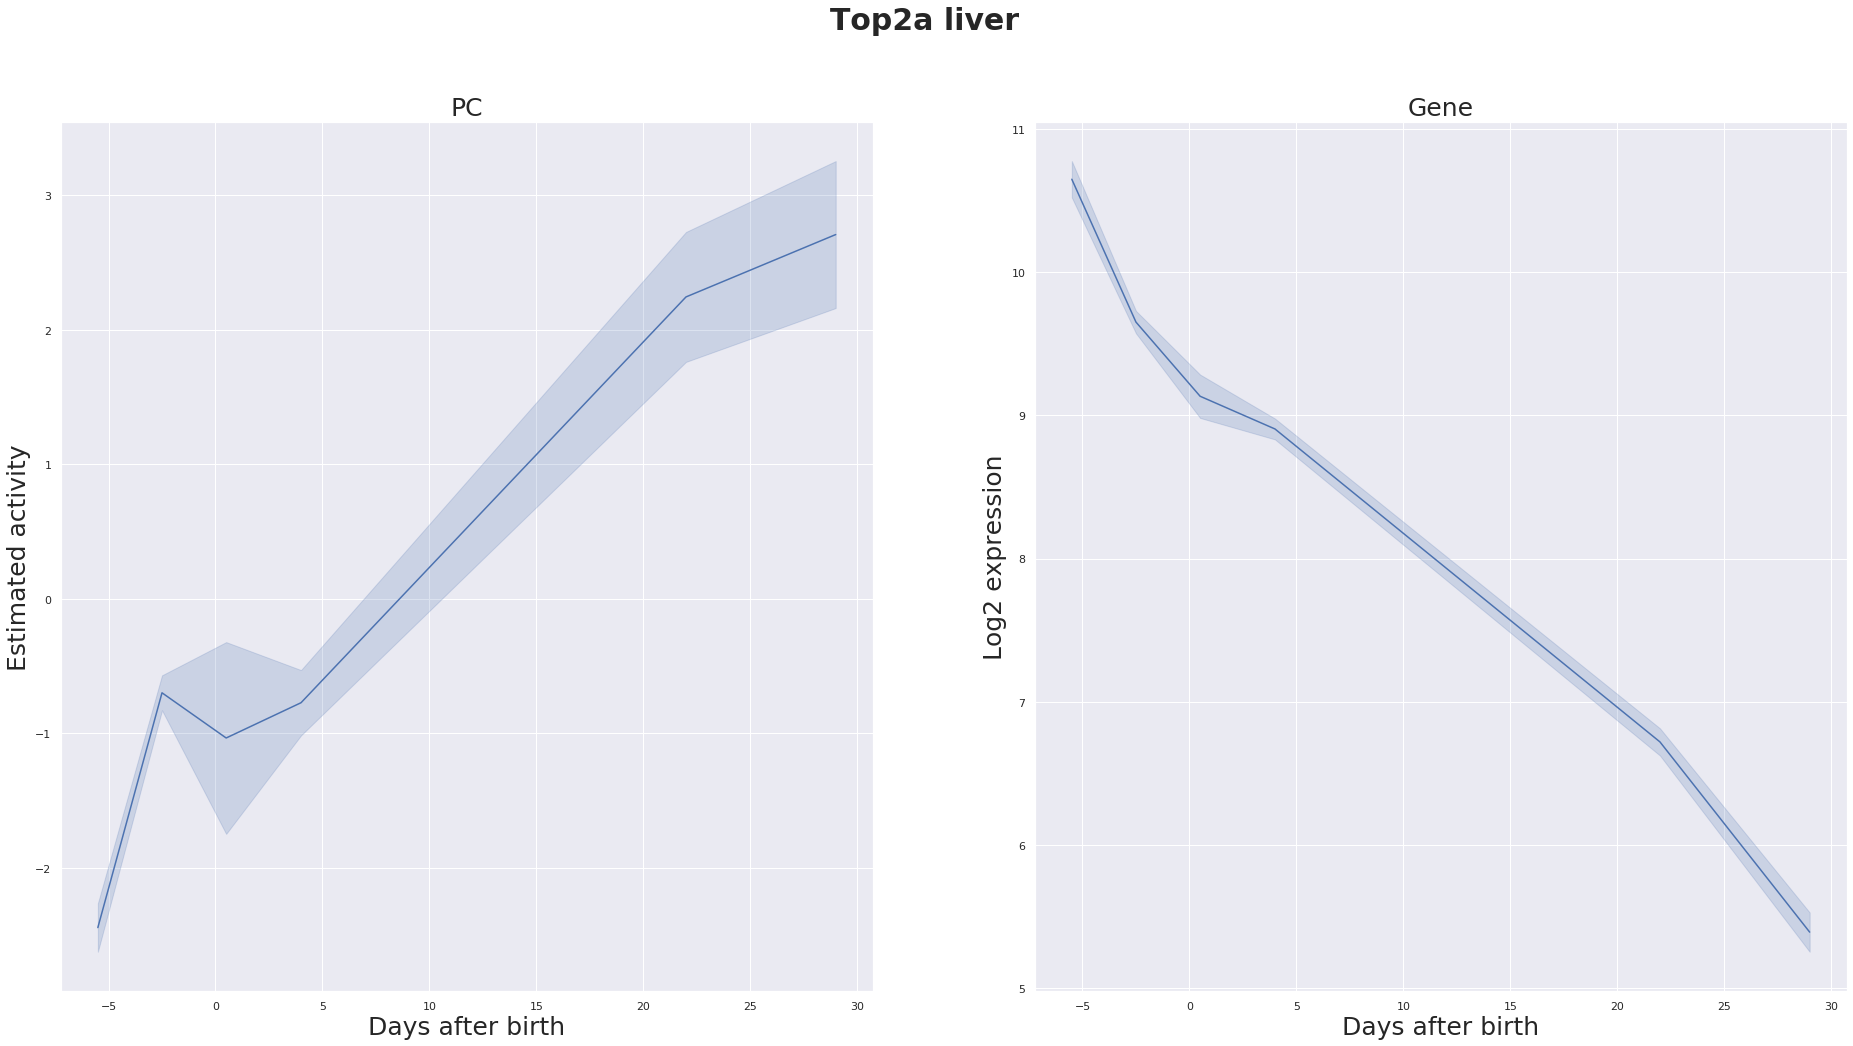
\includegraphics[width=6cm,height=3cm]{Figures&amp;Cover/Activity_Top2a_liver_NonePCremoved_filtering_False.png}
    \hspace{0.25cm}
    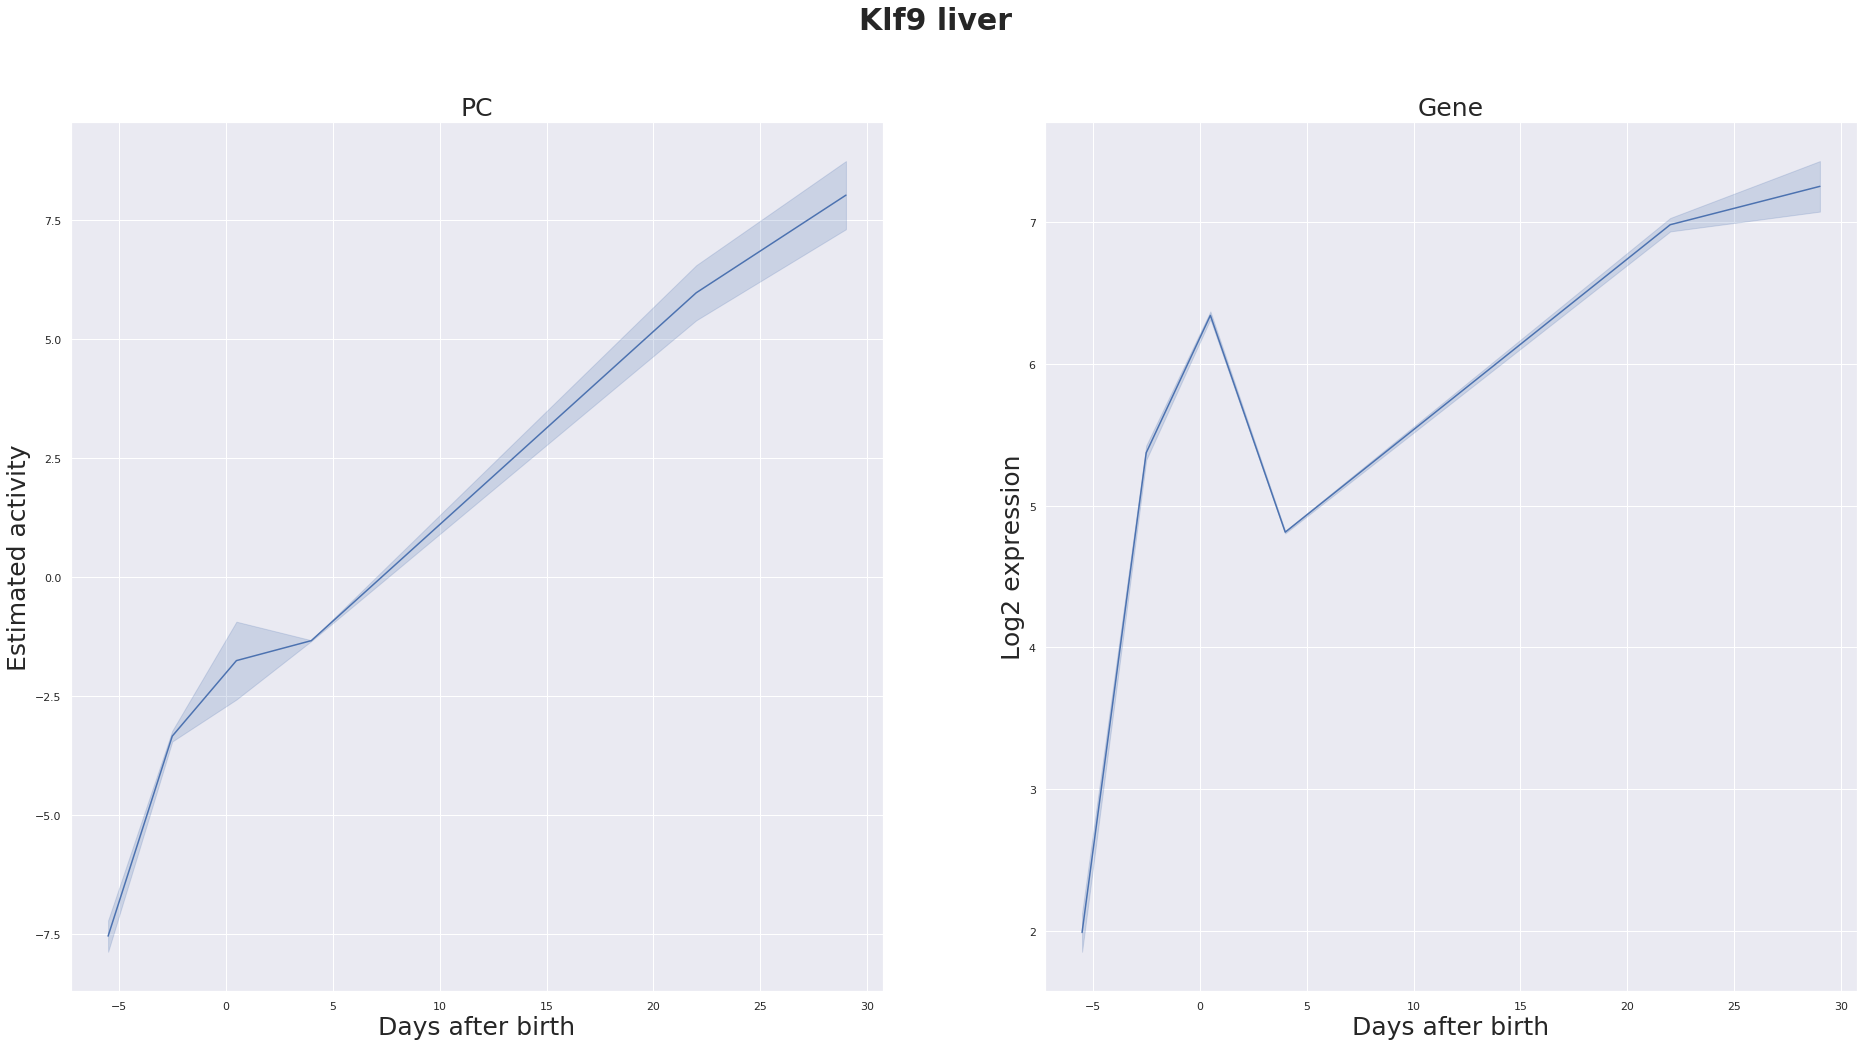
\includegraphics[width=6cm,height=3cm]{Figures&amp;Cover/Activity_Klf9_liver_NonePCremoved_filtering_False.png}
    \vspace{0.25cm}
    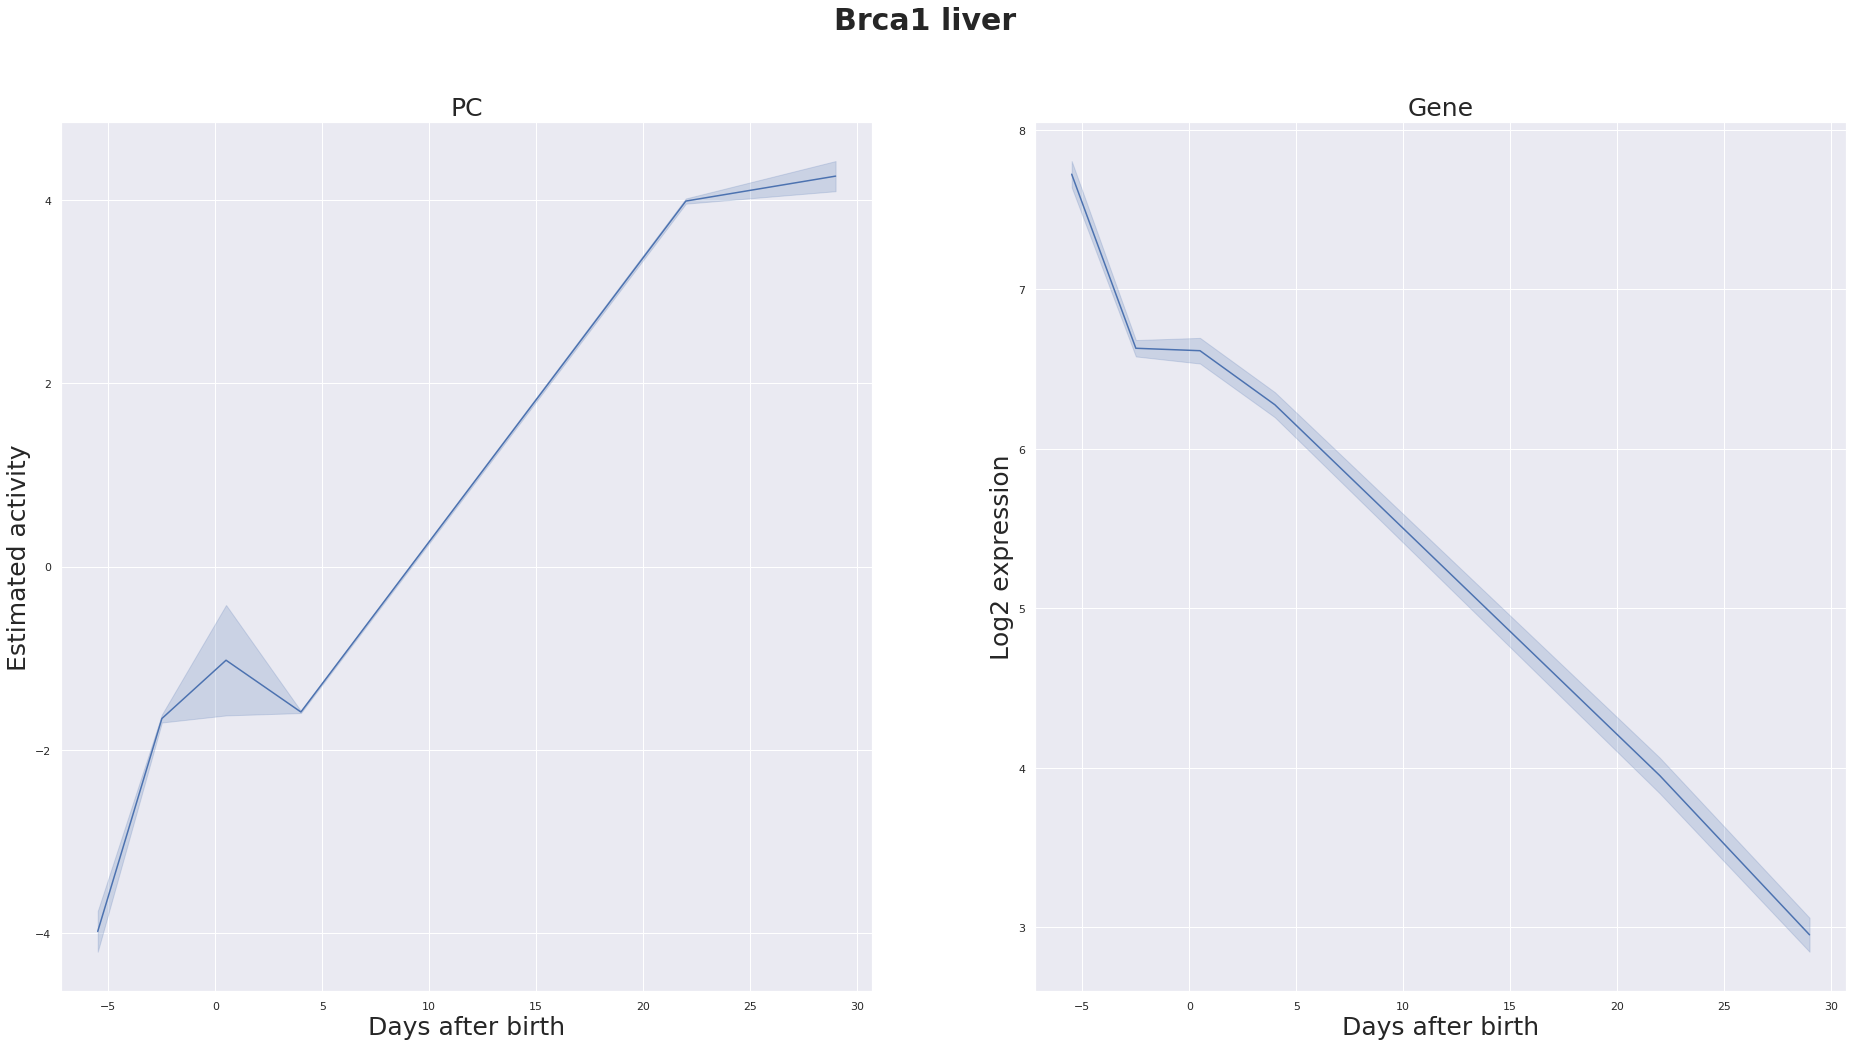
\includegraphics[width=6cm,height=3cm]{Figures&amp;Cover/Activity_Brca1_liver_NonePCremoved_filtering_False.png}
    \hspace{0.25cm}
    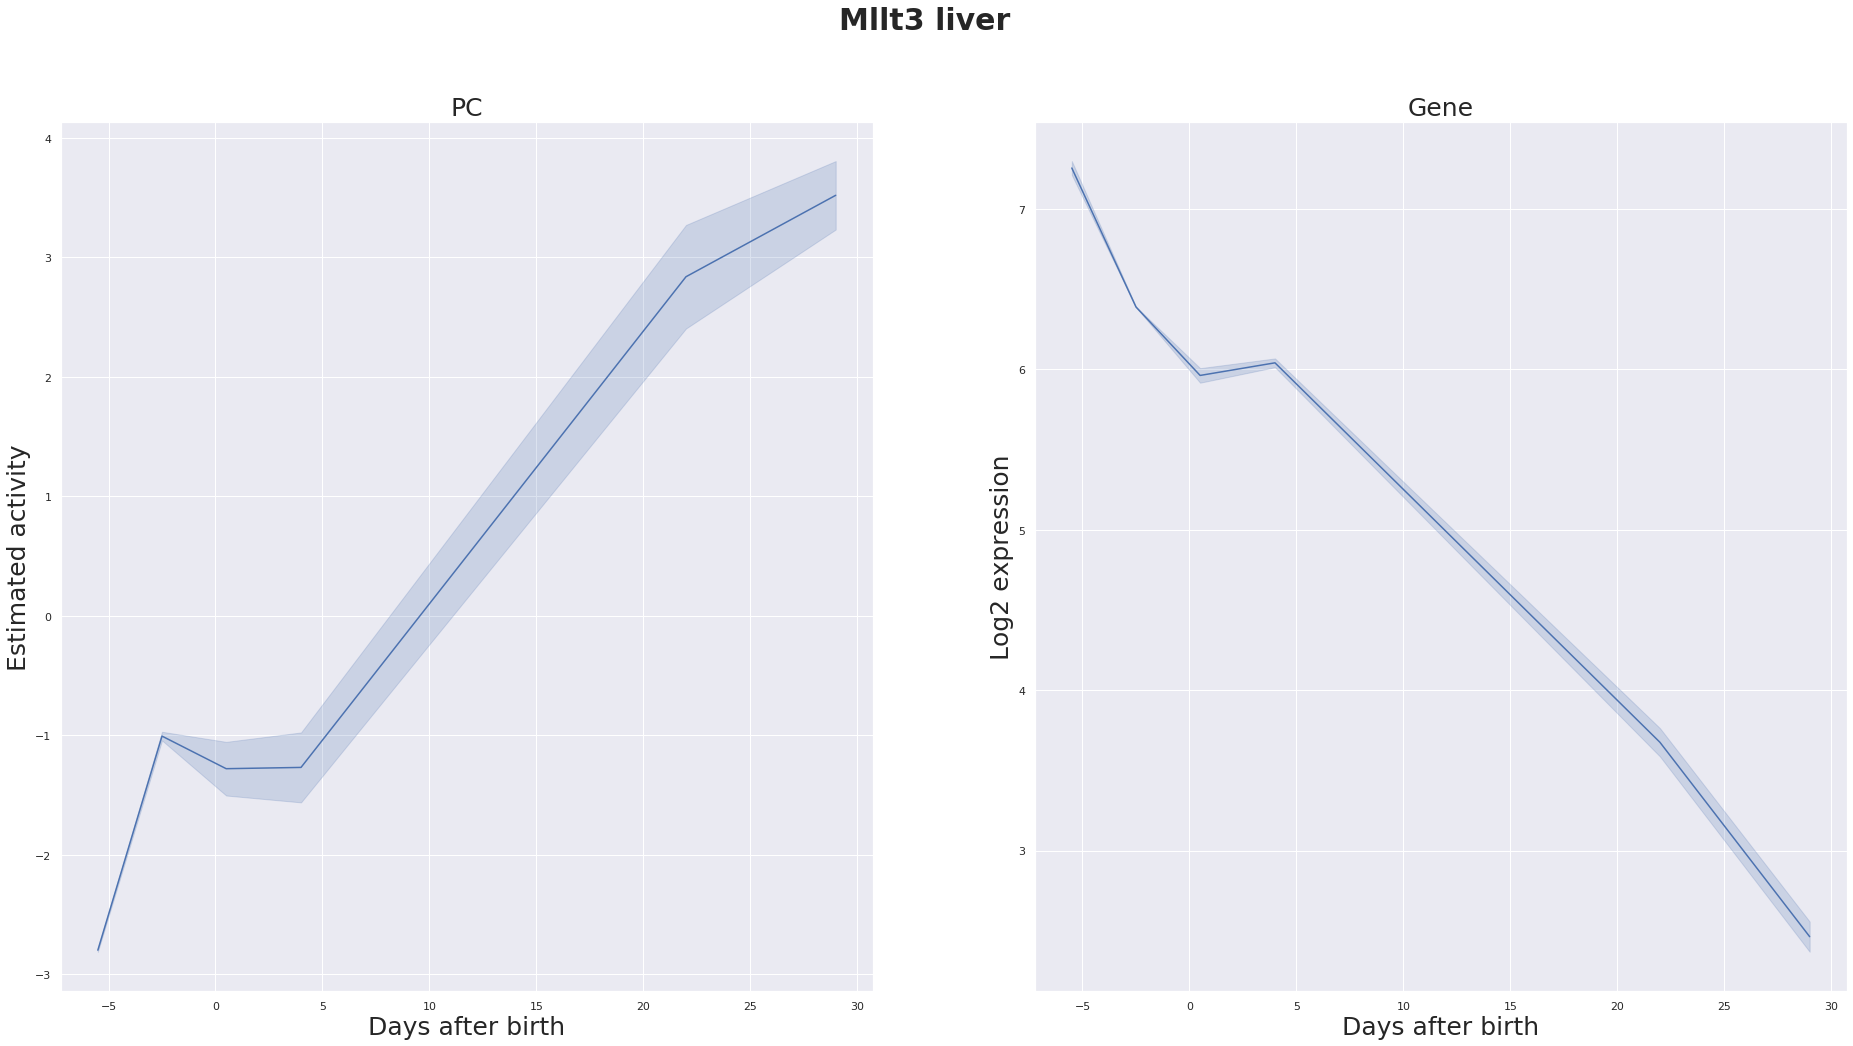
\includegraphics[width=6cm,height=3cm]{Figures&amp;Cover/Activity_Mllt3_liver_NonePCremoved_filtering_False.png}
    \vspace{0.25cm}
    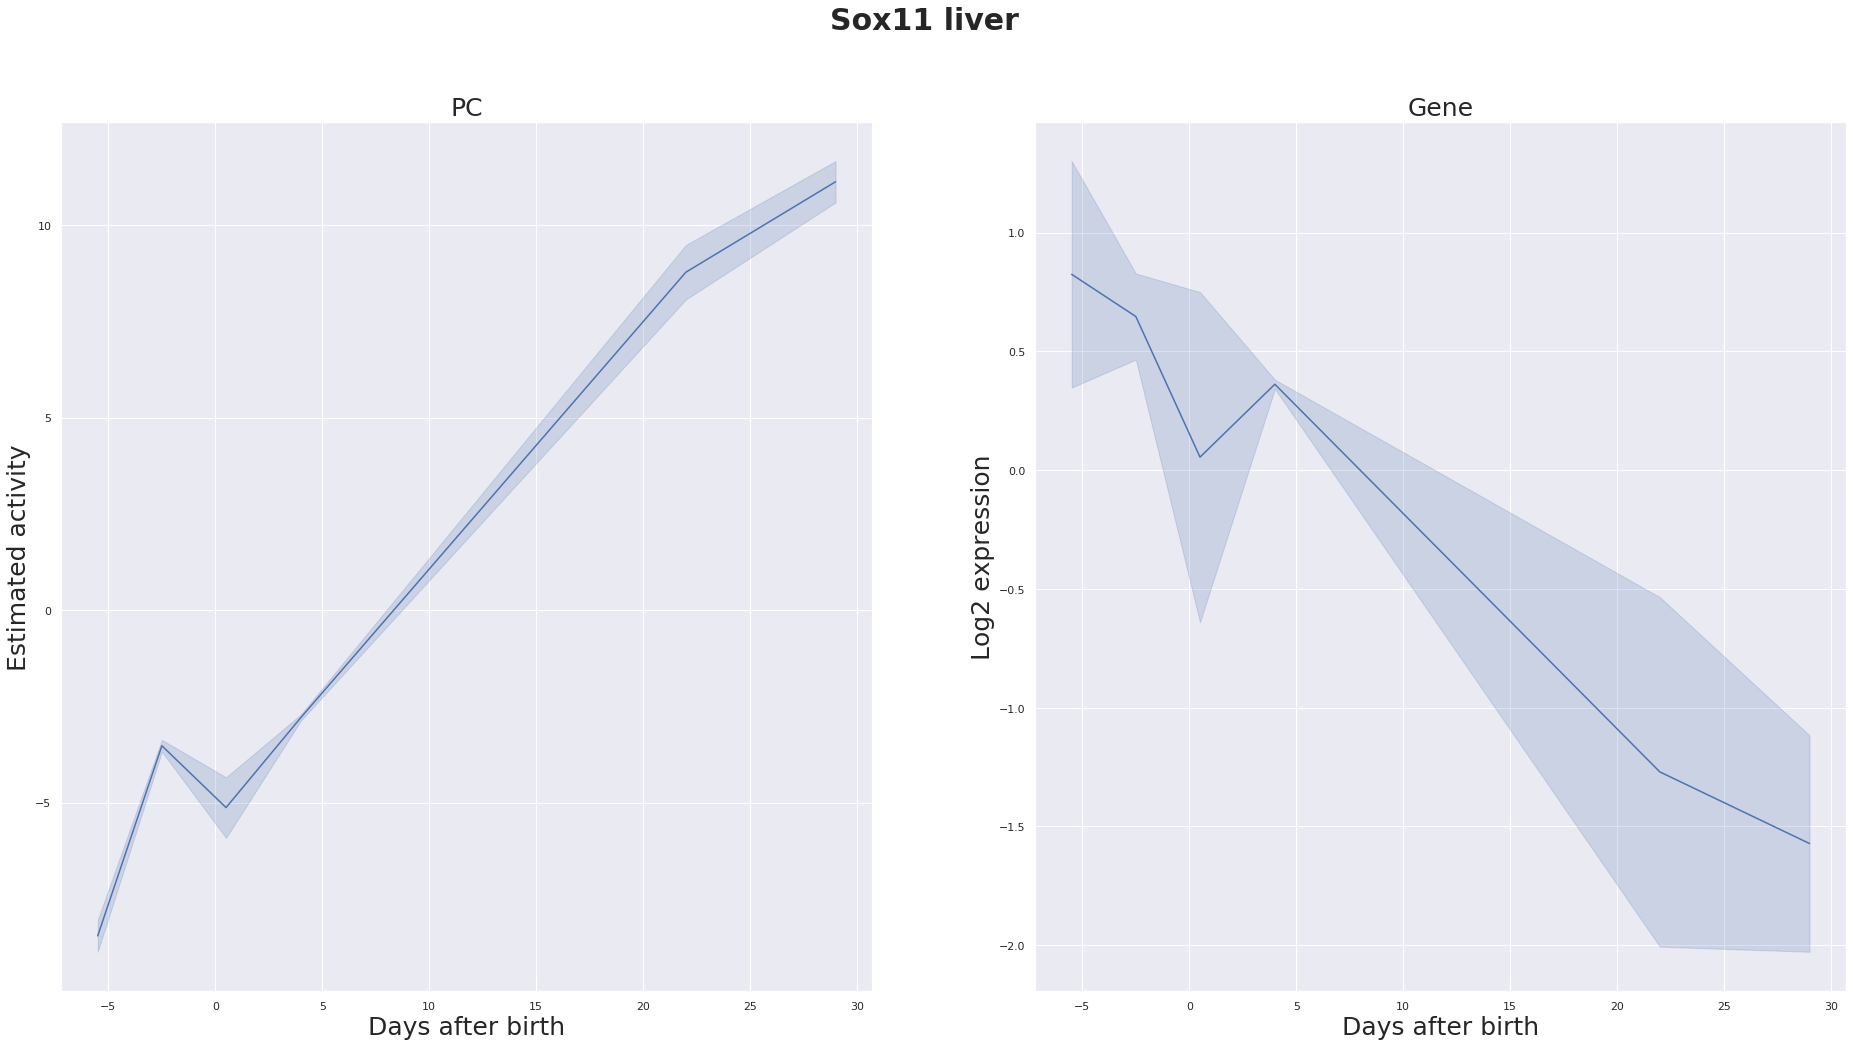
\includegraphics[width=6cm,height=3cm]{Figures&amp;Cover/Activity_Sox11_liver_NonePCremoved_filtering_False.png}
    \caption{\textbf{Estimated activities of Tal1, Lmo2, Ncapg, Ikzf1, Top2a, Klf9, Brca1, Mllt3 and Sox11 in mouse liver as a functions of the mices' age.} The activities were estimated by the first \ac{PC} of the mRNA expression data of the genes each \ac{TF} is likely to regulate (left figure of each pair) as well as directly through the transcription of the genes coding for each \ac{TF}, as log2-transformed \ac{RPM} transcript counts (right figure of each pair).}
    \label{fig:LiverEsts1}
\end{figure}

\begin{figure}
    \centering
    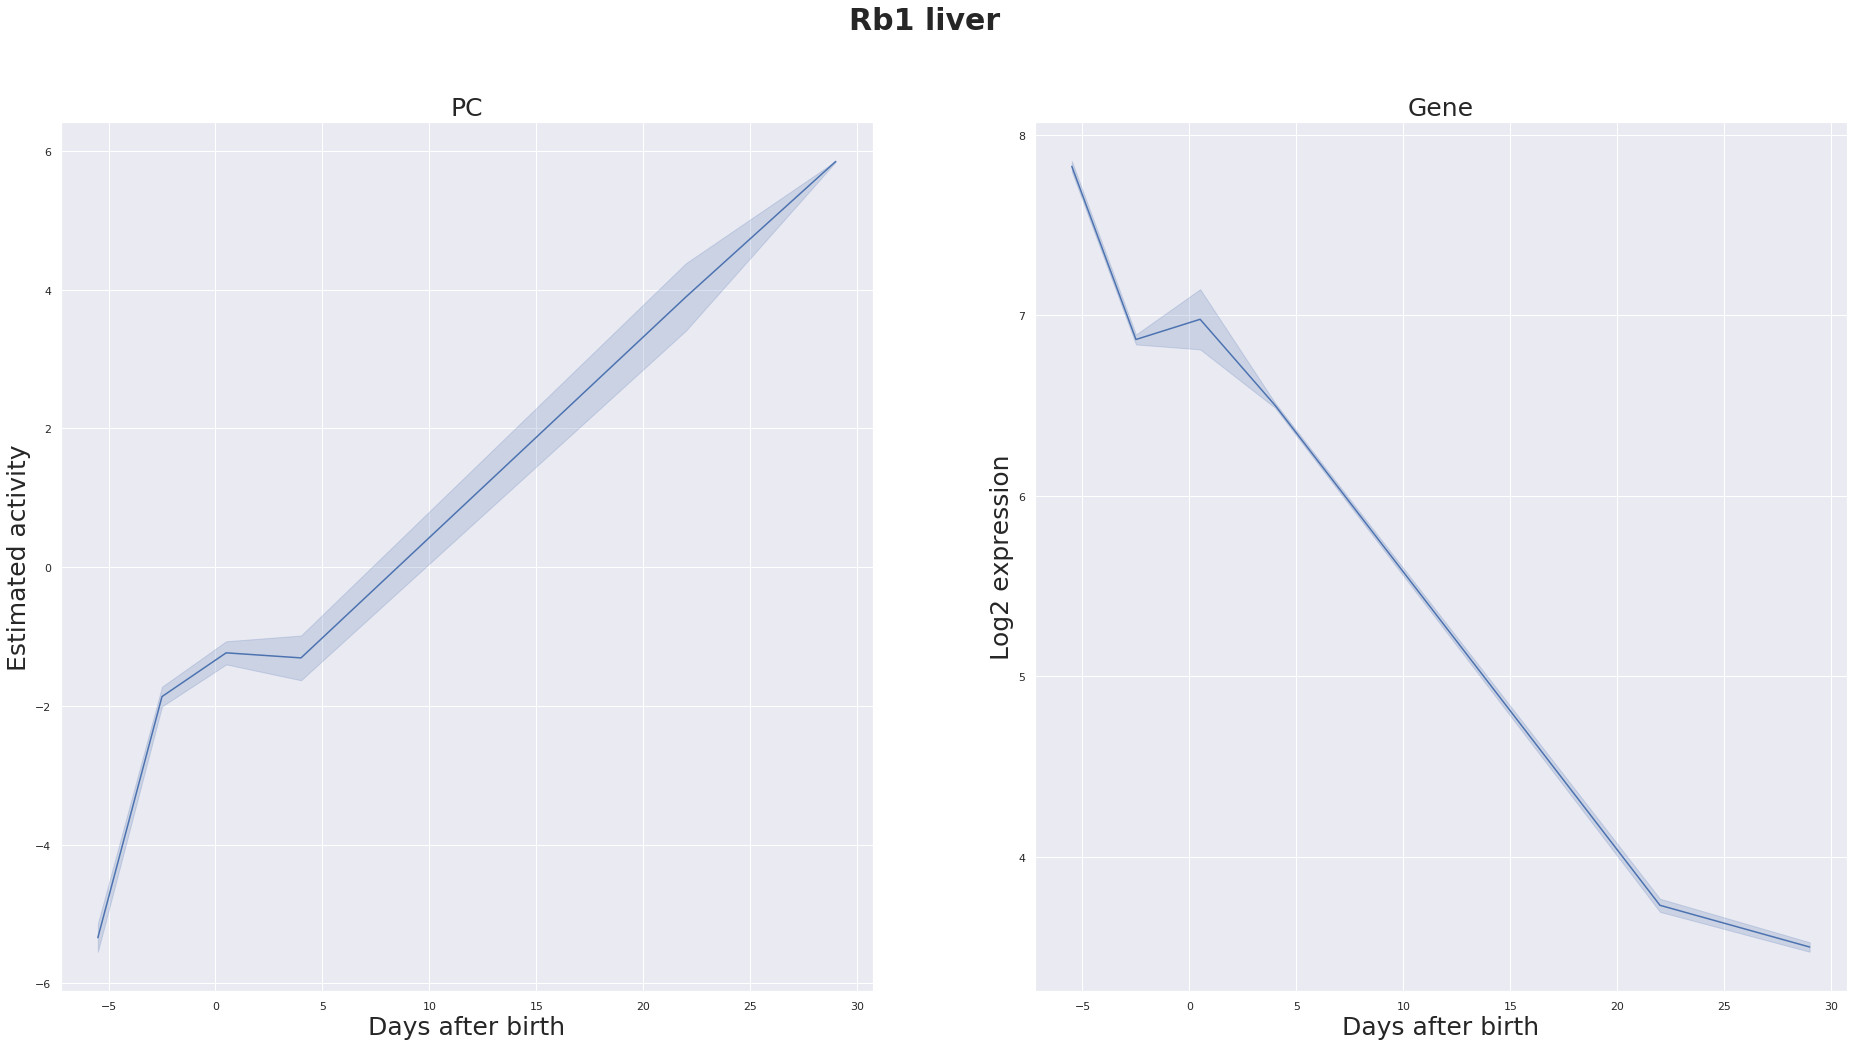
\includegraphics[width=6cm,height=3cm]{Figures&amp;Cover/Activity_Rb1_liver_NonePCremoved_filtering_False.png}
    \hspace{0.25cm}
    \vspace{0.25cm}
    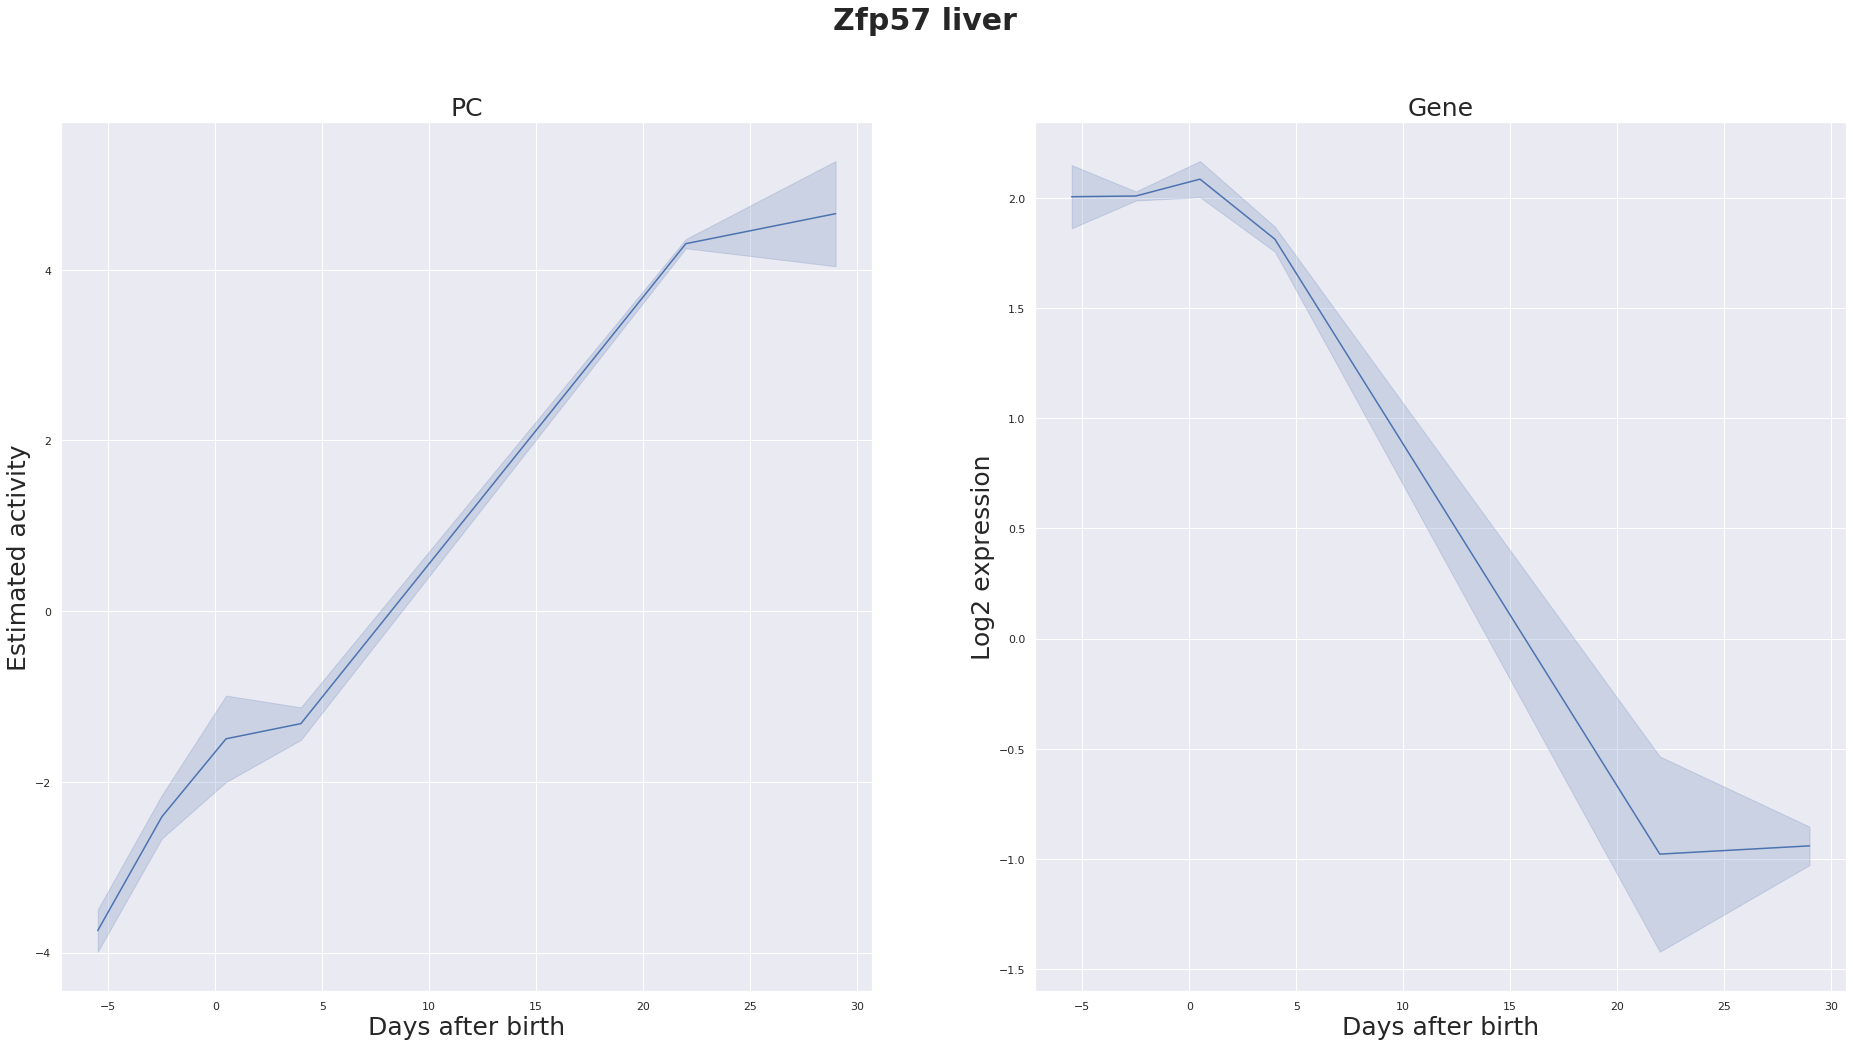
\includegraphics[width=6cm,height=3cm]{Figures&amp;Cover/Activity_Zfp57_liver_NonePCremoved_filtering_False.png}
    \vspace{0.25cm}
    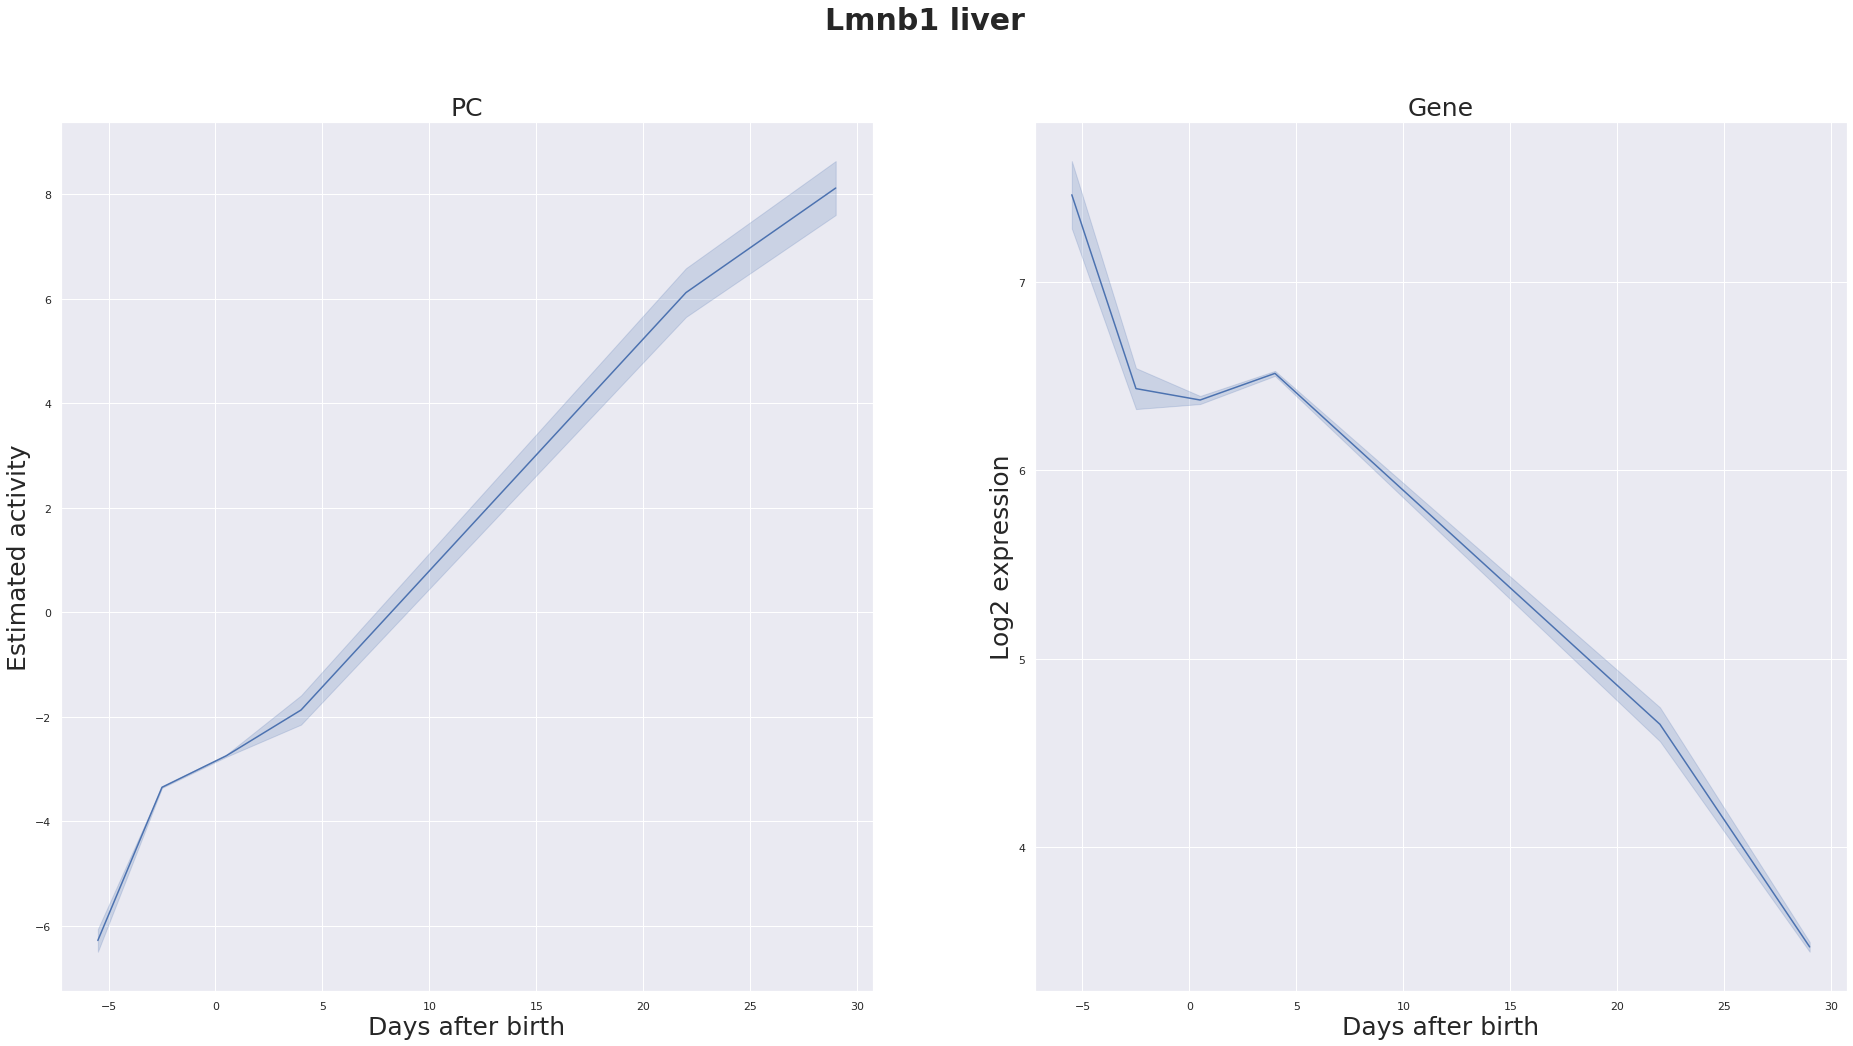
\includegraphics[width=6cm,height=3cm]{Figures&amp;Cover/Activity_Lmnb1_liver_NonePCremoved_filtering_False.png}
    \hspace{0.25cm}
    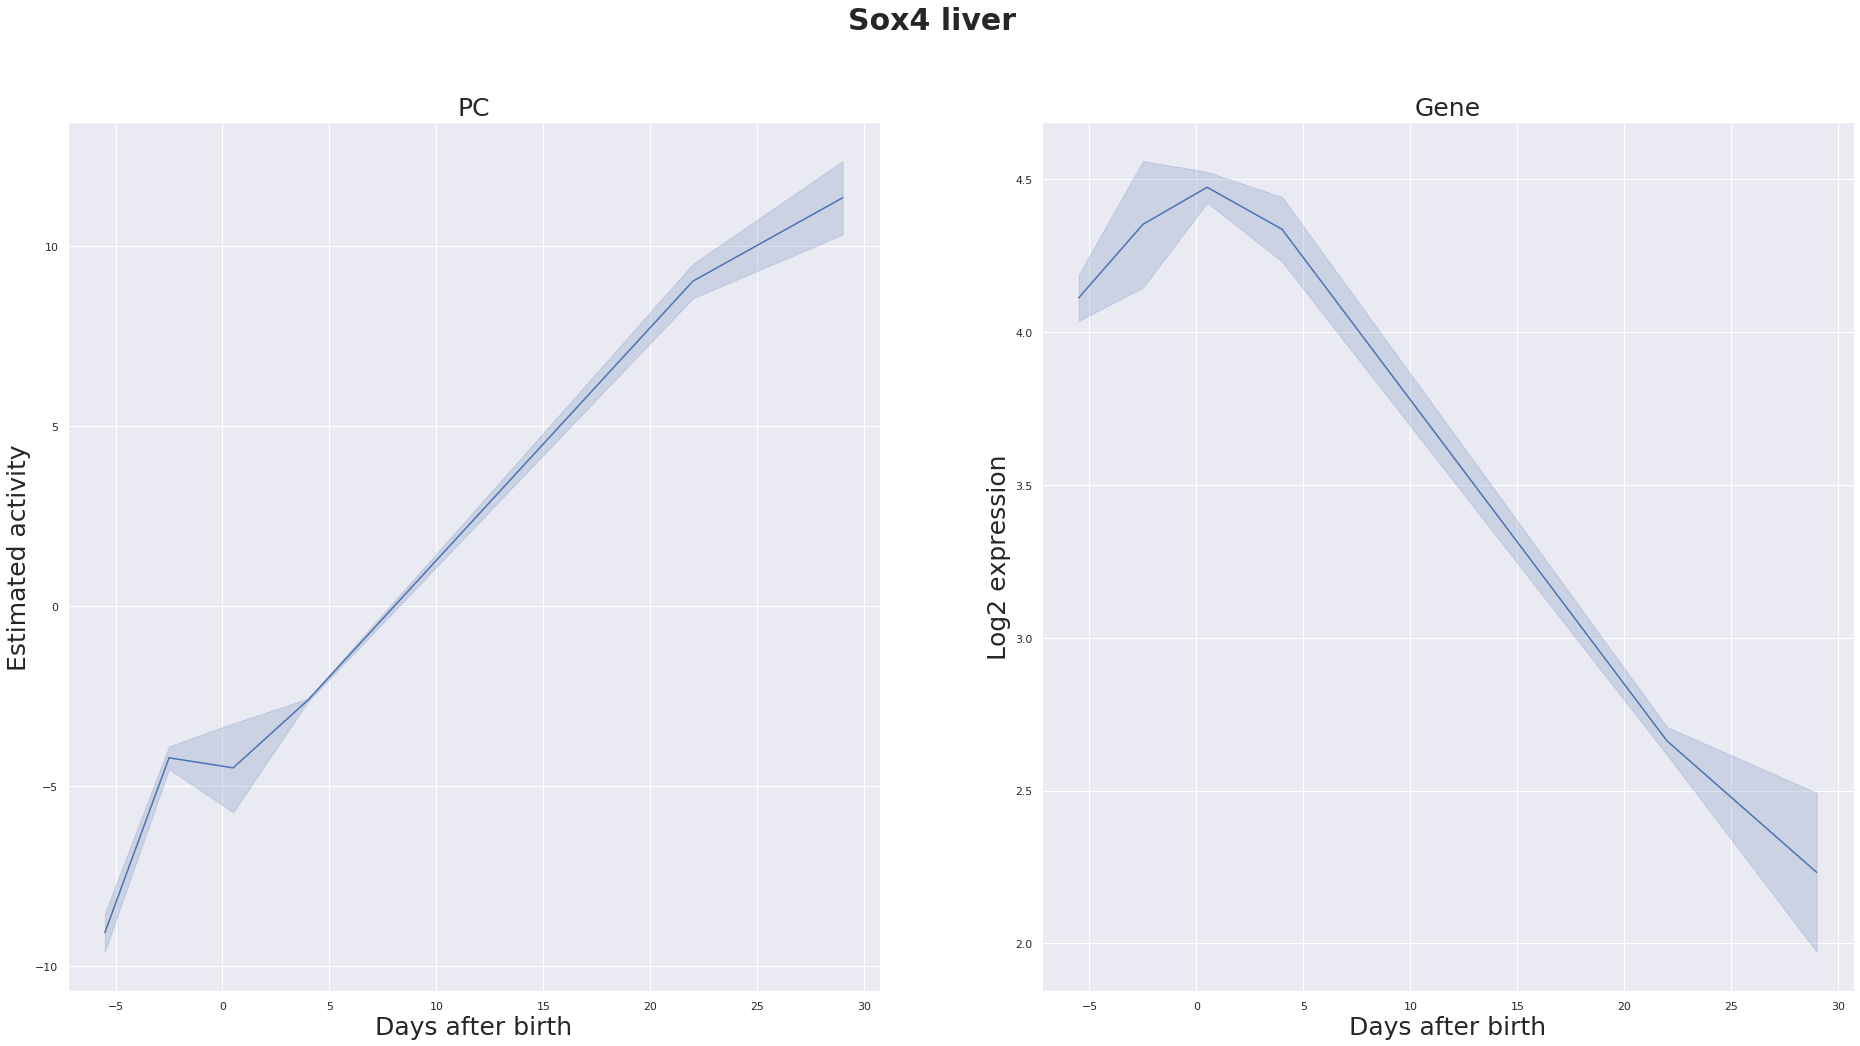
\includegraphics[width=6cm,height=3cm]{Figures&amp;Cover/Activity_Sox4_liver_NonePCremoved_filtering_False.png}
    \vspace{0.25cm}
    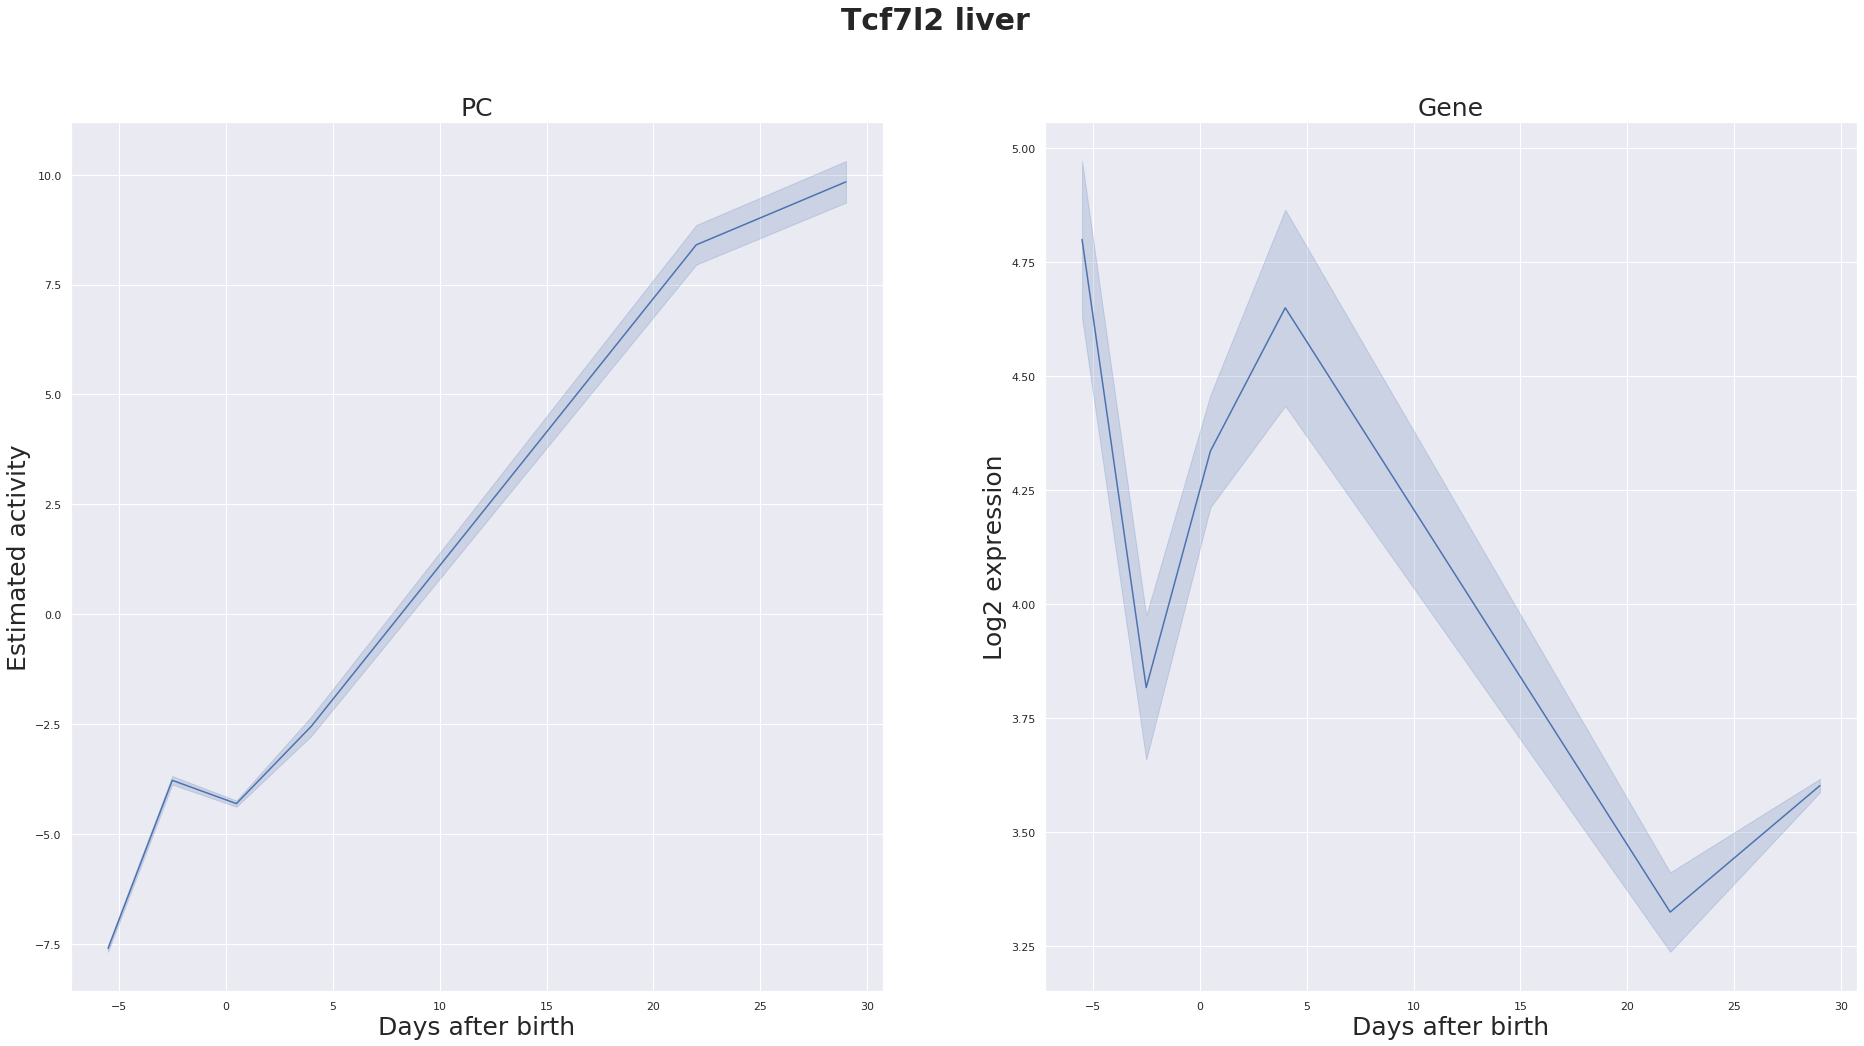
\includegraphics[width=6cm,height=3cm]{Figures&amp;Cover/Activity_Tcf7l2_liver_NonePCremoved_filtering_False.png}
    \hspace{0.25cm}
    \includegraphics[width=6cm,height=3cm]{Figures&amp;Cover/Activity_Nr1d2_liver_NonePCremoved_filtering_False.png}
    \vspace{0.25cm}
    \includegraphics[width=6cm,height=3cm]{Figures&amp;Cover/Activity_Nr3c1_liver_NonePCremoved_filtering_False.png}
    \hspace{0.25cm}
    \includegraphics[width=6cm,height=3cm]{Figures&amp;Cover/Activity_Satb2_liver_NonePCremoved_filtering_False.png}
    \caption{\textbf{Estimated activities of Rb1, Zfp57, Lmnb1, Sox4, Tc7l2, Nr1d2, Nr3c1 and Satb2 in mouse liver as a functions of the mices' age.} The activities were estimated by the first \ac{PC} of the mRNA expression data of the genes each \ac{TF} is likely to regulate (left figure of each pair) as well as directly through the transcription of the genes coding for each \ac{TF}, as log2-transformed \ac{RPM} transcript counts (right figure of each pair).}
    \label{fig:LiverEsts2}
\end{figure}

% PC REMOVED

\begin{figure}
    \centering
    \includegraphics[width=6cm,height=3cm]{Figures&amp;Cover/Activity_Tal1_brain_1PCremoved_filtering_False.png}
    \hspace{0.25cm}
    \vspace{0.25cm}
    \includegraphics[width=6cm,height=3cm]{Figures&amp;Cover/Activity_Lmo2_brain_1PCremoved_filtering_False.png}
    \vspace{0.25cm}
    \includegraphics[width=6cm,height=3cm]{Figures&amp;Cover/Activity_Ncapg_brain_1PCremoved_filtering_False.png}
    \hspace{0.25cm}
    \includegraphics[width=6cm,height=3cm]{Figures&amp;Cover/Activity_Ikzf1_brain_1PCremoved_filtering_False.png}
    \vspace{0.25cm}
    \includegraphics[width=6cm,height=3cm]{Figures&amp;Cover/Activity_Top2a_brain_1PCremoved_filtering_False.png}
    \hspace{0.25cm}
    \includegraphics[width=6cm,height=3cm]{Figures&amp;Cover/Activity_Klf9_brain_1PCremoved_filtering_False.png}
    \vspace{0.25cm}
    \includegraphics[width=6cm,height=3cm]{Figures&amp;Cover/Activity_Brca1_brain_1PCremoved_filtering_False.png}
    \hspace{0.25cm}
    \includegraphics[width=6cm,height=3cm]{Figures&amp;Cover/Activity_Mllt3_brain_1PCremoved_filtering_False.png}
    \vspace{0.25cm}
    \includegraphics[width=6cm,height=3cm]{Figures&amp;Cover/Activity_Sox11_brain_1PCremoved_filtering_False.png}
    \caption{\textbf{Estimated activities of Tal1, Lmo2, Ncapg, Ikzf1, Top2a, Klf9, Brca1, Mllt3 and Sox11 in mouse brains as a functions of the mices' age, calculated using mRNA expression data from which the first \ac{PC} had been removed.} The activities were estimated by the first \ac{PC} of the mRNA expression data of the genes each \ac{TF} is likely to regulate (left figure of each pair) as well as directly through the transcription of the genes coding for each \ac{TF}, as log2-transformed \ac{RPM} transcript counts (right figure of each pair).}
    \label{fig:BrainEstsClean1}
\end{figure}    
    
\begin{figure}
    \centering
    \includegraphics[width=6cm,height=3cm]{Figures&amp;Cover/Activity_Rb1_brain_1PCremoved_filtering_False.png}
    \hspace{0.25cm}
    \vspace{0.25cm}
    \includegraphics[width=6cm,height=3cm]{Figures&amp;Cover/Activity_Zfp57_brain_1PCremoved_filtering_False.png}
    \vspace{0.25cm}
    \includegraphics[width=6cm,height=3cm]{Figures&amp;Cover/Activity_Lmnb1_brain_1PCremoved_filtering_False.png}
    \hspace{0.25cm}
    \includegraphics[width=6cm,height=3cm]{Figures&amp;Cover/Activity_Sox4_brain_1PCremoved_filtering_False.png}
    \vspace{0.25cm}
    \includegraphics[width=6cm,height=3cm]{Figures&amp;Cover/Activity_Tcf7l2_brain_1PCremoved_filtering_False.png}
    \hspace{0.25cm}
    \includegraphics[width=6cm,height=3cm]{Figures&amp;Cover/Activity_Nr1d2_brain_1PCremoved_filtering_False.png}
    \vspace{0.25cm}
    \includegraphics[width=6cm,height=3cm]{Figures&amp;Cover/Activity_Nr3c1_brain_1PCremoved_filtering_False.png}
    \hspace{0.25cm}
    \includegraphics[width=6cm,height=3cm]{Figures&amp;Cover/Activity_Satb2_brain_1PCremoved_filtering_False.png}
    \caption{\textbf{Estimated activities of Rb1, Zfp57, Lmnb1, Sox4, Tc7l2, Nr1d2, Nr3c1 and Satb2 in mouse brains as a functions of the mices' age, calculated using mRNA expression data from which the first \ac{PC} had been removed.} The activities were estimated by the first \ac{PC} of the mRNA expression data of the genes each \ac{TF} is likely to regulate (left figure of each pair) as well as directly through the transcription of the genes coding for each \ac{TF}, as log2-transformed \ac{RPM} transcript counts (right figure of each pair).}
    \label{fig:BrainEstsClean2}
\end{figure}

\begin{figure}
    \centering
    \includegraphics[width=6cm,height=3cm]{Figures&amp;Cover/Activity_Tal1_liver_1PCremoved_filtering_False.png}
    \hspace{0.25cm}
    \vspace{0.25cm}
    \includegraphics[width=6cm,height=3cm]{Figures&amp;Cover/Activity_Lmo2_liver_1PCremoved_filtering_False.png}
    \vspace{0.25cm}
    \includegraphics[width=6cm,height=3cm]{Figures&amp;Cover/Activity_Ncapg_liver_1PCremoved_filtering_False.png}
    \hspace{0.25cm}
    \includegraphics[width=6cm,height=3cm]{Figures&amp;Cover/Activity_Ikzf1_liver_1PCremoved_filtering_False.png}
    \vspace{0.25cm}
    \includegraphics[width=6cm,height=3cm]{Figures&amp;Cover/Activity_Top2a_liver_1PCremoved_filtering_False.png}
    \hspace{0.25cm}
    \includegraphics[width=6cm,height=3cm]{Figures&amp;Cover/Activity_Klf9_liver_1PCremoved_filtering_False.png}
    \vspace{0.25cm}
    \includegraphics[width=6cm,height=3cm]{Figures&amp;Cover/Activity_Brca1_liver_1PCremoved_filtering_False.png}
    \hspace{0.25cm}
    \includegraphics[width=6cm,height=3cm]{Figures&amp;Cover/Activity_Mllt3_liver_1PCremoved_filtering_False.png}
    \vspace{0.25cm}
    \includegraphics[width=6cm,height=3cm]{Figures&amp;Cover/Activity_Sox11_liver_1PCremoved_filtering_False.png}
    \caption{\textbf{Estimated activities of Tal1, Lmo2, Ncapg, Ikzf1, Top2a, Klf9, Brca1, Mllt3 and Sox11 in mouse liver as a functions of the mices' age, calculated using mRNA expression data from which the first \ac{PC} had been removed.} The activities were estimated by the first \ac{PC} of the mRNA expression data of the genes each \ac{TF} is likely to regulate (left figure of each pair) as well as directly through the transcription of the genes coding for each \ac{TF}, as log2-transformed \ac{RPM} transcript counts (right figure of each pair).}
    \label{fig:LiverEstsClean1}
\end{figure}

\begin{figure}
    \centering
    \includegraphics[width=6cm,height=3cm]{Figures&amp;Cover/Activity_Rb1_liver_1PCremoved_filtering_False.png}
    \hspace{0.25cm}
    \vspace{0.25cm}
    \includegraphics[width=6cm,height=3cm]{Figures&amp;Cover/Activity_Zfp57_liver_1PCremoved_filtering_False.png}
    \vspace{0.25cm}
    \includegraphics[width=6cm,height=3cm]{Figures&amp;Cover/Activity_Lmnb1_liver_1PCremoved_filtering_False.png}
    \hspace{0.25cm}
    \includegraphics[width=6cm,height=3cm]{Figures&amp;Cover/Activity_Sox4_liver_1PCremoved_filtering_False.png}
    \vspace{0.25cm}
    \includegraphics[width=6cm,height=3cm]{Figures&amp;Cover/Activity_Tcf7l2_liver_1PCremoved_filtering_False.png}
    \hspace{0.25cm}
    \includegraphics[width=6cm,height=3cm]{Figures&amp;Cover/Activity_Nr1d2_liver_1PCremoved_filtering_False.png}
    \vspace{0.25cm}
    \includegraphics[width=6cm,height=3cm]{Figures&amp;Cover/Activity_Nr3c1_liver_1PCremoved_filtering_False.png}
    \hspace{0.25cm}
    \includegraphics[width=6cm,height=3cm]{Figures&amp;Cover/Activity_Satb2_liver_1PCremoved_filtering_False.png}
    \caption{\textbf{Estimated activities of Rb1, Zfp57, Lmnb1, Sox4, Tc7l2, Nr1d2, Nr3c1 and Satb2 in mouse liver as a functions of the mices' age, calculated using mRNA expression data from which the first \ac{PC} had been removed.} The activities were estimated by the first \ac{PC} of the mRNA expression data of the genes each \ac{TF} is likely to regulate (left figure of each pair) as well as directly through the transcription of the genes coding for each \ac{TF}, as log2-transformed \ac{RPM} transcript counts (right figure of each pair).}
    \label{fig:LiverEstsClean2}
\end{figure}

% Tailmatter inserts the back cover page (if enabled)
\tailmatter

\end{document}
